% LaTeX source for book ``代数学方法'' in Chinese
% Copyright 2024  李文威 (Wen-Wei Li).
% Permission is granted to copy, distribute and/or modify this
% document under the terms of the Creative Commons
% Attribution 4.0 International (CC BY 4.0)
% http://creativecommons.org/licenses/by/4.0/

% To be included
\chapter{范畴论拾遗}\label{sec:categories}
顾名思义, 本章介绍后续各章所需的若干范畴论工具, 方便读者温故知新. 部分内容见于 \cite{Li1} 或类似教材, 然而出于回顾概念和统一符号的理由, 本章依然予以重述. 其他基本术语则可参照本书导言.

\begin{itemize}
	\item 在 \S\S\ref{sec:subquot}---\ref{sec:images}, 我们先简单介绍子对象和商对象, 当然也包括单态射和满态射的一般性质, 然后介绍态射 $f$ 的像 $\Image(f)$ 和余像 $\Coim(f)$, 以及满足``像即余像''的态射, 称为严格态射. 这些是适用于一般范畴的基本概念.
	\item \S\S\ref{sec:Ker-Coker}---\ref{sec:linear-cat} 是本章的线性部分, 该处介绍了态射集上具有加法群结构的一类特殊范畴, 称为 $\cate{Ab}$-范畴; 保持态射加法的函子称为加性函子. 对这些范畴可以定义态射的核及余核, 作为模同态的核及余核的推广. 具备零对象和有限积的 $\cate{Ab}$-范畴称为加性范畴; 在加性范畴中可以讨论对象的有限直和, 而有限直和之间的态射能够以类似于矩阵运算的方式进行操作.
	
	推而广之, 加法结构还能升级为来自某个交换环 $\Bbbk$ 的纯量乘法, 由此得到 $\Bbbk\dcate{Mod}$-范畴和 $\Bbbk$-线性范畴的概念. 这些带有线性结构的范畴是本书的主要关切.
	
	\item \S\S\ref{sec:limit-functor}---\ref{sec:filtered-indlim} 是关于极限的基础知识. 特别地, 定义 \ref{def:create-limit} 将引入关于一个函子 $F: \mathcal{C} \to \mathcal{D}$ 是否保 (自 $\mathcal{C}$ 到 $\mathcal{D}$) 或生 (自 $\mathcal{D}$ 到 $\mathcal{C}$) 极限的说法, 此外我们也探讨共尾函子和滤过归纳极限, 这些术语方便而且重要.
	
	\item \S\S\ref{sec:Kan-extension}---\ref{sec:Kan-as-limit} 讨论的左和右 Kan 延拓是范畴论的一类基本操作. 适当条件下, 它们可以用 $\varinjlim$ 或 $\varprojlim$ 来构造; 论证不无曲折, 但思路是简单的, 要点在于以极限来表述函子延拓问题的``最佳逼近''. 我们也记录一则并不显然的定理 \ref{prop:Quillen-adjunction-gen}, 它阐明绝对左/右 Kan 延拓和伴随对之间的联系.

	\item \S\ref{sec:cat-localization} 介绍的 Gabriel--Zisman 局部化 (本书简称``局部化'') 是向范畴中的一族态射 $S$ 形式地添逆的构造, 它可类比于环的局部化, 但具体细节复杂不少; 为了对取逆后的产物有更好的掌控, 实践中经常设 $S$ 为定义 \ref{def:multiplicative-family} 所谓的乘性系. 局部化在本书的主要应用是构造导出范畴, 其次则是用于在 \S\ref{sec:Serre-subcat} 定义 Abel 范畴的 Serre 商. \S\ref{sec:functor-localization} 将说明如何沿着范畴的局部化作 Kan 延拓, 不妨将之设想为函子的局部化, 这是之后理解导出函子的关键.
	
	\item \S\ref{sec:AFT} 讨论的伴随函子定理刻画了左伴随或右伴随函子在适当条件下的存在性; 在本书中, 它主要应用于 \S\ref{sec:Grothendieck-cat} 对 Grothendieck 范畴的研究. 伴随函子定理在数学中的用处不止于此, 所以本节有其独立价值, 而该处探讨的生成元和余生成元 (定义 \ref{def:generators}) 也是必须掌握的概念.
\end{itemize}

本章内容较多地借鉴了 \cite{KS06, Rie16}.

\begin{wenxintishi}
	Abel 范畴和复形的基本理论仅需要本章的 \S\S\ref{sec:subquot}---\ref{sec:linear-cat}, 其后的 \S\S\ref{sec:limit-functor}---\ref{sec:filtered-indlim} 对此起到辅助作用, 本书其他章节也会反复引用. 导出范畴理论涉及本章的 \S\S\ref{sec:Kan-extension}---\ref{sec:functor-localization}, 相关内容的用途不限于此, 但读者可衡量自身需求, 待学习导出范畴之前再行阅读. 最后的 \S\ref{sec:AFT} 仅应用于 \S\ref{sec:Grothendieck-cat}, 然而其中关于生成元和余生成元的知识是必备的, 读者必要时可回头查阅.
\end{wenxintishi}

\section{子商}\label{sec:subquot}
首先回顾单态射和满态射的概念. 选定范畴 $\mathcal{C}$.

\begin{itemize}
	\item 态射 $f: X \to Y$ 称为\emph{单态射}, 也标作 $f: X \hookrightarrow Y$, 如果左消去律成立:
	\[ \forall T \in \Obj(\mathcal{C}), \; \forall g,h: T \to X , \quad fg=fh \iff g=h; \]
	\item 态射 $f: X \to Y$ 称为\emph{满态射}, 也标作 $f: X \twoheadrightarrow Y$, 如果右消去律成立:
	\[ \forall T \in \Obj(\mathcal{C}), \; \forall g,h: Y \to T, \quad gf=hf \iff g=h. \]
\end{itemize}
\index{dantaishe@单态射 (monomorphism)}
\index{mantaishe@满态射 (epimorphism)}

不难读出 $f: X \to Y$ 单等价于 $f_*: \Hom(T, X) \to \Hom(T, Y)$ 对所有 $T$ 皆单; $f: X \to Y$ 满等价于 $f^*: \Hom(Y, T) \to \Hom(X, T)$ 对所有 $T$ 皆单. 态射的单性和满性相互对偶: $f$ 单当且仅当 $f^{\opp}$ 满.

\begin{example}
	若一对态射 $f, g: X \to Y$ 的等化子 $\Ker(f,g)$ 存在, 则泛性质说明典范态射 $\iota: \Ker(f,g) \to X$ 单. 同理, 若余等化子 $\Coker(f,g)$ 存在则典范态射 $p: Y \to \Coker(f,g)$ 满. 另一则平凡的观察则是: 若 $\mathcal{C}$ 有零对象, 依惯例记为 $0$, 则 $0 \to X$ 单而 $X \to 0$ 满. 请读者验证这些细节.
\end{example}

\begin{proposition}\label{prop:epi-mono-isomorphism}
	考虑态射 $X \xrightarrow{a} Y \xrightarrow{b} Z$. 假设 $b$ 单或者 $a$ 满, 则 $ba: X \to Z$ 为同构当且仅当 $a$ 和 $b$ 都是同构.
\end{proposition}
\begin{proof}
	一个方向是显然的. 以下假设 $ba$ 为同构而 $b$ 单. 命 $c := a(ba)^{-1}: Z \to Y$, 则 $bc = \identity_Z$. 又由 $b(cb) = (bc) b = b$ 和 $b$ 单可知 $cb = \identity_Y$ (左消去律), 故 $b$ 是同构, 从而 $a$ 亦然. 在 $\mathcal{C}^{\opp}$ 中操作便得到 $a$ 为满态射的情形.
\end{proof}

对于代数学中常用的范畴如 $\cate{Set}$, $\cate{Ab}$ 和 $R\dcate{Mod}$ 等, 态射的单性或满性等价于它作为映射的单性或满性. 在这些例子中, 我们还能进一步探讨子集, 子群等. 这一概念能推及一般的范畴, 但需要多一道工序. 我们用偏序集的语言来表述.

考虑范畴 $\mathcal{C}$ 及其对象 $X$. 对于一对单态射 $f_i: S_i \hookrightarrow X$, 其中 $i = 1, 2$. 若存在 $g: S_1 \to S_2$ 使得 $f_2 g = f_1$, 则记作 $(S_1, f_1) \subset (S_2, f_2)$, 或简记为 $S_1 \subset S_2$; 留意到 $f_2$ 的单性蕴涵 $g$ 若存在则唯一, 而且是单态射. 此处定义的 $\subset$ 尚不是偏序关系: 若 $S_1 \subset S_2$ 而且 $S_2 \subset S_1$, 则称 $S_1$ 和 $S_2$ 等价; 这也相当于说存在交换图表
\[\begin{tikzcd}
	S_1 \arrow[r, "g_1"] \arrow[hookrightarrow, rd, "f_1"'] & S_2 \arrow[hookrightarrow, d, "f_2"] \arrow[r, "g_2"] & S_1 \arrow[hookrightarrow, ld, "f_1"] \\
	& X &
\end{tikzcd}\]
从唯一性遂得 $g_2 g_1 = \identity_{S_1}$, 同理 $g_1 g_2 = \identity_{S_2}$. 换言之, $S_1$ 和 $S_2$ 等价当且仅当存在同构 $g: S_1 \rightiso S_2$ 使得 $f_2 g = f_1$, 而且此同构唯一. 这当然是代数学中的标准论证.

类似地, 对于一对满态射 $f_i: X \twoheadrightarrow Q_i$, 其中 $i = 1, 2$, 若存在 $g: Q_2 \to Q_1$ 使得 $g f_2 = f_1$, 则 $g$ 唯一而且满, 记作 $Q_1 \twoheadleftarrow Q_2$. 同理, 若 $Q_1 \twoheadleftarrow Q_2$ 且 $Q_2 \twoheadleftarrow Q_1$, 则称 $Q_1$ 和 $Q_2$ 等价; 这也相当于说存在唯一的同构 $g: Q_2 \rightiso Q_1$ 使得 $g f_2 = f_1$.

二元关系 $\subset$ (或 $\twoheadleftarrow$) 在等价类上定义偏序. 此处借用了集合的包含符号 $\subset$, 虽有混淆之虞, 却和代数学中其他子结构 (子群, 子模, 子空间等) 的记法保持了一致.

\begin{definition}\label{def:sub-quot-obj}
	\index{ziduixiang@子对象 (subobject)} \index[sym1]{SubX@$\mathrm{Sub}_X$}
	\index{shangduixiang@商对象 (quotient object)} \index[sym1]{QuotX@$\mathrm{Quot}_X$}
	取定范畴 $\mathcal{C}$ 及其对象 $X$. 形如 $S \hookrightarrow X$ 的单态射 (或形如 $X \twoheadrightarrow Q$ 的满态射) 对上述等价关系构成的等价类称为 $X$ 的\emph{子对象} (或\emph{商对象}), 它们构成偏序集 $(\mathrm{Sub}_X, \subset)$ (或 $(\mathrm{Quot}_X, \twoheadleftarrow)$), 其中 $\identity_X: X \to X$ 给出唯一的极大元.
\end{definition}

子对象和商对象相对偶: 对 $\mathcal{C}$ 定义的 $(\mathrm{Sub}_X, \subset)$ 和对 $\mathcal{C}^{\opp}$ 定义的 $(\mathrm{Quot}_X, \twoheadleftarrow)$ 是一回事. 为了论述方便, 本节主要探讨子对象情形. 由于等价关系中的同构 $g$ 是唯一的, 论证时可以放心选取等价类的代表元 $f: S \hookrightarrow X$, 或进一步简记为 $S$; 回忆到 $f_*: \Hom(\cdot, S) \to \Hom(\cdot, X)$ 是单射.

\begin{lemma}\label{prop:subobject-order}
	对 $X$ 的所有子对象 $S_1$, $S_2$ 皆有
	\begin{equation*}
		S_1 \subset S_2 \iff \forall T \in \Obj(\mathcal{C}), \; \Hom(T, S_1) \subset \Hom(T, S_2),
	\end{equation*}
	右式的 $\Hom(T, S_1)$ 和 $\Hom(T, S_2)$ 理解为 $\Hom(T, X)$ 的子集.
\end{lemma}
\begin{proof}
	方向 $\implies$ 是容易的, 至于 $\impliedby$, 取 $T := S_1$ 并考虑 $\identity_{S_1} \in \Hom(S_1, S_1)$ 在 $\Hom(S_1, S_2)$ 中的像, 此即所求的 $g: S_1 \to S_2$.
\end{proof}

假定 $\mathcal{C}$ 有零对象, 而 $(X_i)_{i \in I}$ 是一族对象. 对所有 $(i,j) \in I \times I$ 定义 $\delta_{ij} \in \Hom(X_i, X_j)$ 如下: $i=j$ 时 $\delta_{ij} = \identity$, 否则 $\delta_{ij}$ 定为零态射. 若 $(X_i)_{i \in I}$ 的积和余积存在, 则 $(\delta_{ij})_{i,j}$ 确定典范态射
\begin{equation}\label{eqn:coprod-prod-delta}
	\delta: \coprod_{i \in I} X_i \to \prod_{i \in I} X_i.
\end{equation}
对于行将回顾的加性范畴而言, 当 $I$ 有限时 $\delta$ 总是同构, 对一般的范畴未必如此.

\begin{lemma}\label{prop:mono-pullback}
	设 $X \to Z$ 为单态射, 则它沿着 $Y \to Z$ 的拉回 $X \dtimes{Z} Y \to Y$ (假设存在) 亦单. 类似地, 满态射的推出亦满.
\end{lemma}
\begin{proof}
	鉴于对偶性, 处理单态射情形即可. 命 $p_2: X \dtimes{Z} Y \to Y$ 为纤维积带有的典范态射. 问题归结为对所有对象 $T$ 证明
	\[\begin{tikzcd}
		\Hom(T,X) \dtimes{\Hom(T,Z)} \Hom(T,Y) & \\
		\Hom\left(T, X \dtimes{Z} Y \right) \arrow[leftrightarrow, u, "1:1", "\text{泛性质}"'] \arrow[r, "{(p_2)_*}"'] & \Hom(T, Y)
	\end{tikzcd} \]
	是单射, 然而 $X \to Z$ 单蕴涵 $\Hom(T, X) \to \Hom(T, Z)$ 单, 而左上到右下是自明投影.
\end{proof}

\begin{lemma}\label{prop:mono-product}
	设 $\left( f_i: X_i \to Z \right)_{i \in I}$ 为一族单态射, 则从 $\prod_{i \in I} (X_i \to Z)$ (假设存在) 到 $Z$ 的典范态射亦单. 类似地, 给定一族满态射 $\left( g_i: Z \to X_i \right)_{i \in I}$, 从 $Z$ 到 $\coprod_{i \in I} (Z \to X_i)$ (假设存在) 的典范态射亦满.
\end{lemma}
\begin{proof}
	类似引理 \ref{prop:mono-pullback}, 问题化为证
	\[\begin{tikzcd}
		\prod_{i \in I} \left( \Hom(T, X_i) \to \Hom(T, Z) \right) & \\
		\Hom\left(T, \prod_{i \in I} (X_i \to Z) \right) \arrow[leftrightarrow, u, "1:1", "\text{泛性质}"'] \arrow[r] & \Hom(T, Z)
	\end{tikzcd}\]
	的第二行是单射, 然而条件蕴涵 $\Hom(T, X_i) \to \Hom(T, Z)$ 单.
\end{proof}

转回关于子对象和商对象的讨论.

\begin{definition}\label{def:subquotient}
	\index{zishang@子商 (subquotient)}
	给定任意范畴 $\mathcal{C}$ 及其对象 $X, Y$. 若 $Y$ 可以实现为 $X$ 的子对象的商对象, 则称 $Y$ 为 $X$ 的\emph{子商}.
\end{definition}

如考虑商对象的子对象, 则相当于在 $\mathcal{C}^{\opp}$ 中讨论子商. 下述结果表明两者对某一类范畴是殊途同归的, 包括之后将探讨的 Abel 范畴; 见推论 \ref{prop:Abel-cat-subquotient}.

\begin{proposition}\label{prop:subquotient-equiv}
	设范畴 $\mathcal{C}$ 具有有限纤维积和纤维余积, 而且满态射的拉回仍满, 单态射的推出仍单, 则子商可以等价地定义为商对象的子对象.
\end{proposition}
\begin{proof}
	考虑 $\mathcal{C}$ 中的子商图表 $Y \twoheadleftarrow Z \hookrightarrow X$. 记 $W := X \dsqcup{Z} Y$. 态射 $X \to W$ 是 $Z \to Y$ 的推出, 故根据引理 \ref{prop:mono-pullback} 为满; $Y \to W$ 是 $Z \to X$ 的推出, 故根据条件为单. 这就说明 $Y \hookrightarrow W \twoheadleftarrow X$, 给出 $X$ 在 $\mathcal{C}^{\opp}$ 中的子商. 由于条件自对偶, $\mathcal{C}^{\opp}$ 中的子商同样给出 $\mathcal{C}$ 中的子商.
\end{proof}

一旦有了上述的``子商=商子''性质, 可以推得子商的子商依然是子商.

子商的定义未指定它如何实现为子对象的商对象. 以 $\mathcal{C} = \cate{Ab}$ 情形为例, $\Z/2\Z$ 是 $\Z/4\Z$ 的子商, 它既可以是 $\Z/4\Z$ 的商对象, 也可以是 $\Z/4\Z$ 的子对象 $2\Z/4\Z$.

\section{像, 余像和严格态射}\label{sec:images}
选定范畴 $\mathcal{C}$. 对于任意态射 $f: X \to Y$, 纤维余积 $Y \dsqcup{X} Y$ 若存在, 则自带一对典范态射 $Y \rightrightarrows Y \dsqcup{X} Y$. 对偶地, 纤维积 $X \dtimes{Y} X$ 若存在, 则自带一对典范态射 $X \dtimes{Y} X \rightrightarrows X$, 经常称为投影态射.

\begin{definition}[像和余像]\label{def:Im-Coim}
	\index{xiang@像 (image)} \index[sym1]{imf@$\Image(f)$}
	\index{yuxiang@余像 (coimage)} \index[sym1]{coimf@$\Coim(f)$}
	设 $f: X \to Y$ 为范畴 $\mathcal{C}$ 中的态射. 假定 $Y \dsqcup{X} Y$ 存在; 若等化子 $\Ker\left( Y \rightrightarrows Y \dsqcup{X} Y\right)$ 存在, 则称为 $f$ 的像, 记为 $\Image(f)$; 它带有典范单态射 $\Image(f) \hookrightarrow Y$.
	
	对偶地, 假定 $X \dtimes{Y} X$ 存在, 若余等化子 $\Coker\left( X \dtimes{Y} X \rightrightarrows X \right)$ 存在, 则称为 $f$ 的余像, 记为 $\Coim(f)$; 它带有典范满态射 $X \twoheadrightarrow\Coim(f)$.
\end{definition}

\begin{remark}\label{rem:im-coim-duality}
	应用 $\Ker$ 和 $\Coker$ 的对偶性, 立见 $\Image(f)$ 在 $\mathcal{C}$ 中存在当且仅当 $\Coim(f^{\opp})$ 在 $\mathcal{C}^{\opp}$ 中存在, 而且 $\Image(f) = \Coim(f^{\opp})$.
\end{remark}

以下引理非但实用, 也颇能说明像和余像的实质.

\begin{lemma}\label{prop:Im-Coim-fac}
	设 $f: X \to Y$ 有 $\Coim(f)$ (或 $\Image(f)$), 则对于任何单态射 $j: Y' \hookrightarrow Y$ (或满态射 $q: X \twoheadrightarrow X'$), 若态射 $g: X \to Y'$ 满足 $j g = f$ (或 $g: X' \to Y$ 满足 $gq = f$), 则存在唯一的 $\overline{g}$ 使下图交换:
	\[\begin{tikzcd}
		X \arrow[r, "f"] \arrow[twoheadrightarrow, d] \arrow[rd, "g" description] & Y \\
		\Coim(f) \arrow[r, "\overline{g}"'] & Y' \arrow[hookrightarrow, u, "j"']
	\end{tikzcd} \quad \text{或} \quad \begin{tikzcd}
		X \arrow[r, "f"] \arrow[twoheadrightarrow, d, "q"'] & Y \\
		X' \arrow[r, "\overline{g}"'] \arrow[ru, "g" description] & \Image(f) \arrow[hookrightarrow, u] .
	\end{tikzcd}\]
\end{lemma}
\begin{proof}
	两种版本相互对偶, 讨论 $j$ 的情形即可. 记 $p_1, p_2$ 为纤维积的投影态射 $X \dtimes{Y} X \rightrightarrows X$. 因为 $j g p_1 = f p_1 = f p_2 = j g p_2$ 而 $j$ 单, 故 $g p_1 = g p_2$. 于是 $\Coim(f)$ 作为余等化子的泛性质唯一地确定 $\overline{g}$ 使得图表交换.
\end{proof}

对 $\Coim(f)$ 和 $\Image(f)$ 先后应用引理 \ref{prop:Im-Coim-fac}, 不难看出存在态射 $\Coim(f) \to \Image(f)$ 使下图交换:
\begin{equation}\label{eqn:strict-morphism} \begin{tikzcd}
	X \arrow[r, "f"] \arrow[twoheadrightarrow, d] & Y \\
	\Coim(f) \arrow[r] & \Image(f) \arrow[hookrightarrow, u]
\end{tikzcd}\end{equation}
而且基于单 (或满) 态射的左 (或右) 消去律, 这般态射 $\Coim(f) \to \Image(f)$ 还是唯一的.

\begin{definition}[严格态射]\label{def:strict-morphism}\index{yangetaishe@严格态射 (strict morphism)}
	设 $\Image(f)$ 和 $\Coim(f)$ 存在. 若 \eqref{eqn:strict-morphism} 中的 $\Coim(f) \to \Image(f)$ 为同构, 则称 $f$ 为严格态射.
\end{definition}

举例明之, 对于 $\mathcal{C} = \cate{Set}$, 所有态射皆严格, 像和余像无非是集合论意义下的像. 本章习题将有更多实例.

\begin{proposition}\label{prop:Images-f-gf}
	给定态射 $X \xrightarrow{f} Y \xrightarrow{g} Z$, 存在唯一的态射 $\alpha: \Coim(f) \to \Image(gf)$ 和 $\beta: \Coim(gf) \to \Image(g)$ 使下图交换
	\[\begin{tikzcd}
		X \arrow[twoheadrightarrow, r] \arrow[rd] & \Coim(f) \arrow[d, "\alpha"] \\
		& \Image(gf)
	\end{tikzcd} \quad \begin{tikzcd}
		Z & \Image(g) \arrow[hookrightarrow, l] \\
		& \Coim(gf) \arrow[u, "\beta"'] \arrow[lu].
	\end{tikzcd}\]
	前提是所论的 $\Coim$ 和 $\Image$ 存在.
\end{proposition}
\begin{proof}
	以 $\alpha$ 的版本为例, 唯一性来自满态射 $X \twoheadrightarrow \Coim(f)$ 的右消去律, 存在性则是引理 \ref{prop:Im-Coim-fac} 的右图施于
	\[\begin{tikzcd}
		X \arrow[r, "f"] \arrow[twoheadrightarrow, d] & Y \arrow[r, "g"] & Z \\
		\Coim(f) \arrow[ru] \arrow[rru] & & \Image(gf) \arrow[hookrightarrow, u]
	\end{tikzcd}\]
	的产物, 其中的 $\Coim(f) \to Y$ 是 $\Coim(f) \to \Image(f) \hookrightarrow Y$ 的合成.
\end{proof}

\begin{lemma}\label{prop:epi-image}
	考虑 $\mathcal{C}$ 中的态射 $f: X \to Y$, 则
	\[ f\;\text{满} \iff \Image(f) \rightiso Y, \quad f\;\text{单} \iff X \rightiso \Coim(f). \]
\end{lemma}
\begin{proof}
	基于对偶性, 处理第一个等价即可. 设 $f$ 满, 由于典范态射 $i_1, i_2: Y \rightrightarrows Y \dsqcup{X} Y$ 满足 $i_1 f = i_2 f$, 故 $i_1 = i_2$, 从而 $\Image(f) := \Ker(i_1, i_2) = Y$.
	
	反之设 $\Image(f) \rightiso Y$, 同样由它和 $i_1, i_2$ 的合成相同可知 $i_1 = i_2$. 设若 $Z \in \Obj(\mathcal{C})$ 而 $g_1, g_2: Y \rightrightarrows Z$ 满足 $g_1 f = g_2 f$, 则泛性质确定 $g: Y \dsqcup{X} Y \to Z$ 使得 $g_j = g i_j$ (其中 $j=1,2$), 故 $g_1 = g_2$; 由此可见 $f$ 满.	
\end{proof}

\begin{proposition}\label{prop:strict-isomorphism}
	设 $f$ 是严格态射, 则 $f$ 是同构当且仅当 $f$ 既单又满.
\end{proposition}
\begin{proof}
	设 $f$ 是既单又满的严格态射, 将其分解为 $X \twoheadrightarrow \Coim(f) \rightiso \Image(f) \hookrightarrow Y$, 然后应用命题 \ref{prop:epi-mono-isomorphism} 和引理 \ref{prop:epi-image}.
\end{proof}

以上论证涉及形如 $X \twoheadrightarrow C \hookrightarrow Y$ 的图表, 其合成等于 $f$; 这称为态射 $f: X \to Y$ 的\emph{满--单分解}. 实践中面对的不仅是这些分解本身, 还有其间的态射. \index{mandanfenjie@满--单分解 (epi--mono factorization)}

\begin{lemma}\label{prop:epi-mono-morphism}
	考虑实线部分的交换图表
	\[\begin{tikzcd}
		X \arrow[r, "e"] \arrow[d, "a"'] & C \arrow[r, "m"] \arrow[dashed, d, "\varphi"] & Y \arrow[d, "b"] \\
		X' \arrow[r, "{e'}"'] & C' \arrow[r, "{m'}"'] & Y'
	\end{tikzcd}\]
	并且假设 $e$ 和 $e'$ 满 (或 $m$ 和 $m'$ 单).
	\begin{enumerate}[(i)]
		\item 若存在虚线所示之 $\varphi$, 使得图表左半 (或右半) 交换, 则另一半也交换; 此 $\varphi$ 若存在则唯一.
		\item 若 $a$ 满 (或 $b$ 单), 而且 $\varphi$ 存在, 则 $\varphi$ 满 (或单).
	\end{enumerate}
\end{lemma}
\begin{proof}
	设 $\varphi: C \to C'$ 使图表左半部交换, 而且 $e$ 和 $e'$ 满. 等式 $\varphi e = e' a$ 和 $e$ 的满性唯一确定 $\varphi$. 因为图表外框交换, 此时 $m' \varphi e = m' e' a = bm e$ 和 $e$ 的满性进一步给出 $m'\varphi = bm$, 亦即右半部交换. 若进一步要求 $a$ 满, 则由 $e$ 和 $e'$ 的满性可见 $\varphi e = e' a$ 满, 从而 $\varphi$ 也满.

	以上各证出了 (i) 和 (ii) 的一半. 至于 $\varphi$ 使图表右半交换而 $m, m'$ 单的情形, 论证完全类似, 或者说是对偶的.
\end{proof}

\begin{definition}
	选定 $f: X \to Y$, 将它的全体满--单分解作成范畴 $\cate{epi.mono}(f)$, 其中的态射定义为交换图表
	\[\begin{tikzcd}[row sep=tiny]
		& C \arrow[hookrightarrow, rd, "m"] \arrow[dd, "\varphi"] & \\
		X \arrow[twoheadrightarrow, ru, "e"] \arrow[twoheadrightarrow, rd, "{e'}"'] & & Y . \\
		& C' \arrow[hookrightarrow, ru, "{m'}"'] &
	\end{tikzcd}\]
\end{definition}

在引理 \ref{prop:epi-mono-morphism} 中取 $a = \identity_X$ 和 $b = \identity_Y$, 可见上图的 $\varphi$ 若存在则唯一, 而且它既满且单. 换言之, $\cate{epi.mono}(f)$ 来自预序集. 本节仅考虑满--单分解的一种特殊情形.

\begin{proposition}\label{prop:epi-mono-uniqueness}
	设范畴 $\mathcal{C}$ 的所有态射都是严格的, 则任意态射 $f: X \to Y$ 都有满--单分解 $X \twoheadrightarrow C \hookrightarrow Y$, 而且此分解精确到范畴 $\cate{epi.mono}(f)$ 的同构是唯一的.
\end{proposition}
\begin{proof}
	取 $C = \Image(f)$ 可知分解存在. 关于唯一性, 命题 \ref{prop:strict-isomorphism} 和之前的讨论表明 $\cate{epi.mono}(f)$ 的态射必为同构, 问题化约为给出 $\cate{epi.mono}(f)$ 的态射 $\varphi: C \to \Image(f)$. 引理 \ref{prop:Im-Coim-fac} 右图代入 $X \stackrel{q}{\twoheadrightarrow} C \stackrel{g}{\hookrightarrow} Y$, 可见存在 $\varphi$ 使图表
	$\begin{tikzcd}[row sep=tiny, column sep=small]
		& C \arrow[hookrightarrow, rd] \arrow[dd, "\varphi"] & \\
		X \arrow[twoheadrightarrow, ru] \arrow[twoheadrightarrow, rd] & & Y \\
		& \Image(f) \arrow[hookrightarrow, ru] &
	\end{tikzcd}$
	右半交换; 根据引理 \ref{prop:epi-mono-morphism} 可知全图交换. 明所欲证.
\end{proof}

从外框交换推导子图交换是常见技巧, 以后还会反复运用.

\section{加性范畴: 核, 余核}\label{sec:Ker-Coker}
本节将涉及函子保 $\varinjlim$ 或 $\varprojlim$ 的概念, 这是范畴论的基础内容, 可参考 \cite[定义 2.8.8]{Li1} 或 \S\ref{sec:limit-functor} 的简要回顾. 首先回顾 $\cate{Ab}$-范畴和加性范畴的定义, 详见 \cite[\S 3.4]{Li1}.

\begin{itemize}
	\item 我们称范畴 $\mathcal{C}$ 是 $\cate{Ab}$-范畴或者预加性范畴, 如果所有 $\Hom(X, Y)$ 都赋有交换群的结构, 群运算写作加法 (换言之, $\Hom$ 集都是 $\Z$-模), 使得合成映射 $\Hom(Y, Z) \times \Hom(X, Y) \to \Hom(X, Z)$ 总是 $\Z$-双线性映射; 因此, 在 $\cate{Ab}$-范畴中可以讨论态射 $0 \in \Hom(X, Y)$. 对 $\cate{Ab}$-范畴可以谈论其 $\cate{Ab}$-子范畴, 而全子范畴自动是 $\cate{Ab}$-子范畴.
	\index{fanchou!$\cate{Ab}$-}

	\item 设 $\mathcal{C}_1, \mathcal{C}_2$ 为 $\cate{Ab}$-范畴, 若函子 $F: \mathcal{C}_1 \to \mathcal{C}_2$ 在 $\Hom$ 集上诱导群同态, 则称 $F$ 为\emph{加性函子}. 谈论 $\cate{Ab}$-范畴之间的等价时, 对应的函子及其拟逆总默认为加性函子.
	\index{hanzi!加性 (additive)}
\end{itemize}

我们需要一则简单而基本的观察. 按惯例, $\Z$-模之间的线性映射意谓模的同态.

\begin{proposition}\label{prop:automatic-Ab-morphism}
	设 $\mathcal{C}$ 和 $\mathcal{C}'$ 是 $\cate{Ab}$-范畴.
	\begin{enumerate}
		\item 给定一对伴随函子
		$\begin{tikzcd}
			F: \mathcal{C} \arrow[shift left, r] & \mathcal{C}' \arrow[shift left, l] : G
		\end{tikzcd}$,
		其中 $F$, $G$ 皆是加性函子, 则伴随同构 $\varphi: \Hom_{\mathcal{C}'}(F(\cdot), \cdot) \rightiso \Hom_{\mathcal{C}}(\cdot, G(\cdot))$ 是线性的.
		\item 对于任意 $\alpha: I \to \mathcal{C}$, 极限的泛性质中的同构
		\[ \Hom_{\mathcal{C}}\left( \varinjlim \alpha, T \right) \simeq \varprojlim_{i \in \Obj(I)} \Hom_{\mathcal{C}}(\alpha(i), T), \quad T \in \Obj(\mathcal{C}) \]
		是线性的, 前提是极限存在. 对 $\varprojlim$ 亦同.
	\end{enumerate}
\end{proposition}
\begin{proof}
	对于 (i), 依 \cite[定义 2.6.3]{Li1} 之后的讨论, $\varphi$ 由伴随对的单位 $\eta$ 和余单位 $\varepsilon$ 确定:
	\[ \varphi(f) = Gf \circ \eta_X, \quad \varphi^{-1}(g) = \varepsilon_Y \circ Fg, \quad f \in \Hom_{\mathcal{C}'}(FX, Y), \; g \in \Hom_{\mathcal{C}}(X, GY); \]
	既然态射合成是双线性的, $\varphi$ 因而是线性的. 对 (ii) 的论证类似: 所论同构由态射对 $\iota_i: \alpha(i) \to \varinjlim \alpha$ 的合成描述, 因此是线性的.
\end{proof}

在 $\cate{Ab}$-范畴中 $X_1 \times X_2$ 存在当且仅当 $X_1 \sqcup X_2$ 存在, 此时有典范同构 $X_1 \sqcup X_2 \rightiso X_1 \times X_2$, 这一结构称为\emph{双积}, 见 \cite[定义 3.4.8, 定理 3.4.9]{Li1}.\index{shuangji@双积 (biproduct)}

推而广之, $n$ 个对象 $X_1, \ldots, X_n$ 的双积是一个对象 $Z$ 配上态射族
$\begin{tikzcd} X_i \arrow[r, yshift=-0.5ex, "\iota_i"'] & Z \arrow[l, yshift=0.5ex, "p_i"'] \end{tikzcd}$, ($i = 1, \ldots, n$) 使得
\begin{equation}\label{eqn:biproduct-identities}\begin{gathered}
	p_i \iota_j = \begin{cases} \identity, & i=j \\ 0, & i \neq j \end{cases} \qquad
	\sum_{i=1}^n \iota_i p_i = \identity_{Z}.
\end{gathered}\end{equation}
此时态射族 $\iota_i: X_i \to Z$ 和 $p_i: Z \to X_i$ 各自诱导出同构
\[ \coprod_{i=1}^n X_i \rightiso Z \rightiso \prod_{i=1}^n X_i. \]
按惯例, $n=0$ 对应的双积定为零对象.

若 $\cate{Ab}$-范畴 $\mathcal{C}$ 有零对象, 则 \cite[引理 3.4.11]{Li1} 保证任意 $X, Y \in \Obj(\mathcal{C})$ 之间的零态射等于先前定义之 $0 \in \Hom(X, Y)$, 而先前之 $\coprod_{i=1}^n X_i \rightiso \prod_{i=1}^n X_i$ 正是 \eqref{eqn:coprod-prod-delta} 定义的态射 $\delta$; 请读者按 \eqref{eqn:biproduct-identities} 进行简单的验证. 

\begin{convention}\label{con:biproduct}
	\index[sym1]{oplus}
	记 $n$ 元双积 $Z$ 为 $X_1 \oplus \cdots \oplus X_n$; 若 $\mathcal{C}$ 中存在 $2$ 元双积 $X_1 \oplus X_2$, 则可以按典范同构 $X_1 \oplus X_2 \oplus X_3 \simeq (X_1 \oplus X_2) \oplus X_3$ 迭代构造所有 $n$ 元双积 ($n \in \Z_{\geq 1}$). 另外,
	\[ X^{\oplus n} := \underbracket{X \oplus \cdots \oplus X}_{n\; \text{项}}. \]
	积带有的对角态射 $\delta_X: X \to X^{\oplus n}$ 及余积带有的对偶版本 $\check{\delta}_X: X^{\oplus n} \to X$ 由性质 $p_i \delta_X = \identity_X = \check{\delta}_X \iota_i$ 刻画 ($1 \leq i \leq n$); 它们可以具体地表作 $\delta_X = \sum_{i=1}^n \iota_i$ 和 $\check{\delta}_X = \sum_{i=1}^n p_i$.
\end{convention}

\begin{definition}[加性范畴]\label{def:additive-category}
	\index{fanchou!加性 (additive)}
	满足下述条件的 $\cate{Ab}$-范畴 $\mathcal{C}$ 称为加性范畴:
	\begin{compactitem}
		\item 存在零对象 $0$;
		\item 任两个对象 $X, Y$ 都有双积 $X \oplus Y$.
	\end{compactitem}
	如果加性范畴的 $\cate{Ab}$-子范畴本身也是加性范畴, 则称之为加性子范畴. 加性范畴中任意有限个对象 $X_1, \ldots, X_n$ 都有双积 $X_1 \oplus \cdots \oplus X_n$, 又称为这些对象的\emph{直和}, 而 $X_1, \ldots, X_n$ 则称为其直和项.
	\index{zhihe@直和 (direct sum)}
\end{definition}

加性范畴之间的加性函子 $F: \mathcal{C}_1 \to \mathcal{C}_2$ 保一切有限积和有限余积, 原因是:
\begin{compactitem}
	\item $F$ 保双积 (见 \cite[命题 3.4.13]{Li1}),
	\item $F$ 保零对象 (这是因为 $F(\identity_X) = \identity_{FX}$, 而零对象的刻画是 $\identity = 0$, 见 \cite[引理 3.4.11]{Li1}).
\end{compactitem}

设 $\mathcal{C}$ 是 $\cate{Ab}$-范畴 (或加性范畴), 则反范畴 $\mathcal{C}^{\text{op}}$ 也自然地成为 $\cate{Ab}$-范畴 (或加性范畴), 使得对所有对象 $X, Y$, 写作 $f \mapsto f^{\opp}$ 的映射 $\Hom_{\mathcal{C}^{\opp}}(Y, X) \to \Hom_{\mathcal{C}}(X, Y)$ 是群同构.

今后以 $0$ 兼表加性范畴中的零对象和零态射, 这不会导致混淆. 任一族态射 $f_i: X_i \to X'_i$ ($i = 1, \ldots, n$) 自然地诱导 $f_1 \oplus \cdots \oplus f_n: \bigoplus_i X_i \to \bigoplus_i X'_i$, 它也可以具体表作 $\sum_{i=1}^n \iota'_i f_i p_i$.

\begin{example}\label{eg:additive-category}
	范畴 $\cate{Ab}$ 是加性范畴: 其 $\Hom$ 集上的群结构是同态的逐点相加 $(f + g)(x) = f(x) + g(x)$, 零对象是零群, 双积 $X_1 \oplus X_2$ 则按寻常的方法定义. 同理可知 $R\dcate{Mod}$ 也是加性范畴, 其中 $R$ 是环, 而忘却函子 $R\dcate{Mod} \to \cate{Ab}$ 是加性函子. 类似地, 考虑 $\CC$ 上的 Banach 空间构成的范畴 $\cate{Ban}_{\CC}$, 态射取为连续线性映射, 这也给出加性范畴: 态射的加法仍是逐点相加, 零对象是零空间; 对于 Banach 空间 $(X_i, \|\cdot\|_i)$ (取 $i=1,2$), 双积 $(X_1 \oplus X_2, \|\cdot\|)$ 则可定为向量空间的直和 $X_1 \oplus X_2$ 配上范数 $\|(x_1, x_2)\| := \max\{ \|x_1\|_1, \|x_2\|_2 \}$, 其中 $x_i \in X_i$.
\end{example}

\begin{proposition}\label{prop:additive-cat-addition}
	设 $f,g: X \to Y$ 是加性范畴中 $\mathcal{C}$ 的一对态射, 则 $f + g$ 等于以下交换图表按第一行的合成
	\[\begin{tikzcd}
	X \arrow[r, "\delta_X"] \arrow[rd] & X \oplus X \arrow[rr, "f \oplus g"] \arrow[d, "\sim" sloped] & & Y \oplus Y \arrow[r, "\check{\delta}_Y"] & Y \\
	& X \times X \arrow[r, "f \times g"] & Y \times Y \arrow[r, "\sim"] & Y \sqcup Y \arrow[ru] \arrow[u, "\sim" sloped] &
	\end{tikzcd}\]
	其中 $f \times g$ 来自积的函子性, 而 $Y \times Y \rightiso Y \sqcup Y$ 是 \eqref{eqn:coprod-prod-delta} 定义的 $\delta$ 之逆.
\end{proposition}
\begin{proof}
	以 $\iota_i^X, \iota_i^Y$ 和 $p_i^X, p_i^Y$ 标记双积带有的自然态射 ($i=1,2$). 将 $\delta_X$ 和 $\check{\delta}_Y$ 用这些态射表出, 则容易验证左右两个三角交换. 第一行的合成也可以类似地确定: 表 $f \oplus g$ 为 $\iota_1^Y f p^X_1 + \iota_2^Y g p^X_2$ 以计算
	\begin{equation}
		\check{\delta}_Y (f \oplus g) \delta_X = \check{\delta}_Y \iota_1^Y f p^X_1 \delta_X + \check{\delta}_Y \iota_2^Y g p^X_2 \delta_X
		= f + g.
	\end{equation}
	
	至于方块部分的交换性, 且将双积 $X \oplus X$ 和 $Y \oplus Y$ 直接等同于余积, 则这相当于说
	\[\begin{tikzcd}
		X \sqcup X \arrow[r, "{f \sqcup g}"] \arrow[d] & Y \sqcup Y \arrow[d] \\
		X \times X \arrow[r, "{f \times g}"'] & Y \times Y
	\end{tikzcd}\]
	交换; 然而这无非是 \eqref{eqn:coprod-prod-delta} 的函子性, 证明毫无困难.
\end{proof}

\begin{corollary}\label{prop:automatic-additivity}
	设 $\mathcal{C}$ 和 $\mathcal{C}'$ 为加性范畴, $F: \mathcal{C} \to \mathcal{C}'$ 为函子.
	\begin{enumerate}[(i)]
		\item $F$ 保有限积当且仅当 $F$ 保有限余积.
		\item 若 $F$ 保有限积 (等价地: 保有限余积), 则 $F$ 是加性函子.
		\item 若 $F$ 保零对象和双积 $\oplus$, 则 $F$ 是加性函子.
		\item 若 $F$ 是等价, 则 $F$ 及其拟逆都是加性函子.
		\item 若
		$\begin{tikzcd}
			F: \mathcal{C} \arrow[shift left, r] & \mathcal{C}' \arrow[shift left, l] : G
		\end{tikzcd}$
		为伴随对, 则 $F$, $G$ 皆是加性函子; 因此命题 \ref{prop:automatic-Ab-morphism} 在此适用.
	\end{enumerate}
\end{corollary}
\begin{proof}
	对于 (i), 由于零对象兼为空积和空余积, 考虑任意 $X, Y \in \Obj(\mathcal{C})$ 的积和余积即可. 这归结为下述观察: 典范同构 $\delta: FX \sqcup FY \rightiso FX \times FY$ 分解为
	\[ FX \sqcup FY \to F(X \sqcup Y) \rightiso F(X \times Y) \to FX \times FY . \]
	
	对于 (ii), 注意到在命题 \ref{prop:additive-cat-addition} 中, 图表沿
	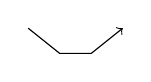
\begin{tikzpicture}[scale=0.4]
		\draw[->] (0, 0.8) -- (1, 0) -- (2, 0) -- (3, 0.8);
	\end{tikzpicture}
	的合成无关 $\Hom$ 集的加法结构, 仅涉及范畴中的有限积, 有限余积及其特例零对象, 以及它们带有的典范态射.
	
	对于 (iii), 回忆到所有有限积 (或有限余积) 皆可由零对象和双积 $\oplus$ 来构造.

	若 $(F, G)$ 为伴随对, 则 $F$ 保 $\varinjlim$ 而 $G$ 保 $\varprojlim$, 见 \cite[定理 2.8.12]{Li1}; 另一方面, 等价保所有极限. 因此 (iv) 和 (v) 都是 (ii) 的特例.
\end{proof}

事实上, 命题 \ref{prop:additive-cat-addition} 对加法的描述表明加性范畴 $\mathcal{C}$ 的``加性''乃是范畴 $\mathcal{C}$ 的一种性质, 而非额外的结构.

\begin{definition}
	\index{he@核 (kernel)} \index[sym1]{kerf@$\Ker(f)$}
	\index{yuhe@余核 (cokernel)}\index[sym1]{cokerf@$\Coker(f)$}
	设 $\mathcal{C}$ 为具有零对象的 $\cate{Ab}$-范畴, $f: X \to Y$ 为 $\mathcal{C}$ 中的态射.
	\begin{itemize}
		\item 若等化子 $\Ker(f,0)$ 存在, 则称 $\Ker(f) := \Ker(f,0)$ 连同 $\Ker(f) \hookrightarrow X$ 为 $f$ 的\emph{核}.
		\item 若余等化子 $\Coker(f,0)$ 存在, 则称 $\Coker(f) := \Coker(f,0)$ 连同 $Y \twoheadrightarrow \Coker(f)$ 为 $f$ 的\emph{余核}.
	\end{itemize}
	特别地, $\Ker(f) \to X \to Y$ 和 $X \to Y \to \Coker(f)$ 的合成按定义都是 $0$.
\end{definition}

对核以及余核, 可以有几种互补的视角.
\begin{itemize}
	\item 先考虑 $\Ker(f)$. 对任意态射 $g: T \to X$, 既然 $T \xrightarrow{g} X \xrightarrow{0} Y$ 的合成必为 $0$, 于是 $\Ker(f) = \Ker(f,0)$ 作为等化子的泛性质可表述为交换图表:
	\[\begin{tikzcd}
		& T \arrow[dashrightarrow, ld, "{\exists! g'}"'] \arrow[d, "g"] \arrow[rd, "0"] & \\
		\Ker(f) \arrow[r] & X \arrow[r, "f"'] & Y .
	\end{tikzcd}\]
	\item 考虑 $\Coker(f)$. 对任意态射 $h: Y \to T$, 既然 $X \xrightarrow{0} Y \xrightarrow{h} T$ 的合成必为 $0$. 于是 $\Coker(f) = \Coker(f, 0)$ 作为余等化子的泛性质可表述为交换图表:
	\[\begin{tikzcd}
		X \arrow[r, "f"] \arrow[rd, "0"'] & Y \arrow[r] \arrow[d, "h"] & \Coker(f) \arrow[dashrightarrow, ld, "{\exists! h'}"] . \\
		& T &
	\end{tikzcd}\]
	\item 以上两者显然相互对偶: $\Coker(f) = \Ker(f^{\opp})$, $\Ker(f) = \Coker(f^{\opp})$.
\end{itemize}

由于通过零对象分解的态射正是 $0$, 泛性质也有基于拉回和推出图表的刻画, 请读者疾速验证:
\begin{equation}\label{eqn:Ker-Coker-triangles}
	\begin{tikzcd}
		\Ker(f) \arrow[phantom, r, "\simeq" description] & X \dtimes{Y} 0 \arrow[r] \arrow[d] \arrow[phantom, rd, "\Box" description] & X \arrow[d, "f"] \\
		& 0 \arrow[r] & Y
	\end{tikzcd} \qquad \begin{tikzcd}
		X \arrow[r, "f"] \arrow[d] & Y \arrow[d] & \\
		0 \arrow[r] & Y \dsqcup{X} 0 \arrow[phantom, lu, "\boxplus" description] & \Coker(f) \arrow[phantom, l, "\simeq" description] .
\end{tikzcd}\end{equation}

\begin{remark}\label{rem:equalizer-Ker}
	一般的等化子 $\Ker(f,g)$ 可以化约到上述的核: 考虑态射
	\[\begin{tikzcd}
	T \arrow[r, "h"] & X \arrow[r, yshift=0.2em, "f"] \arrow[r, yshift=-0.2em, "g"'] & Y
	\end{tikzcd}, \]
	条件 $fh = gh$ 等价于 $(f-g)h = 0$, 由此立得 $\Ker(f,g) = \Ker(f-g, 0) =: \Ker(f-g)$. 对偶地, $\Coker(f,g) = \Coker(f-g,0) =: \Coker(f-g)$.
\end{remark}

今后主要考虑 $\mathcal{C}$ 为加性范畴的情形.

\begin{proposition}\label{prop:Ker-Coker-composite}
	对于加性范畴 $\mathcal{C}$ 中的态射 $X \xrightarrow{f} Y \xrightarrow{g} Z$, 存在交换图表
	\[\begin{tikzcd}[row sep=small, column sep=small]
		\Ker(gf) \arrow[rr, "\sim"] \arrow[hookrightarrow, rd] & & X \dtimes{Y} \Ker(g) \arrow[hookrightarrow, ld] \\
		& X &
	\end{tikzcd} \quad \begin{tikzcd}[row sep=small, column sep=small]
		Z \dsqcup{Y} \Coker(f) \arrow[rr, "\sim"] & & \Coker(gf) \\
		& Z \arrow[twoheadrightarrow, lu] \arrow[twoheadrightarrow, ru] &
	\end{tikzcd}\]
	其中 $X \dtimes{Y} \Ker(g) \to X$ (或 $Z \to Z \dsqcup{Y} \Coker(f)$) 是纤维积 (或余积) 自带的典范态射, 前提是所论的 $\Ker$, $\Coker$ 和极限皆存在.
\end{proposition}
\begin{proof}
	基于 \eqref{eqn:Ker-Coker-triangles}, 分段作纤维积得典范同构 $\Ker(gf) \simeq X \dtimes{Z} 0 \simeq X \dtimes{Y} (Y \dtimes{Z} 0) \simeq X \dtimes{Y} \Ker(g)$. 对偶性给出 $\Coker(gf)$ 的情形.
\end{proof}

等化子及余等化子的函子性诱导核及余核的函子性, 以交换图表刻画为
\begin{equation}\label{eqn:Ker-Coker-functoriality}\begin{tikzcd}
		\Ker(f) \arrow[r] \arrow[dashrightarrow, d, "\exists!"'] & X \arrow[d, "a"'] \arrow[r, "f"] & Y \arrow[d, "b"] \\
		\Ker(g) \arrow[r] & X' \arrow[r, "g"'] & Y'
	\end{tikzcd} \qquad \begin{tikzcd}
		X \arrow[d, "a"'] \arrow[r, "f"] & Y \arrow[d, "b"] \arrow[r] & \Coker(f) \arrow[dashrightarrow, d, "\exists!"'] \\
		X' \arrow[r, "g"'] & Y' \arrow[r] & \Coker(g) .
\end{tikzcd}\end{equation}

以下结果说明拉回 (或推出) 保核 (或余核).
\begin{proposition}\label{prop:pull-back-ker}
	若加性范畴 $\mathcal{C}$ 中的图表
	\[\begin{tikzcd}
		X \arrow[r, "f"] \arrow[d, "a"'] & Y \arrow[d, "b"] \\
		X' \arrow[r, "g"'] & Y'
	\end{tikzcd}\]
	是拉回 (或推出) 图表, 则 \eqref{eqn:Ker-Coker-functoriality} 的态射 $\Ker(f) \to \Ker(g)$ (或 $\Coker(f) \to \Coker(g)$) 为同构, 前提是所论的 $\Ker$ 和 $\Coker$ 存在.
\end{proposition}
\begin{proof}
	对偶性将论证归结为拉回的情形. 对任意对象 $T$, 由泛性质可以验证
	\begin{align*}
		\Hom(T, \Ker(f)) & \simeq \Ker\left[ \Hom(T, X) \to \Hom(T, Y) \right] \\
		& \simeq \Ker\left[ \Hom(T, Y) \dtimes{\Hom(T, Y')} \Hom(T, X') \to \Hom(T, Y) \right] \\
		& = \Ker\left[ \Hom(T, X') \to \Hom(T, Y') \right] \simeq \Hom(T, \Ker(g)),
	\end{align*}
	其中每个箭头都是典范的. 米田引理遂蕴涵 $\Ker(f) \rightiso \Ker(g)$; 详见定理 \ref{prop:Yoneda} 的回顾.
\end{proof}

\begin{lemma}\label{prop:mono-epi-ker-coker}
	设 $\mathcal{C}$ 为加性范畴, $f: X \to Y$ 为 $\mathcal{C}$ 中的态射, 则:
	\begin{enumerate}[(i)]
		\item $f$ 是单态射 (或满态射) 当且仅当 $\Ker(f) = 0$ (或 $\Coker(f) = 0$);
		\item $f$ 是零态射等价于 $\Ker(f) \rightiso X$, 也等价于 $Y \rightiso \Coker(f)$;
		\item 给定 $k: Y \to Z$ (或 $k': W \to X$), 存在唯一的交换图表如下:
		\[\begin{tikzcd}[row sep=small, column sep=small]
		\Ker(kf) \arrow[rd] & & \Ker(f) \arrow[ld] \arrow[hookrightarrow, ll, "\exists !"'] \\
		& X &
		\end{tikzcd} \quad \text{或} \quad
		\begin{tikzcd}[row sep=small, column sep=small]
		\Coker(fk') \arrow[twoheadrightarrow, rr, "\exists !"] & & \Coker(f) \\
		& Y \arrow[lu] \arrow[ru] &
		\end{tikzcd}\]
		前提是所论的核 (或余核) 存在. 若 $k$ 单 (或 $k'$ 满), 则 $\Ker(f) \rightiso \Ker(kf)$ (或 $\Coker(fk') \rightiso \Coker(f)$).
	\end{enumerate}
\end{lemma}
\begin{proof}
	先考虑 (i). 基于对偶性, 仅需处理单态射情形. 按定义, $f$ 为单态射等价于对任一对态射 $g_1, g_2: T \to X$ 都有 $f(g_1 - g_2) = 0 \iff g_1 - g_2 = 0$. 这相当于说对任意 $g: T \to X$, 下式成立: $f g = 0$ 当且仅当 $g$ 分解为 $T \to 0 \to X$. 这无非是说零对象符合 $\Ker(f)$ 的泛性质.
	
	同理, 对 (ii) 证 $f = 0 \iff \Ker(f) \rightiso X$ 即可. 然而 $\Ker(f) = \Ker(f, 0)$, 所求的等价容易归结为等化子的定义.
	
	至于 (iii), 同样仅考虑 $\Ker$ 的情形,
	\[\begin{tikzcd}[column sep=small]
		\left\{ g \in \Hom(T, X): fg=0 \right\} \arrow[phantom, r, "\subset" description] & \left\{ g \in \Hom(T, X): kfg=0 \right\} \\
		\Hom(T, \Ker(f)) \arrow[u, "1:1"] & \Hom(T, \Ker(kf)) \arrow[u, "1:1"']
	\end{tikzcd}\]
	当 $k$ 单时第一行取等号. 应用米田引理以完成证明.
\end{proof}

在加性范畴中, 定义 \ref{def:Im-Coim} 介绍的像和余像有简单的描述.

\begin{proposition}\label{prop:Im-Coim-additive}
	\index{xiang}\index{yuxiang}\index[sym1]{imf} \index[sym1]{coimf}
	设 $f: X \to Y$ 为加性范畴 $\mathcal{C}$ 中的态射, 则有典范同构
	\begin{align*}
		\Image(f) & \simeq \Ker\left[ Y \to \Coker(f) \right] \hookrightarrow Y, \\
		\Coim(f) & \simeq \Coker\left[ \Ker(f) \to X \right] \twoheadleftarrow X ;
	\end{align*}
	前提是所论的核, 余核皆存在.
\end{proposition}
\begin{proof}
	基于对偶性, 以下仅考虑 $\Image(f)$. 考虑典范态射 $i_1, i_2: Y \to Y \dsqcup{X} Y$. 应用米田引理, 问题化为对所有 $T \in \Obj(\mathcal{C})$ 验证
	\begin{multline*}
		\Hom\left( T, \Image(f) \right) = \left\{ h: T \to Y \;\middle|\; i_1 h = i_2 h \right\} \\
		= \left\{ \begin{array}{r|l}
			h: T \to Y & \forall S \in \Obj(\mathcal{C}),\; \forall s_1, s_2: Y \to S, \\
			& s_1 f = s_2 f \implies s_1 h = s_2 h
		\end{array}\right\} \\
		\xlongequal{s := s_1 - s_2} \left\{ \begin{array}{r|l}
			h: T \to Y & \forall S \in \Obj(\mathcal{C}),\; \forall s: Y \to S, \\
			& s f = 0 \implies sh = 0
		\end{array}\right\} \\
		= \left\{ \begin{array}{r|l}
			h: T \to Y & T \xrightarrow{h} Y \twoheadrightarrow \Coker(f) \\
			& \text{合成为}\; 0
		\end{array}\right\}
		\leftiso \Hom\left( T, \Ker\left[ Y \to \Coker(f) \right] \right).
	\end{multline*}
	以上第一个等式缘于 $\Image(f) := \Ker(i_1, i_2)$. 对于第二个等式, 先将 $h$ 的条件改写为对所有 $s': Y \dsqcup{X} Y \to S$ 皆有 $s' i_1 h = s' i_2 h$, 再用纤维余积的泛性质
	\begin{align*}
		\Hom\left( Y \dsqcup{X} Y, S \right) & \xrightarrow{1:1} \Hom(Y,S) \dtimes{\Hom(X,S)} \Hom(Y,S) \\
		s' & \longmapsto \left( s' i_1, s' i_2 \right) =: (s_1, s_2).
	\end{align*}
	第四个等式是按余核泛性质化简到 $S = \Coker(f)$ 的产物.
\end{proof}

最简单的例子是当 $f$ 为零态射时, 引理 \ref{prop:mono-epi-ker-coker} (ii) 蕴涵 $\Image(f) = 0 = \Coim(f)$.

\begin{example}\label{eg:strict-morphism}
	承接例 \ref{eg:additive-category} 的讨论. 考虑范畴 $R\dcate{Mod}$. 模同态 $f: A \to B$ 总有核以及余核, 按经典方式取为 $\Ker(f) = f^{-1}(0)$ 以及 $\Coker(f) = B/\{f(a) : a \in A\}$. 据定义立见 $\Image(f)$ 是 $f$ 在集合论意义下的像, $\Coim(f) = A/\Ker(f)$, 而 \eqref{eqn:strict-morphism} 中的典范态射 $\Coim(f) \to \Image(f)$ 无非是模论里的典范同构 $A/\Ker(f) \rightiso \Image(f)$. 因此 $R\dcate{Mod}$ 中所有态射皆严格.
	
	接着考虑例 \ref{eg:additive-category} 的加性范畴 $\cate{Ban}_{\CC}$. 连续线性映射 $f: X \to Y$ 的核是寻常的 $\Ker(f) = f^{-1}(0)$, 仍是 Banach 空间; 另一方面, $\Coker(f) = Y/\overline{\left\{ f(x): x \in X \right\}}$ 带有商范数. 对之 \eqref{eqn:strict-morphism} 的态射化为
	\[\begin{tikzcd}[row sep=small, column sep=small]
	\Coim(f) \arrow[equal, r] & X/f^{-1}(0) \arrow[r] & \overline{\left\{ f(x): x \in X \right\}} \arrow[equal, r] & \Image(f) \\
	& x + f^{-1}(0) \arrow[mapsto, r] \arrow[phantom, u, "\in" description, sloped] & f(x) \arrow[phantom, u, "\in" description, sloped] &
	\end{tikzcd}\]
	右边带诱导自 $Y$ 的拓扑, 左边则带 $X$ 的商拓扑. 设 $f: X \to Y$ 为 Banach 空间之间的连续线性单射, $f$ 像稠密而非满, 此时 $\Coim(f) = X \to Y = \Image(f)$ 非同构, 因而 $\cate{Ban}_{\CC}$ 中存在非严格的态射.
\end{example}

\section{推广: 交换环上的线性范畴}\label{sec:linear-cat}
加性范畴的 $\Hom$ 集具有加法群的结构, 而在许多情景中, $\Hom$ 集还进一步带有来自某个交换环 $\Bbbk$ 的纯量乘法. 例如在 $\Bbbk\dcate{Mod}$ 中, 每个 $\Hom$ 集自然地都是 $\Bbbk$-模, 而态射的合成是 $\Bbbk$-双线性的.

\begin{definition}\label{def:cat-k-linear}
	\index{fanchou!$\Bbbk\dcate{Mod}$-}
	\index{hanzi!$\Bbbk$-线性 ($\Bbbk$-linear)}
	设 $\Bbbk$ 为交换环. 若范畴 $\mathcal{A}$ 中的 $\Hom$ 集都带有 $\Bbbk$-模结构, 使得态射合成 $\Hom(Y, Z) \times \Hom(X, Y) \to \Hom(X, Z)$ 对所有对象 $X, Y, Z$ 都是 $\Bbbk$-双线性映射, 或者换言之有交换图表
	\[\begin{tikzcd}
		\Hom(Y, Z) \times \Hom(X, Y) \arrow[d] \arrow[r, "\text{合成}"] & \Hom(X, Z) \\
		\Hom(Y, Z) \dotimes{\Bbbk} \Hom(X, Y) \arrow[ru, bend right, start anchor=east, "{\exists! \; \text{$\Bbbk$-模同态}}"']
	\end{tikzcd}  \]
	则称 $\mathcal{A}$ 同这些资料成为 $\Bbbk\dcate{Mod}$-范畴.

	设 $F: \mathcal{A} \to \mathcal{A}'$ 为 $\Bbbk\dcate{Mod}$-范畴之间的函子, 若 $\Hom(X, Y) \to \Hom(FX, FY)$ 对所有 $X, Y \in \Obj(\mathcal{A})$ 都是 $\Bbbk$-模同态, 则称 $F$ 是 $\Bbbk$-线性函子.
\end{definition}

注意到 $\Bbbk\dcate{Mod}$ 对张量积 $\otimes := \dotimes{\Bbbk}$ 成为幺半范畴, 因此 $\Bbbk\dcate{Mod}$-范畴这一称呼和 \cite[\S 3.4]{Li1} 中关于充实范畴的术语一致. 先前介绍的 $\cate{Ab}$-范畴即 $\Z\dcate{Mod}$-范畴; 相反地, 忘却 $\Bbbk\dcate{Mod}$-范畴上的纯量乘法, 就得到 $\cate{Ab}$-范畴.

\begin{example}
	仅有一个对象的 $\Bbbk\dcate{Mod}$-范畴无非是 $\Bbbk$-代数, 对应由 $\mathcal{A} \mapsto \End_{\mathcal{A}}(\star)$ 给出, 此处 $\Obj(\mathcal{A}) = \{\star\}$.
\end{example}

命题 \ref{prop:automatic-Ab-morphism} 的论证原封不动地照搬, 给出以下结果.

\begin{proposition}\label{prop:automatic-k-morphism}
	设 $\mathcal{A}$ 和 $\mathcal{A}'$ 是 $\Bbbk\dcate{Mod}$-范畴.
	\begin{enumerate}
		\item 给定一对伴随函子
		$\begin{tikzcd}
			F: \mathcal{A} \arrow[shift left, r] & \mathcal{A}' \arrow[shift left, l] : G
		\end{tikzcd}$,
		其中 $F$, $G$ 皆是 $\Bbbk$-线性的, 则伴随同构 $\Hom_{\mathcal{A}'}(F(\cdot), \cdot) \rightiso \Hom_{\mathcal{A}}(\cdot, G(\cdot))$ 是 $\Bbbk$-线性的.
		\item 对于任意 $\alpha: I \to \mathcal{A}$, 双射
		\[ \Hom_{\mathcal{A}}\left( \varinjlim \alpha, T \right) \simeq \varprojlim_{i \in \Obj(I)} \Hom_{\mathcal{A}}(\alpha(i), T), \quad T \in \Obj(\mathcal{A}) \]
		是 $\Bbbk$-线性的, 前提是极限存在. 对 $\varprojlim$ 亦同.
	\end{enumerate}
\end{proposition}

如无另外申明, 今后 $\Bbbk\dcate{Mod}$-范畴之间的函子和等价都默认为 $\Bbbk$-线性的.

\begin{definition}\label{def:k-linear-cat}
	\index{fanchou!$\Bbbk$-线性 ($\Bbbk$-linear)}
	若给定的加性范畴 $\mathcal{A}$ 带有 $\Bbbk$-线性结构, 与原有的 $\cate{Ab}$-结构相容, 则称此资料为 $\Bbbk$-线性范畴.
\end{definition}

这相当于在 \S\ref{sec:Ker-Coker} 的讨论中以 $\Bbbk\dcate{Mod}$-范畴替代 $\cate{Ab}$-范畴. 本章关于加性范畴的结果多数能扩及 $\Bbbk$-线性的情形, 论证并无二致. 唯一的例外关乎推论 \ref{prop:automatic-additivity}: 在加性范畴中, $\Hom$ 集的加法能由范畴本身的性质来刻画, 但论及 $\Bbbk$-纯量乘法则不然; 相应地, $\Bbbk$-线性范畴之间的函子 (乃至于等价) 没有自动成为 $\Bbbk$-线性的理由.

以下搜集关于 $\Bbbk$-线性的几则结果. 回顾任意范畴 $\mathcal{A}$ 的\emph{中心}
\index{zhongxin@中心 (center)} \index[sym1]{ZA@$Z(\mathcal{A})$}
$Z(\mathcal{A}) := \End(\identity_{\mathcal{A}})$, 其元素是恒等函子 $\identity_{\mathcal{A}}$ 到自身的态射, 写作 $(a_X)_{X \in \Obj(\mathcal{A})}$, 其中 $a_X \in \End_{\mathcal{A}}(X)$. 中心对态射合成构成交换幺半群; 见 \cite[定义 2.3.8, 命题 2.3.9]{Li1}. 若 $\mathcal{A}$ 是 $\cate{Ab}$-范畴, 则 $Z(\mathcal{A})$ 相对于合成与加法 $(a_X)_X + (b_X)_X := (a_X + b_X)_X$ 成为交换环.

\begin{proposition}\label{prop:k-linear-center}
	设 $\mathcal{A}$ 为 $\cate{Ab}$-范畴, 则有双射
	\[ \left\{ \text{$\mathcal{A}$ 上的 $\Bbbk\dcate{Mod}$-范畴结构} \right\} \stackrel{1:1}{\longleftrightarrow} \Hom_{\text{环}}(\Bbbk, Z(\mathcal{A})). \]
	映法如下. 若指定了 $\mathcal{A}$ 上的 $\Bbbk\dcate{Mod}$-范畴结构, 对每个 $a \in \Bbbk$ 和 $X \in \Obj(\mathcal{A})$, 定义 $a_X := a \cdot \identity_X \in \End_{\mathcal{A}}(X)$, 则 $a \mapsto (a_X)_{X \in \Obj(\mathcal{A})} \in Z(\mathcal{A})$ 是环同态. 反之, 给定属于右式的环同态 $a \mapsto (a_X)_{X \in \Obj(\mathcal{A})}$, 以 $a \cdot f := f \circ a_X = a_Y \circ f$ 定义 $\mathcal{A}$ 上的 $\Bbbk\dcate{Mod}$-范畴结构, 其中 $f \in \Hom(X, Y)$.
\end{proposition}
\begin{proof}
	刻画 $(a_X)_{X \in \Obj(\mathcal{A})} \in Z(\mathcal{A})$ 的条件正是 $f \circ a_X = a_Y \circ f$, 其中 $f \in \Hom(X, Y)$ 任取. 若 $\mathcal{A}$ 带有 $\Bbbk\dcate{Mod}$-范畴结构, 命 $a_X := a \cdot \identity_X$, 则双线性蕴涵 $f \circ a_X = f \circ (a \cdot \identity_X) = (a f) \circ \identity_X = (a \cdot \identity_Y) \circ f = a_Y \circ f$, 故 $(a_X)_{X \in \Obj(\mathcal{A})} \in Z(\mathcal{A})$. 其余验证是平凡的.
\end{proof}

作为推论, $\cate{Ab}$-范畴 $\mathcal{A}$ 自然地成为 $Z(\mathcal{A})\dcate{Mod}$-范畴.

\section{由函子观极限}\label{sec:limit-functor}
函子 $F: \mathcal{C} \to \mathcal{D}$ 和极限间的种种关系大致可以分成两个方向. 以 $\varinjlim$ 为例, 给定函子 $\alpha: I \to \mathcal{C}$, 试问:
\begin{itemize}
	\item 设 $\varinjlim \alpha$ 存在, 其像 $F\left(\varinjlim \alpha\right)$ 是否给出 $\varinjlim (F\alpha)$?
	\item 设 $\varinjlim F\alpha$ 存在, 它能否``提升''到 $\mathcal{C}$ 上? 此提升在何种意义下唯一?
\end{itemize}

此处主要讨论 $\varinjlim$ 的情形; 这些结果对于 $\varprojlim$ 当然也有对应的版本; 鉴于对偶性, 细节不必重复.

我们以锥和范畴 $(\alpha/\Delta)$ 的语言来梳理 $\varinjlim$.

\begin{convention}\label{con:limit-cone}
	相对于给定的函子 $\alpha: I \to \mathcal{C}$, 称 $\mathcal{C}$ 中满足下述条件的资料 $(L, (f_i)_{i \in \Obj(I)})$ 为以 $\alpha$ 为底, 以 $L$ 为顶点的\emph{锥}:
	\begin{compactitem}
		\item $L$ 是 $\mathcal{C}$ 的对象,
		\item 每个 $f_i : \alpha(i) \to L$ 都是 $\mathcal{C}$ 的态射, 具备相容性条件 $f_j \circ \alpha(i \to j) = f_i$, 其中 $[i \to j]$ 取遍 $\mathrm{Mor}(I)$.
	\end{compactitem}
\end{convention}

按 \cite[\S 2.7]{Li1} 的语言, 这些锥构成范畴\footnote{此处 $\Delta$ 的严格含义是对角函子 $\mathcal{C} \to \mathcal{C}^I$, 见例 \ref{eg:comma-vs-cone}, 按拼音命名. 但也无妨按照象形原则将 $\Delta$ 想成``锥'', 见图 \eqref{eqn:injlim-diagram}.} $(\alpha / \Delta)$; 具体地说, 当底 $\alpha$ 固定, 从锥 $(L, (f_i)_i)$ 到锥 $(M, (g_i)_i)$ 的态射是交换图表
\begin{equation}\label{eqn:injlim-diagram}\begin{tikzcd}
	& L \arrow[d] & \\
	\alpha(i) \arrow[bend right, rr, "\alpha(i \to j)"'] \arrow[r, "g_i"] \arrow[ru, "f_i"] & M & \alpha(j) \arrow[l, "{g_j}"'] \arrow[lu, "f_j"']
\end{tikzcd}\end{equation}
其中 $i \to j$ 取遍 $\Mor(I)$, 态射合成按明显的方式操作. 按定义, $\varinjlim \alpha$ 连同其自带的典范态射族 $\iota_i: \alpha(i) \to \varinjlim \alpha$ 是 $(\alpha / \Delta)$ 的始对象.
\index{jixian}\index[sym1]{lim}

函子 $F$ 按自明的方式诱导函子 $(\alpha/\Delta) \to (F\alpha / \Delta)$, 映锥 $(L, (f_i)_i)$ 为 $(FL, (Ff_i)_i)$. 设 $\varinjlim \alpha$ 存在, 倘若 $\varinjlim F\alpha$ 也存在, 则在 $(F\alpha / \Delta)$ 中存在唯一态射
\[ \varinjlim F\alpha \to F(\varinjlim \alpha), \]
它是同构当且仅当 $\left( F(\varinjlim \alpha), (F\iota_i)_i \right)$ 给出 $\varinjlim F\alpha$.

倒转箭头, $\varprojlim \alpha$ 可刻画为 $(\Delta/\alpha)$ 的终对象. 在所论 $\varprojlim$ 存在的前提下, 在 $(\Delta/F\alpha)$ 中存在唯一态射
\[ F\varprojlim \alpha \to \varprojlim F\alpha. \]

\begin{definition}\label{def:create-limit}
	\index{jixian!保, 返, 生 (preserve, reflect, create)}
	给定 $F: \mathcal{C} \to \mathcal{D}$ 和函子 $\alpha: I \to \mathcal{C}$, 考虑锥范畴之间的函子 $(\alpha/\Delta) \to (F\alpha/\Delta)$.
	\begin{itemize}
		\item 称 $F$ \emph{保}此 $\varinjlim$, 如果 $(\alpha/\Delta) \to (F\alpha/\Delta)$ 映始对象 (假如存在) 为始对象.
		\item 称 $F$ \emph{返}此 $\varinjlim$, 如果仅 $(\alpha/\Delta)$ 的始对象 (假如存在) 方能被映为 $(F\alpha/\Delta)$ 的始对象.
		\item 称 $F$ \emph{生}此 $\varinjlim$, 如果
		\begin{compactitem}
			\item $\varinjlim F\alpha \;\text{存在} \implies \varinjlim \alpha \;\text{存在}$;
			\item $F$ 保此 $\varinjlim$, 返此 $\varinjlim$.
		\end{compactitem}
	\end{itemize}
	对于 $\varprojlim$ 同样有相应的概念, 以 $\mathcal{C}^{\opp}$ 和 $\mathcal{D}^{\opp}$ 代 $\mathcal{C}$ 和 $\mathcal{D}$ 即可相互过渡.
\end{definition}

注意: 这些概念系于所论的 $\alpha$, 比如 $F$ 完全有可能保有限的 $\varinjlim$ 而不保一般的 $\varinjlim$.

给定 $\alpha$, 函子生 $\varinjlim$ (或 $\varprojlim$) 相当于说 $\mathcal{D}$ 中定义此极限的锥可以唯一地提升到 $\mathcal{C}$, 并且使后者给出 $\mathcal{C}$ 中相应的极限; 唯一性来自定义中关于返 $\varinjlim$ (或 $\varprojlim$) 的条件. 这一观点将在稍后的例 \ref{eg:Grp-Set-create} 和命题 \ref{prop:forget-create} 中清楚呈现. 

\begin{proposition}\label{prop:ff-reflect}
	全忠实函子返一切 $\varinjlim$ 和 $\varprojlim$.
\end{proposition}
\begin{proof}
	以 $\varinjlim$ 为例. 设 $F$ 全忠实, 则 $(\alpha/\Delta)$ 的始对象的泛性质可在取 $F$ 后在 $(F\alpha/\Delta)$ 中验证.
\end{proof}

顺势引入一个方便的概念.
\begin{definition}\label{def:conservative}
	\index{hanzi!保守 (conservative)}
	满足以下条件的函子 $F$ 称为\emph{保守}的: 态射 $f \in \Mor(\mathcal{C})$ 为同构当且仅当 $Ff \in \Mor(\mathcal{D})$ 为同构. 
\end{definition}

\begin{remark}\label{rem:conservative-reflect}
	若 $F$ 是保守函子, 则只要 $\varinjlim \alpha$ 存在, 而且 $F$ 保此 $\varinjlim$, 则 $F$ 也必然返此 $\varinjlim$. 缘由如下: 设 $L \in \Obj((\alpha/\Delta))$ 被映为 $(F\alpha/\Delta)$ 的始对象; 考虑 $(\alpha/\Delta)$ 中的唯一态射 $\varinjlim \alpha \to L$, 由于 $F$ 保此 $\varinjlim$, 它在 $F$ 之下的像必为同构, 从而保守条件确保 $\varinjlim \alpha \to L$ 也是同构.
	
	在此前提下, 关于 $F$ 生 $\varinjlim$ 的定义中可以去除返 $\varinjlim$ 的条件.
\end{remark}

\begin{example}\label{eg:Grp-Set-create}
	以下来验证从群范畴 $\cate{Grp}$ 到集合范畴 $\cate{Set}$ 的忘却函子 $U$ 生所有小 $\varprojlim$.
	
	这是 $\varprojlim$ 在 $\cate{Grp}$ 和 $\cate{Set}$ 中的具体构造的推论, 见 \cite[例 2.7.5 和 2.8.7]{Li1}. 详言之, 取小范畴 $I$ 和函子 $\beta: I^{\opp} \to \cate{Grp}$. 作为集合,
	\[ \varprojlim U\beta = \left\{\begin{array}{r|l}
		(x_i)_i \in \prod_{i \in \Obj(I)} U\beta(i) & \forall [i \to j] \in \mathrm{Mor}(I), \\
		& \beta(i \to j)(x_j) = x_i
	\end{array}\right\}, \]
	投影 $p_i: \varprojlim U\beta \to U\beta(i)$ 映 $(x_j)_j$ 为 $x_i$. 眼下的任务是:
	\begin{enumerate}
		\item 赋予 $\varprojlim U\beta$ 群结构, 使得每个 $p_i$ 都是群同态, 并说明这样的群结构唯一;
		\item 对此群连同投影同态族 $(p_i)_i$ 验证 $\varprojlim \beta$ 的泛性质. 
	\end{enumerate}

	显然 $\varprojlim U\beta$ 是直积 $\prod_i \beta(i)$ 的子群, 记为 $\varprojlim \beta \in \Obj(\cate{Grp})$, 这是使每个 $p_i$ 皆为群同态的唯一群结构. 这就完成了第一点.
	
	接着对锥 $\left( \varprojlim \beta, (p_i)_i\right)$ 验证泛性质. 考虑 $\cate{Grp}$ 中任意的锥 $(L, (q_i)_i)$, 其中 $q_i: L \to \beta(i)$. 泛性质给出唯一的映射 $\varphi: UL \to \varprojlim U\beta$ 使得 $p_i \varphi = q_i$ 恒成立. 事实上 $\varphi$ 具体写作 $y \mapsto (q_i(y))_{i \in \Obj(I)}$, 故它升级为群同态 $L \to \varinjlim \beta$. 验证完毕.
\end{example}

基于完全类似的论证, 可以说明从紧 Hausdorff 空间范畴 $\cate{CHaus}$ 到 $\cate{Set}$ 的忘却函子也生所有小 $\varprojlim$. 相关验证属于本章习题.

次一则结果涉及形如 $\mathcal{C}^J$ 的函子范畴 (可能是``大''范畴, 但无妨), 这需要两步准备.

\begin{itemize}
	\item 设 $J$ 为集合, $J$ 份 $\mathcal{C}$ 的积 $\mathcal{C}^J$ 定义为: $\Obj\left(\mathcal{C}^J\right) = \Obj(\mathcal{C})^J$, $\mathrm{Mor}\left(\mathcal{C}^J \right) = \mathrm{Mor}(\mathcal{C})^J$. 对每个 $j \in J$ 皆有自明的投影函子 $p_j: \mathcal{C}^J \to \mathcal{C}$.

	给定范畴 $I$ 和函子 $\alpha: I \to \mathcal{C}^J$, 若对对每个 $j$ 都存在 $\varinjlim (p_j \alpha)$, 则 $\varinjlim \alpha$ 也存在, 其构造方式是``逐点''或曰``逐对象''地取极限: $\varinjlim \alpha = \left( \varinjlim (p_j \alpha) \right)_{j \in J}$.

	\item 设 $J$ 为范畴, 对之可考虑函子范畴 $\mathcal{C}^J$. 对每个 $j \in \Obj(J)$ 都有求值函子 $\mathrm{ev}_j: \mathcal{C}^J \to \mathcal{C}$, 映对象 $F$ 为 $Fj$, 映态射 $\varphi = (\varphi_{j'})_{j' \in \Obj(J)}$ 为 $\varphi_j$. 稍后将考虑形如 $\alpha: I \to \mathcal{C}^J$ 的函子及其 $\varinjlim$; 注意到 $\alpha$ 可视同函子 $I \times J \to \mathcal{C}$, 取值写作 $\alpha(i, j)$.
\end{itemize}

两套符号是兼容的: 若 $J$ 是离散范畴, 视之为集合, 则 $\mathcal{C}^J$ 无非是先前讨论的积. 对于一般的 $J$, 忘却函子 $\mathcal{F}: \mathcal{C}^J \to \mathcal{C}^{\Obj(J)}$ 映对象 $F$ 为 $(Fj)_{j \in \Obj(J)}$, 映态射 $\varphi$ 为 $(\varphi_j)_{j \in \Obj(J)}$. 因此 $\mathrm{ev}_j = p_j \mathcal{F}$.

\begin{proposition}\label{prop:forget-create}
	设 $J$ 和 $\mathcal{C}$ 为范畴.
	\begin{enumerate}[(i)]
		\item 忘却函子 $\mathcal{F}: \mathcal{C}^J \to \mathcal{C}^{\Obj(J)}$ 生 $\varinjlim$ 和 $\varprojlim$.
		\item 设 $I$ 为范畴, 而且所有始自 $I$ 的函子在 $\mathcal{C}$ 中皆有 $\varinjlim$ (或 $\varprojlim$), 则所有形如 $I \to \mathcal{C}^J$ 的函子在 $\mathcal{C}^J$ 中也有 $\varinjlim$ (或 $\varprojlim$).
		\item 承上, 对每个 $j \in \Obj(J)$, 求值函子 $\mathrm{ev}_j: \mathcal{C}^J \to \mathcal{C}$ 保这些 $I$ 给出的 $\varinjlim$ (或 $\varprojlim$); 换言之, $\mathcal{C}^J$ 中的极限也是``逐点''或逐对象地定义的.
	\end{enumerate}
\end{proposition}
\begin{proof}
	考虑 $\varinjlim$ 情形即可. 对于 (i), 选定 $\alpha: I \to \mathcal{C}^J$, 假设 $\varinjlim \mathcal{F}\alpha$ 存在, 由锥
	\[ \left( (X(j))_{j \in \Obj(J)}, \; \left( \iota_i = (\iota_{i, j})_{j \in \Obj(J)} \right)_{i \in \Obj(I)} \right) \]
	给出, 其中 $\iota_{i,j}: \alpha(i, j) \to X(j)$. 我们希望将它提升为 $\mathcal{C}^J$ 中的锥, 使之给出 $\varinjlim \alpha$.
	
	首先观察对所有 $j$ 必有 $X(j) = \varinjlim \alpha(\cdot, j)$. 对于所有态射 $j \to j'$, 极限的函子性 (见 \cite[引理 2.7.4]{Li1}) 遂给出唯一的态射 $X(j \to j'): X(j) \to X(j')$ 使下图交换
	\[\begin{tikzcd}
		\alpha(i, j) \arrow[r] \arrow[d, "{\iota_{i, j}}"'] & \alpha(i, j') \arrow[d, "{\iota_{i, j'}}"] \\
		X(j) \arrow[r, "{X(j \to j')}"'] & X(j')
	\end{tikzcd} \quad i \in \Obj(I). \]
	依此升级 $j \mapsto X(j)$ 为函子 $X: J \to \mathcal{C}$, 升级 $\iota_i: \alpha(i, \cdot) \to X$ 为 $\mathcal{C}^J$ 的态射. 不难验证 $(X, (\iota_i)_i) \in \Obj(\alpha/\Delta)$, 以下验证它是始对象. 由于函子 $\mathcal{F}$ 保守, 返 $\varinjlim$ 的条件不用再验证.

	给定 $(L, (f_i)_i) \in \Obj(\alpha/\Delta)$, 由 $\varinjlim \mathcal{F}\alpha$ 的泛性质确定唯一的态射 $\varphi = (\varphi_j)_j : \mathcal{F}X \to \mathcal{F}L$, 使下图三角部分对所有 $(i, j)$ 交换:
	\[\begin{tikzcd}
		& X(j) \arrow[d, "\varphi_j"] \arrow[r, "{X(j \to j')}" inner sep=0.8em] & X(j') \arrow[d, "\varphi_{j'}"] \\
		\alpha(i, j) \arrow[ru, "{\iota_{i,j}}"] \arrow[r, "f_{i, j}"' inner sep=0.8em] & L(j) \arrow[r, "{L(j \to j')}"' inner sep=0.8em] & L(j')
	\end{tikzcd}\]
	若能说明方块对所有 $j \to j'$ 皆交换, 则 $\varphi$ 升级为 $X \to L$. 外框已知交换, 故
	\[ \varphi_{j'} X(j \to j') \iota_{i, j} = L(j \to j') f_{i, j} = L(j \to j') \varphi_j \iota_{i, j} \]
	对所有 $i$ 成立; 始自 $X(j)$ 的态射由它和所有 $\iota_{i,j}$ 的合成确定, 故方块交换.

	至于 (ii), 考虑函子 $\alpha: I \to \mathcal{C}^J$. 根据此前讨论, $\mathcal{F}\alpha: I \to \mathcal{C}^{\Obj(J)}$ 有 $\varinjlim$, 它是逐对象地定义的. 由 (i) 可在 $\mathcal{C}$ 中生出 $\varinjlim \alpha$, 而关于 $\mathrm{ev}_j$ 保这些 $\varinjlim$ 的断言 (iii) 则是构造的直接结论.
\end{proof}

\section{滤过归纳极限}\label{sec:filtered-indlim}
数学分析的一则常识是数列的极限可以由任何子数列来计算, 这点在范畴论中体现为共尾的概念. 我们先从连通性切入.

\begin{definition}\index{fanchou!连通 (connected)}
	设 $I$ 为任意范畴, 若 $\Obj(I) \neq \emptyset$, 而且对任何 $i, i' \in \Obj(I)$, 总存在 $n \geq 1$ 和态射
	\[ i = i_0 \leftarrow i_1 \to i_2 \leftarrow i_3 \to i_4 \leftarrow \cdots \to i_{2n} = i' , \]
	则称 $I$ 是连通的.
\end{definition}

介绍一则辅助概念, 后续几节将反复运用.

\begin{definition}[逗号范畴, 见 {\cite[定义 2.4.7]{Li1}}]\label{def:comma-category}
	\index{douhaofanchou@逗号范畴 (comma category)}
	\index[sym1]{iHHi@$(i/H)$, $(H/i)$}
	\index[sym1]{Pii@$\Pi_{i/}$, $\Pi_{/i}$}
	给定范畴 $I$, $J$ 和函子 $H: J \to I$. 设 $i \in \Obj(I)$.
	\begin{itemize}
		\item 按定义, 逗号范畴 $(i/H)$ (或 $(H/i)$) 的对象是资料 $(j, i \to Hj)$ (或 $(j, Hj \to i)$), 其中 $j \in \Obj(J)$ 而 $i \to Hj$ (或 $Hj \to i$) 是 $I$ 的态射; 资料之间的态射是 $J$ 中使下图交换的态射 $f: j \to j'$:
		\[\begin{tikzcd}[row sep=small, column sep=small]
			& i \arrow[ld] \arrow[rd] & \\
			Hj \arrow[rr, "{Hf}"'] & & Hj'
		\end{tikzcd} \quad \text{或} \quad \begin{tikzcd}[row sep=small, column sep=small]
			& i & \\
			Hj \arrow[ru] \arrow[rr, "{Hf}"'] & & Hj' \arrow[lu] .
		\end{tikzcd}\]
		态射合成与恒等态射的定义是自明的.
		\item 上述范畴分别带有投影函子 $\Pi_{i/}: (i/H) \to J$ 和 $\Pi_{/i}: (H/i) \to J$, 映对象 $(j, i \to Hj)$ (或 $(j, Hj \to i)$) 为 $j$, 映态射 $f$ 为 $f$.
		\item 任何 $I$ 中的态射 $i \to i'$ 皆诱导自明的函子 $(i'/H) \to (i/H)$ 和 $(H/i) \to (H/i')$, 使下图交换:
		\[\begin{tikzcd}[column sep=small, row sep=small]
			(i'/H) \arrow[rr] \arrow[rd, "{\Pi_{i'/}}"'] & & (i/H) \arrow[ld, "{\Pi_{i/}}"] \\
			& J &
		\end{tikzcd} \quad \begin{tikzcd}[column sep=small, row sep=small]
			(H/i) \arrow[rr] \arrow[rd, "{\Pi_{/i}}"'] & & (H/i') \arrow[ld, "{\Pi_{/i'}}"] . \\
			& J &
		\end{tikzcd}\]
	\end{itemize}
\end{definition}

\begin{example}\label{eg:comma-vs-cone}
	考虑函子 $\alpha: I \to \mathcal{C}$, 视同 $\mathcal{C}^I$ 的对象, 另外考虑对角函子 $\Delta: \mathcal{C} \to \mathcal{C}^I$, 映任意对象为对应的常值函子. 定义 \ref{def:comma-category} 的 $(\alpha/\Delta)$ 无非是约定 \ref{con:limit-cone} 介绍的``锥''范畴, 而函子 $\Pi_{\alpha/}$ 萃取锥的顶点.
\end{example}

\begin{definition}\label{def:cofinal} \index{gongwei@共尾 (cofinal)}
	对于函子 $H: J \to I$, 若 $(i/H)$ 对每个 $i \in \Obj(I)$ 皆连通, 则称 $H$ \emph{共尾}; 若 $H$ 是子范畴的嵌入态射, 则称子范畴 $J$ 共尾.
\end{definition}

容易验证若 $I \to J$ 和 $J \to K$ 皆共尾, 则合成函子 $I \to K$ 亦然. 请读者练习.

以下结果说明极限可以在共尾的范畴中计算. 回忆到 $H$ 诱导 $H^{\opp}: J^{\opp} \to I^{\opp}$.

\begin{proposition}\label{prop:cofinal-lim}
	若 $H: J \to I$ 共尾, 则:
	\begin{itemize}
		\item 当 $\alpha: I \to \mathcal{C}$ 给定, $\varinjlim \alpha$ 存在当且仅当 $\varinjlim \alpha H$ 存在, 此时有典范同构 $\varinjlim \alpha H \simeq \varinjlim \alpha$;
		\item 对偶地, 当 $\beta: I^{\opp} \to \mathcal{C}$ 给定, $\varprojlim \beta$ 存在当且仅当 $\varprojlim \beta H^{\opp}$ 存在, 此时有典范同构 $\varprojlim \beta H^{\opp} \simeq \varprojlim \beta$.
	\end{itemize}
\end{proposition}
\begin{proof}
	仅处理 $\varinjlim$. 依照 \S\ref{sec:limit-functor} 的语言, 证明函子 $(\alpha/\Delta) \to (\alpha H / \Delta)$ 为等价即可; 它映以 $\alpha$ 为底的锥 $(L, (f_i)_i)$ 为以 $\alpha H$ 为底的锥 $(L, (f_{Hj})_j)$.

	首先证明它本质满. 考虑 $L \in \Obj(\mathcal{C})$ 和满足相容性条件 $g_{j'} \circ \alpha H(j \to j') = g_j$ 的一族态射 $g_j: \alpha H(j) \to L$, 其中 $j \in \Obj(J)$. 对任意 $i \in \Obj(I)$, 因为 $(i/H)$ 非空故可取 $j$ 和 $i \to H(j)$. 定义 $f_i := g_j \circ [\alpha(i) \to \alpha H(j)]$. 这和 $i \to H(j)$ 的选取无关: 诚然, 若有 $(i/H)$ 中的态射
	\[\begin{tikzcd}[column sep=large]
		& i \arrow[ld] \arrow[d] \arrow[rd] & \\
		H(j) & H(j'') \arrow[l, "{H(j'' \to j)}"] \arrow[r, "{H(j'' \to j')}"'] & H(j')
	\end{tikzcd}\]
	则按构造易见
	\[ g_j \circ [\alpha(i) \to \alpha H(j)] = g_{j''} \circ [\alpha(i) \to \alpha H(j'')] = g_{j'} \circ [\alpha(i) \to \alpha H(j')]. \]
	由于 $(i/H)$ 连通, 这足以说明 $f_i$ 是良定义的. 上述讨论也蕴涵 $(f_i)_i$ 满足相容性条件, 因为对于任意 $i \to i'$ 和 $i' \to H(j')$, 总可以假设 $f_i$ 是由资料 $j := j'$ 和 $i \to i' \to H(j)$ 确定的. 综上 $(L, (f_i)_i) \in \Obj((\alpha/\Delta))$ 映至 $(L, (g_j)_j)$.
	
	接着说明它全忠实. 给定 $(\alpha/\Delta)$ 的态射 $(L, (f_i)_i) \to (L', (f'_i)_i)$ 相当于给定 $\mathcal{C}$ 的态射 $\theta: L \to L'$, 使得 $\theta f_i = f'_i$ 恒成立, 而这点只须对足够``深''的 $i$ 来验证; 对每个 $i$ 取 $j \in \Obj(J)$ 以及 $i \to H(j)$, 则条件可化约为 $\theta f_{H(j)} = f'_{H(j)}$, 亦即 $\theta$ 是 $(\alpha H / \Delta)$ 的态射.
\end{proof}

\begin{definition}
	\index{fanchou!滤过 (filtered)}
	\index{jixian!滤过 (filtered)}
	根据 \cite[定义 2.7.6]{Li1}, 具备以下条件的范畴 $I$ 称为\emph{滤过}的.
	\begin{compactitem}
		\item 对所有 $i, j \in \Obj(I)$, 存在 $k \in \Obj(I)$ 和态射 $i \rightarrow k \leftarrow j$.
		\item 对 $I$ 中任一对态射 $f, g: i \to j$, 存在态射 $k \in \Obj(I)$ 和态射 $h: j \to k$, 使得 $hf = hg$.
	\end{compactitem}

	若 $I$ 是滤过范畴, $\alpha: I \to \mathcal{C}$ 是函子, 则对应的 $\varinjlim \alpha$ 也称为滤过的.
\end{definition}

\begin{example}\label{eg:filtered-poset}
	\index{pianxuji!滤过 (filtered)}
	一类常见的滤过范畴来自滤过偏序集\footnote{在作为极限的下标来运用时, 经常可以用滤过偏序集来代替滤过范畴, 详见注记 \ref{rem:filtered-poset} 和\CHref{sec:app-Abel}习题的说明.}. 任何偏序集 $(P, \leq)$ 都给出相应的范畴 $\mathcal{P}$, 使得 $x \leq y  \iff \Hom_{\mathcal{P}}(x, y) \neq \emptyset$. 如果 $\mathcal{P}$ 是滤过范畴, 则称 $(P, \leq)$ 为\emph{滤过偏序集}. 偏序集滤过当且仅当任两个元素 $i, j$ 都有共同上界 $k$. 全序集显然滤过.
\end{example}

\begin{proposition}\label{prop:cofinal-filtered}
	设 $I$ 是滤过范畴, 则全子范畴 $J$ 共尾当且仅当对每个 $i \in \Obj(I)$ 皆存在 $j \in \Obj(J)$ 和态射 $i \to j$; 此时 $J$ 也是滤过的.
\end{proposition}
\begin{proof}
	``仅当''方向显然. 对于``当''的方向, 给定 $j \leftarrow i \to j'$, 其中 $j, j' \in \Obj(J)$, 滤过性质确保存在交换图表
	\[\begin{tikzcd}[row sep=tiny, column sep=small]
		& j \arrow[r] & k & j' \arrow[l] & \\
		j \arrow[equal, ru] & & & & j' \arrow[equal, lu] \\
		& & i \arrow[llu] \arrow[uu] \arrow[rru] & &
	\end{tikzcd}\]
	使得 $k \in \Obj(J)$. 这说明 $J$ 共尾.
	
	至于 $J$ 的滤过性质, 任取 $i, j \in \Obj(J)$, 由 $I$ 滤过可知存在 $k_0 \in \Obj(I)$ 连同态射 $i \rightarrow k_0 \leftarrow j$; 再取 $k \in \Obj(J)$ 连同态射 $k_0 \to k$, 便有 $J$ 中的态射 $i \rightarrow k_0 \leftarrow j$. 至此验证了滤过范畴的第一个条件. 同样思路可处理第二个条件.
\end{proof}

\begin{example}
	命 $\mathrm{OFin}_I := \left\{ \text{全子范畴}\; J \subset I: \Obj(J) \;\text{有限} \right\}$, 它对 $\subset$ 构成滤过偏序集: 对任意 $J, K \in \mathrm{OFin}_I$, 将对象集取并便是 $J$ 和 $K$ 的共同上界.
\end{example}

这一构造有何用处? 考虑任意函子 $\alpha: I \to \mathcal{C}$ (或 $\beta: I^{\opp} \to \mathcal{C}$), 它限制到全子范畴 $J$ 上, 给出 $\alpha|_J$ (或 $\beta|_{J^{\opp}}$). 如果 $J \subset K$, 则有自然的态射 $\varinjlim \alpha|_J \to \varinjlim \alpha|_K$ (或 $\varprojlim \beta|_{K^{\opp}} \to \varprojlim \beta|_{J^{\opp}}$), 前提是所论极限存在. 以下结果解释了从对象有限的情形``滤过地''逼近任意极限的一种方法.

\begin{proposition}\label{prop:limit-filtered-approx}
	在以上情境中, 有典范同构
	\[ \varinjlim_{\substack{J \in \mathrm{OFin}_I \\ \subset}} \varinjlim \alpha|_J \rightiso \varinjlim \alpha \]
	(或 $\varprojlim \beta \rightiso \varinjlim_{\substack{J \in \mathrm{OFin}_I \\ \subset}} \varprojlim \beta|_{J^{\opp}}$ ), 前提是左式 (或右式) 的二重极限存在.
\end{proposition}
\begin{proof}
	以 $\varinjlim$ 情形为例, 泛性质给出集合的典范双射
	\[ \Hom\left( \varinjlim_J \varinjlim \alpha|_J, S \right) \simeq \varprojlim_J \Hom\left( \varinjlim \alpha|_J, S \right) \simeq \varprojlim_J \varprojlim \Hom(\alpha|_J, S) , \]
	其中 $S \in \Obj(\mathcal{C})$ 任取, 右式是集合的二重 $\varprojlim$. 问题化为对一族集合 $(X_i)_{i \in \Obj(I)}$ 连同满足相容性的态射族 $\left( f_{i \to j}: X_j \to X_i \right)_{[i \to j] \in \Mor(I)}$ 验证双射
	\[\begin{tikzcd}[row sep=tiny]
		\displaystyle\varprojlim_{i \in \Obj(I)} X_i \arrow[r, "1:1"] & \displaystyle\varprojlim_{J \in \mathrm{OFin}_I} \displaystyle\varprojlim_{j \in \Obj(J)} X_j \\
		(x_i)_i \arrow[mapsto, r] & \left( (x_j)_{j \in \Obj(J)} \right)_{J \in \mathrm{OFin}_I} .
	\end{tikzcd}\]

	对每个 $J$, 集合的 $\varprojlim$ 其具体构造是
	\[ \varprojlim_{j \in \Obj(J)} X_j = \left\{ (x_j)_j \in \prod_{j \in J} X_j : \forall [i \to j] \in \Mor(J), \; f_{i \to j}(x_j) = x_i \right\}, \]
	双射因而是明显的: $\varprojlim_i X_i$ 的每个坐标 $x_i$ 和每个相容性条件 $f_{i \to j}(x_j) = x_i$ 都能被某个 $J \in \mathrm{OFin}_I$ 捕捉.
\end{proof}
	
回忆到范畴 $\cate{Set}$ 具有所有的小 $\varinjlim$ 和 $\varprojlim$. 滤过小 $\varinjlim$ 具有特别良好的描述.

\begin{proposition}\label{prop:filtered-union}
	设 $I$ 为滤过小范畴, $\alpha: I \to \cate{Set}$ 为函子. 在集合 $\bigsqcup_{i \in \Obj(I)} \alpha(i)$ 上定义以下二元关系: 对于 $x \in \alpha(i)$ 和 $y \in \alpha(j)$, 关系 $x \sim y$ 意谓存在 $I$ 中的态射 $i \rightarrow k \leftarrow j$, 使得 $\alpha(i \to k)(x) = \alpha(j \to k)(y)$. 那么 $\sim$ 是等价关系, 而且
	\[ \varinjlim \alpha = \left( \bigsqcup_{i \in \Obj(I)} \alpha(i) \right) \big/ \sim . \]
\end{proposition}
\begin{proof}
	见诸 \cite[定义 2.7.6]{Li1} 之下的讨论.
\end{proof}

今后将上述之 $\varinjlim \alpha$ 的元素表作 $[x_{i_0}]$, 其中 $i_0 \in \Obj(I)$ 而 $[x_{i_0}]$ 为含 $x_{i_0} \in \alpha(i_0)$ 的等价类. 另一方面, 对于一般的小范畴 $J$ 和函子 $\beta: J^{\opp} \to \cate{Set}$, 我们将 $\varprojlim \beta$ 的元素表作 $(y_j)_{j \in \Obj(J)}$ 之形, 其中 $y_j \in \beta(j)$ 满足相容性条件 $\beta(j' \to j)(y_j) = y_{j'}$.

接着考虑形如 $\alpha: I \times J^{\opp} \to \cate{Set}$ 的函子, 其中 $I, J$ 是小范畴; 对变元 $I$ 和 $J$ 可以分别取 $\varinjlim$ 和 $\varprojlim$. 对于任意 $(i_0, j_0) \in \Obj(I \times J)$, 自然映射的合成
\[ \varprojlim_j \alpha(i_0, j) \to \alpha(i_0, j_0) \to \varinjlim_i \alpha(i, j_0); \]
对 $i_0$, $j_0$ 皆有函子性. 变动 $j_0$ 给出典范映射 $\varprojlim_j \alpha(i_0, j) \to \varprojlim_j \varinjlim_i \alpha(i, j)$, 继而变动 $i_0$ 以得到典范映射
\begin{equation}\label{eqn:filtered-finite-exchange}
	e: \varinjlim_i \varprojlim_j \alpha(i, j) \to \varprojlim_j \varinjlim_i \alpha(i, j).
\end{equation}
如采取代表元的记法, 则 $e$ 映 $\left[ (x_{i_0, j})_j \right]$ 为 $\left( [ x_{i_0, j}] \right)_j$.

若 $\Mor(J)$ 是有限集, 则称范畴 $J$ 是有限的; 这相当于要求对象集和任两个对象之间的态射集皆有限. 次一结果将用于 \S\ref{sec:cat-localization}.

\begin{proposition}\label{prop:filtered-finite-exchange}
	设 $I$ 为滤过小范畴, $J$ 为有限范畴, $\alpha: I \times J^{\opp} \to \cate{Set}$ 为函子. 此时 \eqref{eqn:filtered-finite-exchange} 的映射 $e$ 是双射.
\end{proposition}
\begin{proof}
	首先说明 $e$ 满. 给定 $(b_j)_{j \in \Obj(J)} \in \varprojlim_j \varinjlim_i \alpha(i, j)$, 将每个 $b_j$ 表为 $[x_{i_j, j}]$. 由于 $I$ 滤过而 $J$ 有限, 能取 $i_j$ 为常值 $i \in \Obj(I)$. 对 $J$ 中的每个态射 $j \to j'$, 我们有
	\[ \left[ \alpha(i, j \to j') (x_{i, j'}) \right] = \left[ x_{i, j} \right]. \]
	再次应用 $I$ 滤过和 $J$ 有限的性质, 可以取足够``深''的 $i \to i_1$ 并以 $i_1$ 代 $i$, 以确保 $\alpha(i, j \to j') (x_{i, j'}) = x_{i, j}$ 对所有 $[j \to j'] \in \Mor(J)$ 成立. 故 $e\left( [(x_{i, j})_j] \right) = (b_j)_j$.
	
	其次说明 $e$ 单. 设 $e(x) = e(y)$. 因为 $I$ 滤过, 可取 $i \in \Obj(I)$ 使得 $x$ 有代表元 $(x_{i, j})_j$ 而 $y$ 有代表元 $(y_{i, j})_j$, 故对所有 $j \in \Obj(J)$ 皆有 $[x_{i, j}] = [y_{i, j}]$. 因为 $I$ 滤过而 $J$ 有限, 按先前方法调整 $i$ 可确保 $x_{i, j} = y_{i, j}$ 对所有 $j$ 皆成立, 故 $x = y$.
\end{proof}


\section{Kan 延拓}\label{sec:Kan-extension}
本节从函子的延拓问题出发. 考虑范畴 $\mathcal{C}$, $\mathcal{D}$, $\mathcal{E}$ 和函子 $K$, $F$ 如下图:
\[\begin{tikzcd}
	\mathcal{C} \arrow[d, "K"'] \arrow[rd, bend left, "F"] & \\
	\mathcal{D} \arrow[dashed, r, "{\exists ? \; L}"'] & \mathcal{E}
\end{tikzcd}\]
按照范畴论的基本精神, 我们希望找到虚线所示的函子 $L$ 连同同构 $F \simeq LK$. 此问题一般无解; 例如可能存在 $f \in \Mor(\mathcal{C})$ 使得 $Kf$ 为同构, 而 $Ff$ 非同构. 退而求其次, 我们至少可以问: 是否存在一个最佳逼近? 答案由泛性质刻画, 分为左右两种版本.

\begin{definition}[D.\ Kan]\label{def:Kan-extension}
	\index{Kanyantuo@Kan 延拓 (Kan extension)}
	\index[sym1]{LanKF@$\Lan_K F$}
	\index[sym1]{RanKF@$\Ran_K F$}
	考虑范畴 $\mathcal{C}$, $\mathcal{D}$, $\mathcal{E}$, 函子 $K: \mathcal{C} \to \mathcal{D}$ 和 $F: \mathcal{C} \to \mathcal{E}$.
	\begin{itemize}
		\item 函子 $F$ 沿 $K$ 的\emph{左 Kan 延拓}意谓如下资料 $(\Lan_K F, \eta)$, 其中
		\begin{compactitem}
			\item $\Lan_K F: \mathcal{D} \to \mathcal{E}$ 是函子,
			\item $\eta: F \to (\Lan_K F) K$ 是函子之间的态射,
		\end{compactitem}
		使得下述泛性质成立: 对任何资料 $L: \mathcal{D} \to \mathcal{E}$ 和 $\xi: F \to LK$, 存在唯一的态射 $\chi: \Lan_K F \to L$ 使得 $\xi = (\chi K) \eta$ (态射的纵/横合成), 或以 $2$-胞腔图解为
		\[\begin{tikzcd}[column sep=large]
			\mathcal{C} \arrow[d, "K"'] \arrow[rd, bend left, "F", ""' {name=F}] & \\
			\mathcal{D} \arrow[r, "L"'] \arrow[Rightarrow, from=F, "\xi" description] & \mathcal{E}
		\end{tikzcd} = \begin{tikzcd}[column sep=large]
			\mathcal{C} \arrow[d, "K"'] \arrow[rd, bend left, "F", ""' {name=F}] & \\
			\mathcal{D} \arrow[r, "{\Lan_K F}"' name=A] \arrow[Rightarrow, from=F, "\eta" description] \arrow[r, "L"{below, name=B}, rounded corners, to path={-- ([yshift=-2em]\tikztostart.south) -- ([yshift=-2em] \tikztotarget.south) [midway]\tikztonodes -- (\tikztotarget) }] & \mathcal{E} \arrow[Rightarrow, from=A, to=B, "\chi"]
		\end{tikzcd}. \]
	
		\item 函子 $F$ 沿 $K$ 的\emph{右 Kan 延拓}意谓如下资料 $(\Ran_K F, \varepsilon)$, 其中
		\begin{compactitem}
			\item $\Ran_K F: \mathcal{D} \to \mathcal{E}$ 是函子,
			\item $\varepsilon: (\Ran_K  F)K \to F$ 是函子之间的态射,
		\end{compactitem}
		使得下述泛性质成立: 对任何资料 $R: \mathcal{D} \to \mathcal{E}$ 和 $\delta: RK \to F$, 存在唯一的 $\theta: R \to \Ran_K F$ 使得 $\delta = \varepsilon (\theta K)$, 或用 $2$-胞腔图解为
		\[\begin{tikzcd}[column sep=large]
			\mathcal{C} \arrow[d, "K"'] \arrow[rd, bend left, "F", ""' {name=F}] & \\
			\mathcal{D} \arrow[r, "R"'] \arrow[Rightarrow, to=F, "\delta" description] & \mathcal{E}
		\end{tikzcd} = \begin{tikzcd}[column sep=large]
			\mathcal{C} \arrow[d, "K"'] \arrow[rd, bend left, "F", ""' {name=F}] & \\
			\mathcal{D} \arrow[r, "{\Ran_K F}"' name=A] \arrow[Rightarrow, to=F, "\varepsilon" description] \arrow[r, "R"{below, name=B}, rounded corners, to path={-- ([yshift=-2em]\tikztostart.south) -- ([yshift=-2em] \tikztotarget.south) [midway]\tikztonodes -- (\tikztotarget) }] & \mathcal{E} \arrow[Rightarrow, from=B, to=A, "\theta"]
	\end{tikzcd}. \]
	\end{itemize}
\end{definition}

如在定义中将 $\mathcal{C}$, $\mathcal{D}$, $\mathcal{E}$ 换成 $\mathcal{C}^{\opp}$, $\mathcal{D}^{\opp}$, $\mathcal{E}^{\opp}$, 则函子的走向不变, 但态射倒转. 因此左 Kan 延拓和右 Kan 延拓是相互对偶的概念.

如引进函子范畴 $\mathcal{E}^{\mathcal{C}}$ 和 $\mathcal{E}^{\mathcal{D}}$, 则左, 右 Kan 延拓的泛性质分别断言双射
\begin{equation}\label{eqn:Kan-univ}\begin{aligned}
	\Hom_{\mathcal{E}^{\mathcal{D}}}\left( \Lan_K F, L \right) & \xrightarrow{1:1} \Hom_{\mathcal{E}^{\mathcal{C}}}\left( F, LK \right) \\
	\chi & \longmapsto (\chi K)\eta , \\
	\Hom_{\mathcal{E}^{\mathcal{D}}}\left( R, \Ran_K F \right) & \xrightarrow{1:1} \Hom_{\mathcal{E}^{\mathcal{C}}}\left( RK, F \right) \\
	\theta & \longmapsto \varepsilon (\theta K);
\end{aligned}\end{equation}
它们的逆分别是定义 \ref{def:Kan-extension} 中的 $(L, \xi) \mapsto \chi$ 和 $(R, \delta) \mapsto \theta$.

\begin{proposition}\label{prop:Kan-uniqueness}
	给定范畴 $\mathcal{C}$, $\mathcal{D}$, $\mathcal{E}$ 和函子 $K: \mathcal{C} \to \mathcal{D}$, $F: \mathcal{C} \to \mathcal{E}$. 引进函子范畴间的拉回函子 $K^*: \mathcal{E}^{\mathcal{D}} \to \mathcal{E}^{\mathcal{C}}$.
	\begin{enumerate}[(i)]
		\item 精确到 $\mathcal{E}^{\mathcal{D}}$ 中的唯一同构, 左 Kan 延拓 $(\Lan_K F, \eta)$ 若存在则唯一; 右 Kan 延拓亦同.
		\item 若沿 $K$ 的左 Kan 延拓 (或右 Kan 延拓) 对所有 $F$ 皆存在, 则它们可以升级为 $K^*$ 的左伴随函子 $\Lan_K: \mathcal{E}^{\mathcal{C}} \to \mathcal{E}^{\mathcal{D}}$ (或右伴随函子 $\Ran_K: \mathcal{E}^{\mathcal{C}} \to \mathcal{E}^{\mathcal{D}}$); 由定义 \ref{def:Kan-extension} 中的 $\eta$ (或 $\varepsilon$) 构成的态射族正是伴随对中的单位 (或余单位) 态射.
	\end{enumerate}
\end{proposition}
\begin{proof}
	对于 (i), 按照寻常的套路应用定义 \ref{def:Kan-extension} 所述的泛性质即可.

	对于 (ii). 注意到 $LK = K^*(L)$ 而 $RK = K^*(R)$, 所求的伴随关系正是 \eqref{eqn:Kan-univ} 的内容; 同理可得关于单位或余单位态射的断言, 见 \cite[命题 2.6.5]{Li1}.
\end{proof}

按惯例, 我们经常省略 Kan 延拓中的资料 $\eta$ 或 $\varepsilon$. 若沿 $K$ 的左 Kan 延拓 (或右 Kan 延拓) 对所有 $F$ 都存在, 由 (ii) 得到的函子 $\Lan_K$ (或 $\Ran_K$) 也有相应的唯一性, 这来自于伴随对的唯一性 \cite[命题 2.6.10]{Li1}.

\begin{remark}
	由于 Kan 延拓的定义仅涉及 $2$-胞腔的合成, 它可以扩及一般的 $2$-范畴, 而此处相当于 $2$-范畴 $\cate{Cat}$ 的特例; 详见 \cite[\S 3.5]{Li1}.
\end{remark}

对于任何范畴 $\mathcal{C}$, 记唯一的函子 $\mathcal{C} \to \mathbf{1}$ 为 $!$; 指定函子 $\mathbf{1} \to \mathcal{C}$ 相当于指定 $\mathcal{C}$ 的对象. 对任何范畴 $\mathcal{E}$ 及其对象 $X$, 记 $\Delta(X): \mathcal{C} \to \mathcal{E}$ 为合成 $\mathcal{C} \xrightarrow{!} \mathbf{1} \xrightarrow{\text{常值}\; X} \mathcal{E}$; 它是映一切对象为 $X$, 映一切态射为 $\identity_X$ 的常值函子.

\begin{example}[极限作为 Kan 延拓]\label{eg:limit-as-Kan}
	设 $F: \mathcal{C} \to \mathcal{E}$ 为函子. 考虑图表
	\[\begin{tikzcd}
		\mathcal{C} \arrow[d, "!"'] \arrow[rd, bend left, "F"] & \\
		\mathbf{1} & \mathcal{E}
	\end{tikzcd}\]
	那么 $\Lan_! F$ (或 $\Ran_! F$) 存在当且仅当 $\varinjlim F$ (或 $\varprojlim F$) 在 $\mathcal{E}$ 中存在, 而且此时的 Kan 延拓即此极限.

	以 $(\Lan_! F, \eta)$ 为例, $\Lan_! F: \mathbf{1} \to \mathcal{E}$ 可视同 $\mathcal{E}$ 的对象, 而 $\eta$ 是 $\mathcal{E}^{\mathcal{C}}$ 中的态射 $F \to \Delta(\Lan_! F)$. 泛性质相当于说资料 $(\Lan_! F, \eta)$ 给出范畴 $(F/\Delta)$ 的始对象; 这正是 \S\ref{sec:limit-functor} 对 $\varinjlim F$ 的表述.
\end{example}

\begin{example}[伴随对作为 Kan 延拓]
	考虑一对函子
	$\begin{tikzcd} F: \mathcal{C} \arrow[r, shift left] & \mathcal{D}: G \arrow[l, shift left] \end{tikzcd}$.
	如果 $(F, G)$ 扩充为分别以 $\eta: \identity_{\mathcal{C}} \to GF$ 和 $\varepsilon: FG \to \identity_{\mathcal{D}}$ 为单位和余单位的伴随对, 则 $(G, \eta)$ 给出 $\Lan_F (\identity_{\mathcal{C}})$ 而 $(F, \varepsilon)$ 给出 $\Ran_G (\identity_{\mathcal{D}})$.
	
	为了解释这点, 我们首先说明拉回函子
	$\begin{tikzcd} G^*: \mathcal{C}^{\mathcal{C}} \arrow[r, shift left] & \mathcal{C}^{\mathcal{D}}: F^* \arrow[l, shift left] \end{tikzcd}$
	也自然地扩充为伴随对. 观察到 $\eta$ 诱导 $\identity_{\mathcal{C}}^* = \identity_{\mathcal{C}^{\mathcal{C}}} \to F^* G^* = (GF)^*$, 类似地 $\varepsilon$ 诱导 $G^* F^* \to \identity_{\mathcal{C}^{\mathcal{D}}}$; 两者仍记为 $\eta$ 和 $\varepsilon$. 必须对 $(G^*, F^*, \eta, \varepsilon)$ 验证刻画伴随对的三角等式. 概略地说, 这是对 $(F, G, \eta, \varepsilon)$ 的三角等式在函子范畴中取拉回 $(-)^*$ 的形式产物, 细节谨付读者思索.

	此伴随关系给出典范双射 $\Hom_{\mathcal{C}^{\mathcal{D}}}(\underbracket{G^* \identity_{\mathcal{C}}}_{= G}, L) \rightiso \Hom_{\mathcal{C}^{\mathcal{C}}}(\identity_{\mathcal{C}} , \underbracket{F^* L}_{=LF})$, 其中的函子 $L: \mathcal{D} \to \mathcal{C}$ 任取, 而且取 $L = G$ 时 $\identity_G$ 被映为 $\eta$. 将 $\Lan_F (\identity_{\mathcal{C}})$ 的泛性质表述为 \eqref{eqn:Kan-univ} 的双射, 立见 $(G, \eta)$ 给出 $\Lan_F (\identity_{\mathcal{C}})$. 关于 $\Ran_F (\identity_{\mathcal{C}})$ 的论证完全类似.
\end{example}

实践表明 Kan 延拓的概念在一些场景下还需要进一步的强化\footnote{一个常见的强化版本称为逐点 Kan 延拓, 按下不表.}, 在之后关于导出函子的研究中尤其如此.

\begin{definition}\label{def:absolute-Kan}
	考虑范畴 $\mathcal{C}$, $\mathcal{D}$, $\mathcal{E}$, 函子 $K: \mathcal{C} \to \mathcal{D}$ 和 $F: \mathcal{C} \to \mathcal{E}$.
	\begin{itemize}
		\item 设右 Kan 延拓 $(\Ran_K F, \varepsilon)$ 存在. 我们称函子 $M: \mathcal{E} \to \mathcal{F}$ 保 $\Ran_K F$, 如果 $2$-胞腔的合成
		\[\begin{tikzcd}[column sep=large]
			\mathcal{C} \arrow[d, "K"'] \arrow[rd, bend left, "F", ""' {name=F}] & & \\
			\mathcal{D} \arrow[r, "{\Ran_K F}"'] \arrow[Rightarrow, to=F, "\varepsilon" description] & \mathcal{E} \arrow[r, "M"'] & \mathcal{F}
		\end{tikzcd} =: \begin{tikzcd}
			\mathcal{C} \arrow[rr, "MF", ""{name=MF}] \arrow[rd, "K"'] & & \mathcal{F}  \\
			& \mathcal{D} \arrow[ru, "{M \Ran_K F}"'] \arrow[Rightarrow, to=MF, "M\varepsilon" description] &
		\end{tikzcd}\]
		给出 $MF$ 沿 $K$ 的右 Kan 延拓.
		\item 设左 Kan 延拓 $(\Lan_K F, \eta)$ 存在. 我们称函子 $M: \mathcal{E} \to \mathcal{F}$ 保 $\Lan_K F$, 如果 $2$-胞腔的合成
		\[\begin{tikzcd}[column sep=large]
			\mathcal{C} \arrow[d, "K"'] \arrow[rd, bend left, "F", ""' {name=F}] & & \\
			\mathcal{D} \arrow[r, "{\Lan_K F}"'] \arrow[Rightarrow, from=F, "\eta" description] & \mathcal{E} \arrow[r, "M"'] & \mathcal{F}
		\end{tikzcd} =: \begin{tikzcd}
			\mathcal{C} \arrow[rr, "MF", ""{name=MF}] \arrow[rd, "K"'] & & \mathcal{F}  \\
			& \mathcal{D} \arrow[ru, "{M \Lan_K F}"'] \arrow[Rightarrow, from=MF, "M\eta" description] &
		\end{tikzcd}\]
		给出 $MF$ 沿 $K$ 的左 Kan 延拓.
		\item 如果左 Kan 延拓 $(\Lan_K F, \eta)$ (或右 Kan 延拓 $(\Ran_K F, \varepsilon)$) 被所有从 $\mathcal{E}$ 出发的函子保持, 则称此 Kan 延拓为\emph{绝对的}.
		\index{Kanyantuo!绝对 (absolute)}
	\end{itemize}
\end{definition}

下一步是确立伴随对与绝对 Kan 延拓的关系. 这一结果对导出函子的进阶研究大有裨益, 学习其证明也有益于熟悉 Kan 延拓和 $2$-胞腔的操作. 请考虑一对伴随函子
$\begin{tikzcd}
	F: \mathcal{C} \arrow[r, shift left] & \mathcal{C}' \arrow[l, shift left] : G
\end{tikzcd}$,
由单位 $\eta: \identity_{\mathcal{C}} \to GF$ 和余单位态射 $\varepsilon: FG \to \identity_{\mathcal{C}'}$ 确定. 另外给定函子
\[ K: \mathcal{C} \to \mathcal{D}, \quad K': \mathcal{C}' \to \mathcal{D}'. \]
以下将系统地以 $2$-胞腔图表来标记函子, 其间的态射及其合成, 以简化论证. 在 $2$-胞腔的操作中, 我们将不加说明地交换态射的纵合成与横合成; 这是合规的, 见 \cite[引理 2.2.7]{Li1}.

\begin{theorem}[{G.\ Maltsiniotis \cite{Ma07}}]\label{prop:Quillen-adjunction-gen}
	设 $K'F$ 有沿 $K$ 的绝对右 Kan 延拓 $\mathrm{L}F$, 而 $KG$ 有沿 $K'$ 的绝对左 Kan 延拓 $\mathrm{R}G$, 相关资料如下图:
	\[\begin{tikzcd}
		\mathcal{C} \arrow[r, "F"] \arrow[d, "K"'] & \mathcal{C}' \arrow[d, "{K'}"] \\
		\mathcal{D} \arrow[r, "{\mathrm{L}F}"'] \arrow[Rightarrow, ru, "\alpha" description] & \mathcal{D}'
	\end{tikzcd} \quad \begin{tikzcd}
		\mathcal{C}' \arrow[r, "G"] \arrow[d, "{K'}"'] & \mathcal{C} \arrow[d, "K"] \arrow[Rightarrow, ld, "\beta" description] \\
		\mathcal{D}' \arrow[r, "{\mathrm{R}G}"'] & \mathcal{D} .
	\end{tikzcd} \]
	此时存在唯一的 $\underline{\eta}: \identity_{\mathcal{D}} \to \mathrm{R}G \circ \mathrm{L}F$ 和 $\underline{\varepsilon}: \mathrm{L}F \circ \mathrm{R}G \to \identity_{\mathcal{D}'}$, 使得关于 $2$-胞腔合成的下述等式成立:
	\begin{equation*}\begin{gathered}
		\begin{tikzcd}[every cell/.append style = {font = \small}]
			\mathcal{C} \arrow[r] \arrow[rr, bend left=75, "{\identity_{\mathcal{C}}}", ""' {name=I}] & \mathcal{C}' \arrow[r] \arrow[d] \arrow[Rightarrow, from=I, "\eta" description] & \mathcal{C} \arrow[d] \arrow[Rightarrow, ld, "\beta" description] \\
			& \mathcal{D}' \arrow[r, "{\mathrm{R}G}"'] & \mathcal{D}
		\end{tikzcd} = \begin{tikzcd}[every cell/.append style = {font = \small}]
			\mathcal{C} \arrow[r] \arrow[d] & \mathcal{C}' \arrow[d] & \\
			\mathcal{D} \arrow[r, "{\mathrm{L}F}"'] \arrow[rr, bend right=75, "{\identity_{\mathcal{D}}}"', "" {name=I}] \arrow[Rightarrow, ru, "\alpha" description] & \mathcal{D}' \arrow[r, "{\mathrm{R}G}"'] \arrow[Rightarrow, from=I, "\underline{\eta}" description] & \mathcal{D}
		\end{tikzcd} \\
		\begin{tikzcd}[every cell/.append style = {font = \small}]
			\mathcal{C}' \arrow[r] \arrow[bend left=75, rr, "{\identity_{\mathcal{C}'}}", ""' {name=I}] & \mathcal{C} \arrow[r] \arrow[d] \arrow[Rightarrow, to=I, "\varepsilon" description] & \mathcal{C}' \arrow[d] \\
			& \mathcal{D} \arrow[r, "{\mathrm{L}F}"'] \arrow[Rightarrow, ru, "\alpha" description] & \mathcal{D}'
		\end{tikzcd} = \begin{tikzcd}
			\mathcal{C}' \arrow[r] \arrow[d] & \mathcal{C} \arrow[d] \arrow[Rightarrow, ld, "\beta" description] & \\
			\mathcal{D}' \arrow[r, "{\mathrm{R}G}"'] \arrow[rr, bend right=75, "{\identity_{\mathcal{D}'}}"', "" {name=I}] & \mathcal{D} \arrow[r, "{\mathrm{L}F}"'] \arrow[Rightarrow, to=I, "\underline{\varepsilon}" description] & \mathcal{D}'
		\end{tikzcd}
	\end{gathered}\end{equation*}
	进一步, 如是之 $\underline{\eta}$ 和 $\underline{\varepsilon}$ 使得 $(\mathrm{L}F, \mathrm{R}G)$ 成为伴随对.
\end{theorem}
\begin{proof}
	%%%%%%%%%%%%%%%%%%%%%%%%%
	首务是 $\underline{\eta}$ 和 $\underline{\varepsilon}$ 的存在性和唯一性. 因为 $\mathrm{R}G$ 是绝对左 Kan 延拓, $2$-胞腔
	\[\begin{tikzcd}
		\mathcal{C}' \arrow[r, "G"] \arrow[d, "{K'}"'] & \mathcal{C} \arrow[d, "K"] \arrow[Rightarrow, ld, "\beta" description] & \\
		\mathcal{D}' \arrow[r, "{\mathrm{R}G}"'] & \mathcal{D} \arrow[r, "{\mathrm{L}F}"'] & \mathcal{D}'
	\end{tikzcd} = (\mathrm{L}F)\beta : \mathrm{L}F \circ K \circ G \to \mathrm{L}F \circ \mathrm{R}G \circ K' \]
	使 $\mathrm{L}F \circ \mathrm{R}G$ 成为 $\mathrm{L}F \circ K \circ G$ 沿 $K'$ 的左 Kan 延拓; 另一方面, 我们又有
	\[\begin{tikzcd}[every cell/.append style = {font = \small}]
		\mathcal{C}' \arrow[r, "G"] \arrow[bend left=75, rr, "{\identity_{\mathcal{C}'}}", ""' {name=I}] & \mathcal{C} \arrow[r, "F"] \arrow[d, "K"'] \arrow[Rightarrow, to=I, "\varepsilon" description] & \mathcal{C}' \arrow[d, "{K'}"] \\
		& \mathcal{D} \arrow[r, "{\mathrm{L}F}"'] \arrow[Rightarrow, ru, "\alpha" description] & \mathcal{D}'
	\end{tikzcd} = \varepsilon(\alpha G) : \mathrm{L}F \circ K \circ G \to K' \circ \identity_{\mathcal{C}'} = K' . \]
	于是左 Kan 延拓的泛性质确定唯一的 $\underline{\varepsilon}$, 使之满足断言中的 $2$-胞腔合成等式.
	%%%%%%%%%%%%%%%%%%%%%%%%%
	
	关于 $\underline{\eta}$ 的情况是对偶的, 只需要注意到 $(\mathrm{R}G)\alpha: \mathrm{R}G \circ \mathrm{L}F \circ K \to \mathrm{R}G \circ K' \circ F$ 同样使 $\mathrm{R}G \circ \mathrm{L}F$ 给出右 Kan 延拓, 这是因为 $\mathrm{L}F$ 是绝对右 Kan 延拓.
	
	问题归结为对 $\underline{\eta}$ 和 $\underline{\varepsilon}$ 验证单位和余单位的三角等式, 亦即验证 $2$-胞腔合成的等式:
	\begin{equation*}\begin{gathered}
		\begin{tikzcd}[column sep=small, every cell/.append style = {font = \small}]
			\mathcal{D}' \arrow[r] \arrow[bend right=60, rr, "\identity"', "" {name=I}] & \mathcal{D} \arrow[r] \arrow[rr, bend left=60, "\identity", "" {name=J}] \arrow[Rightarrow, to=I] & \mathcal{D}' \arrow[r] \arrow[Rightarrow, from=J] & \mathcal{D}
		\end{tikzcd} = \begin{tikzcd}[every cell/.append style = {font = \small}]
			\mathcal{D}' \arrow[r, bend left=60, "{\mathrm{R}G}", ""' {name=A}] \arrow[r, bend right=60, "{\mathrm{R}G}"', "" {name=B}] & \mathcal{D} \arrow[Rightarrow, from=A, to=B, "\identity" description]
		\end{tikzcd} , \quad
		\begin{tikzcd}[column sep=small, every cell/.append style = {font = \small}]
			\mathcal{D} \arrow[r] \arrow[bend left=60, rr, "\identity", ""' {name=I}] & \mathcal{D}' \arrow[r] \arrow[Rightarrow, from=I] \arrow[bend right=60, rr, "\identity"', "" {name=J}] & \mathcal{D} \arrow[r] \arrow[Rightarrow, to=J] & \mathcal{D}'
		\end{tikzcd} = \begin{tikzcd}[every cell/.append style = {font = \small}]
			\mathcal{D} \arrow[r, bend left=60, "{\mathrm{L}F}", ""' {name=A}] \arrow[r, bend right=60, "{\mathrm{L}F}"', "" {name=B}] & \mathcal{D}' \arrow[Rightarrow, from=A, to=B, "\identity" description]
		\end{tikzcd},
	\end{gathered}\end{equation*}
	不致歧义的箭头略去不标. 且先验证第一个等式. 基于 $(\mathrm{R}G, \beta)$ 作为左 Kan 延拓的泛性质, 说明两边合成 $\beta$ 张出的 2-胞腔相等即可. 以第一式为例, 从下式左项起步:
	\[\begin{tikzcd}[every cell/.append style = {font = \small}]
		\mathcal{C}' \arrow[r] \arrow[d] & \mathcal{C} \arrow[d] \arrow[Rightarrow, ld] & & \\
		\mathcal{D}' \arrow[r] \arrow[bend right=60, rr, "\identity"', "" {name=I}] & \mathcal{D} \arrow[r] \arrow[rr, bend left=60, "\identity", "" {name=J}] \arrow[Rightarrow, to=I, "\underline{\varepsilon}"] & \mathcal{D}' \arrow[r] \arrow[Rightarrow, from=J, "\underline{\eta}"] & \mathcal{D}
	\end{tikzcd} = \begin{tikzcd}[every cell/.append style = {font = \small}]
		\mathcal{C}' \arrow[r] \arrow[rr, bend left=40, "\identity", ""' {name=T}] & \mathcal{C} \arrow[r] \arrow[d] \arrow[Rightarrow, to=T, "\varepsilon" inner sep=0.4em] & \mathcal{C}' \arrow[d] & \\
 		& \mathcal{D} \arrow[r] \arrow[rr, bend right=60, "\identity"', "" {name=I}] \arrow[Rightarrow, ru] & \mathcal{D}' \arrow[r] \arrow[Rightarrow, from=I, "\underline{\eta}"'] & \mathcal{D}
	\end{tikzcd}\]
	其中用到了 $\underline{\varepsilon}$ 的刻画. 继续用 $\underline{\eta}$ 的刻画和 $\eta$ 和 $\varepsilon$ 所满足的三角等式, 化右项为
	\[\begin{tikzcd}[every cell/.append style = {font = \small}]
		\mathcal{C}' \arrow[r] \arrow[rr, bend right=75, "\identity"', "" {name=A}] & \mathcal{C} \arrow[r] \arrow[rr, bend left=75, "\identity", ""' {name=B}] \arrow[Rightarrow, to=A, "\varepsilon"] & \mathcal{C}' \arrow[r] \arrow[d] \arrow[Rightarrow, from=B, "\eta"] & \mathcal{C} \arrow[d] \arrow[Rightarrow, ld, "\beta" description] \\
		& & \mathcal{D}' \arrow[r] & \mathcal{D}
	\end{tikzcd} = \begin{tikzcd}[column sep=large, every cell/.append style = {font = \small}]
		\mathcal{C}' \arrow[r] \arrow[bend left=75, r, ""' {name=T}] \arrow[r, "" {name=B}] \arrow[d] & \mathcal{C} \arrow[d] \arrow[Rightarrow, ld, "\beta" description] \\
		\mathcal{D}' \arrow[r] & \mathcal{D} \arrow[Rightarrow, from=T, to=B, "\identity"] 
	\end{tikzcd} = \begin{tikzcd}[column sep=large, every cell/.append style = {font = \small}]
		\mathcal{C}' \arrow[r] \arrow[d] & \mathcal{C} \arrow[d]  \arrow[Rightarrow, ld, "\beta" description] \\
		\mathcal{D}' \arrow[r, ""' {name=T}] \arrow[r, bend right=75, "" {name=B}] & \mathcal{D} \arrow[Rightarrow, from=T, to=B, "\identity"] 
	\end{tikzcd}\]
	这就导出第一条三角等式. 第二条的验证方法是对偶的.
\end{proof}

\section{以极限构造 Kan 延拓}\label{sec:Kan-as-limit}
一如 \S\ref{sec:Kan-extension}, 本节仍考虑函子 $K: \mathcal{C} \to \mathcal{D}$ 和 $F: \mathcal{C} \to \mathcal{E}$, 目标是研究 $\Lan_K F$ 和 $\Ran_K F$ 的存在性.

回忆 \S\ref{sec:Kan-extension} 开头的讨论. Kan 延拓的动机是寻求函子 $G: \mathcal{D} \to \mathcal{E}$ 使得 $F \simeq GK$, 或者至少求其最佳逼近. 如何对 $d \in \Obj(\mathcal{D})$ 定义 $Gd$? 唯一线索是当 $d = Kc$ 时, $Gd$ 在同构意义下应该取作 $Fc$. 这就启发我们用所有 $Fc$ 的 $\varinjlim$ (或 $\varprojlim$) 来逼近 $Gd$, 极限取遍所有 $c \in \Obj(\mathcal{C})$ 和态射 $Kc \to d$ (或 $d \to Kc$). 不同方向的极限将具有相互对偶的泛性质. 以下便来阐明这一构造.

给定 $d \in \Obj(\mathcal{D})$, 按照定义 \ref{def:comma-category} 的方式定义范畴 $(K/d)$ 和 $(d/K)$, 以及投影函子
\[ \Pi_{/d}: (K/d) \to \mathcal{C}, \quad \Pi_{d/}: (d/K) \to \mathcal{C}. \]
今后重点在于合成函子 $F \Pi_{/d}: (K/d) \to \mathcal{E}$ 和 $F \Pi_{d/}: (d/K) \to \mathcal{E}$, 它们分别映对象 $(c, Kc \to d)$ 和 $(c, d \to Kc)$ 为 $Fc$. 在所论极限存在的前提下, 先作几点观察.

\begin{itemize}
	\item 任何 $d \to d'$ 皆诱导典范态射 $\varinjlim F \Pi_{/d} \to \varinjlim F\Pi_{/d'}$; 其刻画是使得图表
	\begin{equation}\label{eqn:Kan-limit-aux-0}\begin{tikzcd}
		Fc \arrow[equal, r] \arrow[d] & Fc \arrow[d] \\
		\varinjlim F \Pi_{/d} \arrow[r] & \varinjlim F \Pi_{/d'}
	\end{tikzcd}\end{equation}
	对每个 $(c, Kc \to d) \in \Obj((K/d))$ 交换 (它诱导 $(c, Kc \to d') \in \Obj((K/d'))$), 而纵向箭头是 $\varinjlim$ 自带的态射. 这是极限函子性的体现, 参看 \cite[引理 2.7,4]{Li1} 及其证明.
	\item 考虑 $(c, Kc \xrightarrow{\identity} Kc) \in \Obj(K/Kc)$, 得到典范态射 $\eta_c: Fc \to \varinjlim F \Pi_{/Kc}$.
	\item 任何 $c \to c'$ 皆诱导典范态射 $\varinjlim F \Pi_{/Kc} \to \varinjlim F \Pi_{/Kc'}$, 使下图交换:
	\[\begin{tikzcd}
		Fc \arrow[r] \arrow[d, "{\eta_c}"'] & Fc' \arrow[d, "{\eta_{c'}}"] \\
		\varinjlim F \Pi_{/Kc} \arrow[r] & \varinjlim F \Pi_{/Kc'} .
	\end{tikzcd}\]
\end{itemize}
鉴于对偶性, $\varprojlim F \Pi_{d/}$ 当然也具备相应的性质, 如典范态射 $\varepsilon_c: \varprojlim F\Pi_{Kc/} \to Fc$ 等. 次一定理的陈述将基于这些函子性.

\begin{theorem}\label{prop:Kan-limit}
	考虑函子 $K: \mathcal{C} \to \mathcal{D}$ 和 $F: \mathcal{C} \to \mathcal{E}$.
	\begin{enumerate}[(i)]
		\item 若对于每个 $d \in \Obj(\mathcal{D})$, 极限 $\varinjlim (F \Pi_{/d})$ 在 $\mathcal{E}$ 中存在, 则 $(\Lan_K F)(d) := \varinjlim (F \Pi_{/d})$ 连同 \eqref{eqn:Kan-limit-aux-0} 给出的函子性确定左 Kan 延拓 $\Lan_K F: \mathcal{D} \to \mathcal{E}$, 相应的 $\eta: F \to (\Lan_K F) \circ K$ 来自先前讨论的 $(\eta_c)_{c \in \Obj(\mathcal{C})}$.
		\item 若对于每个 $d \in \Obj(\mathcal{D})$, 极限 $\varprojlim (F \Pi_{d/})$ 在 $\mathcal{E}$ 中存在, 则 $(\Ran_K F)(d) := \varprojlim (F \Pi_{d/})$ 连同 \eqref{eqn:Kan-limit-aux-0} 的对偶版本确定右 Kan 延拓 $\Ran_K F: \mathcal{D} \to \mathcal{E}$, 相应的 $\varepsilon: (\Ran_K F) \circ K \to F$ 来自先前讨论的 $(\varepsilon_c)_{c \in \Obj(\mathcal{C})}$.
		\item 若 $K: \mathcal{C} \to \mathcal{D}$ 全忠实, 则 (i) 所构造的 $\eta$ (或 (ii) 所构造的 $\varepsilon$) 必为同构.
	\end{enumerate}
\end{theorem}
\begin{proof}
	基于对偶性, 以下仅处理 $\Lan_K F$ 的情形. 对于 (i), 我们将逐一验证定义 \ref{def:Kan-extension} 的泛性质.

	给定函子 $L: \mathcal{D} \to \mathcal{E}$ 和 $\xi: F \to LK$. 对每个 $d \in \Obj(\mathcal{D})$ 和 $(K/d)$ 的对象 $(c, Kc \to d)$, 以及 $(K/d)$ 中由 $f: c \to c'$ 决定的态射 $(c, Kc \to d) \to (c', Kc' \to d)$, 有交换图表
	\[\begin{tikzcd}
		Fc \arrow[r, "\xi_c"] \arrow[d, "Ff"'] & LKc \arrow[d, "LKf"'] \arrow[r] & Ld . \\
		Fc' \arrow[r, "{\xi_{c'}}"'] & LKc' \arrow[ru] &
	\end{tikzcd}\]
	运用 $\varinjlim$ 的泛性质即得 $\chi_d: (\Lan_K F)(d) \to Ld$, 其刻画是使图表
	\begin{equation}\label{eqn:Kan-limit-aux-1}\begin{tikzcd}
		Fc \arrow[r] \arrow[d, "\xi_c"'] & (\Lan_K F)(d) \arrow[d, "\chi_d"] \\
		LKc \arrow[r, "{L(Kc \to d)}"'] & Ld
	\end{tikzcd}\end{equation}
	对所有 $(c, Kc \to d) \in \Obj((K/d))$ 皆交换, 第一行的箭头是 $\varinjlim$ 自带的态射.
	
	兹证明 $(\chi_d)_{d \in \Obj(\mathcal{D})}$ 给出 $\chi: \Lan_K F \to L$. 对给定之 $d \to d'$, $(c, Kc \to d)$ 及其像 $(c, Kc \to d')$, 比较 \eqref{eqn:Kan-limit-aux-0} 与 \eqref{eqn:Kan-limit-aux-1}, 问题归结为证图表
	\[\begin{tikzcd}[row sep=tiny]
		& & Ld \arrow[dd, "{L(d \to d')}"] \\
		Fc \arrow[r, "\xi_c"] & LKc \arrow[ru, "{L(Kc \to d)}"] \arrow[rd, "{L(Kc \to d')}"'] & \\
		& & Ld'
	\end{tikzcd}\]
	交换. 这当然是自明的.
	
	下一步是验证
	\begin{equation}\label{eqn:Kan-limit-aux-2}
		\forall c \in \Obj(\mathcal{C}), \quad \xi_c = \chi_{Kc} \eta_c: Fc \to LKc.
	\end{equation}
	既然 $\eta_c$ 是从 $Fc = F\Pi_{/Kc}(c, Kc \xrightarrow{\identity} Kc)$ 到 $(\Lan_K F)(Kc)$ 的典范态射, \eqref{eqn:Kan-limit-aux-2} 无非 \eqref{eqn:Kan-limit-aux-1} 的特例.
	
	最后说明使 \eqref{eqn:Kan-limit-aux-2} 成立的 $\chi: \Lan_K F \to L$ 唯一. 选定 $d$ 并考虑 $(K/d)$ 的任意对象 $(c, Kc \to d)$ 及相应的图表
	\[\begin{tikzcd}
		& Fc \arrow[ld, "{\eta_c}"'] \arrow[rd] & \\
		(\Lan_K F)(Kc) \arrow[rr, "{(\Lan_K F)(Kc \to d)}"'] \arrow[d, "{\chi_{Kc}}"'] & & (\Lan_K F)(d) \arrow[d, "\chi_d"] \\
 		LKc \arrow[rr, "{L(Kc \to d)}"'] & & Ld
	\end{tikzcd}\]
	其中 $Fc \to (\Lan_K F)(d)$ 如 \eqref{eqn:Kan-limit-aux-1}; 方块部分因 $\chi$ 的自然性交换, 三角交换则缘于 \eqref{eqn:Kan-limit-aux-0}. 已知 $\chi_{Kc} \eta_c = \xi_c$, 故 $Fc \to (\Lan_K F)(d) \xrightarrow{\chi_d} Ld$ 合成为 $L(Kc \to d) \xi_c$. 让 $(c, Kc \to d)$ 变动, 则此族等式唯一地确定了 $\chi_d$.
	
	综上可知 $\left( \Lan_K F, \eta \right)$ 确实是左 Kan 延拓.
	
	现在考虑 (iii). 取定 $c \in \Obj(\mathcal{C})$. 因为 $K$ 全忠实, 易见 $(K/Kc)$ 有终对象 $(c, Kc \xrightarrow{\identity} Kc)$, 而 $\eta_c: Fc \to \varinjlim F\Pi_{/Kc}$ 正来自于此终对象, 故为同构.
\end{proof}

\begin{remark}
	若 $\mathcal{C}$ 是小范畴, 则 $(K/d)$ 和 $(d/K)$ 对每个 $d \in \Obj(\mathcal{D})$ 也都是小范畴. 因此, 当 $\mathcal{E}$ 余完备 (或完备) 时, 定理 \ref{prop:Kan-limit} 和命题 \ref{prop:Kan-uniqueness} 表明 $K^*: \mathcal{E}^{\mathcal{D}} \to \mathcal{E}^{\mathcal{C}}$ 必有左伴随函子 $\Lan_K$ (或右伴随函子 $\Ran_K$).
\end{remark}

\begin{example}[预层的逆像]
	\index{yuceng@预层 (presheaf)}
	取 $\mathcal{E} := \cate{Set}$, 它是完备而且余完备的. 考虑拓扑空间之间的连续映射 $f: X \to Y$. 命 $\mathcal{C} := \cate{Open}_Y$ 为以 $Y$ 中开子集为对象, 以开子集的包含映射为态射的范畴; 类似地, $\mathcal{D} := \cate{Open}_X$. 现在定义映开子集 $V \subset Y$ 为 $f^{-1} V$ 的函子 $\cate{Open}_Y \to \cate{Open}_X$, 以下视同函子 $K: \cate{Open}_Y^{\opp} \to \cate{Open}_X^{\opp}$. 熟悉层论的读者应已看出 $\cate{Open}_Y^\wedge := \cate{Set}^{\cate{Open}_Y^{\opp}}$ 的对象按定义无非是 $Y$ 上的\emph{预层}, 而 $K^*: \cate{Open}_X^\wedge \to \cate{Open}_Y^\wedge$ 是预层范畴之间的\emph{正像}函子, 映 $X$ 上的预层 $\mathcal{F}$ 为 $Y$ 上的预层 $V \mapsto \mathcal{F}(f^{-1} V)$. 这一情形下, 正像的左伴随即 $\Lan_K$ 由定理 \ref{prop:Kan-limit} 给出, 映 $Y$ 上的预层 $\mathcal{G}$ 为
	\begin{gather*}
		U \mapsto \varinjlim_{\substack{V \subset Y: \text{开子集} \\ \text{满足}\; U \subset f^{-1} V }} \mathcal{G}(V), \quad U \subset X: \text{开子集}, \\
		U \subset f^{-1}V \;\xleftrightarrow{\text{对应于}}\; \cate{Open}_X^{\opp} \;\text{的态射}\; K(V) \to U.
	\end{gather*}
	毫不意外, 这正是层论中对 $\mathcal{G}$ 定义的\emph{逆像}.
\end{example}

\section{Gabriel--Zisman 局部化}\label{sec:cat-localization}
Gabriel--Zisman 局部化, 在此简称局部化, 是向范畴中的一族态射添逆的最经济方式, 相关理论渊源于 \cite{GZ67}. 它是由泛性质刻画的.

\begin{definition}[P.\ Gabriel, M.\ Zisman]\label{def:cat-localization}
	\index{jubuhua@局部化 (localization)}
	\index[sym1]{CS@$\mathcal{C}[S^{-1}]$}
	设 $\mathcal{C}$ 为范畴, $S$ 是 $\Mor(\mathcal{C})$ 的子集, 它包含所有恒等态射, 并且对态射合成封闭. 所谓 $\mathcal{C}$ 对 $S$ 的\emph{局部化}意指一个范畴 $\mathcal{C}[S^{-1}]$ (容许是``大''范畴), 连同函子 $Q: \mathcal{C} \to \mathcal{C}[S^{-1}]$, 称为局部化函子, 它们满足以下条件:
	\begin{itemize}
		\item 对所有 $s \in S$, 其像 $Q(s)$ 是 $\mathcal{C}[S^{-1}]$ 中的同构;
		\item 对所有范畴 $\mathcal{D}$ (仍容许是``大''范畴) 和函子 $F: \mathcal{C} \to \mathcal{D}$, 若 $S$ 中的态射皆被 $F$ 映为同构, 则存在唯一的函子 $F[S^{-1}]: \mathcal{C}[S^{-1}] \to \mathcal{D}$ 使得 $F = F[S^{-1}] Q$.
	\end{itemize}
\end{definition}
\index{daxiaowenti}

按惯例, 我们经常省略资料中的 $Q$. 某些文献如 \cite[Definition 7.1.1]{KS06} 对局部化给出比较松弛的泛性质\footnote{依 $2$-范畴的视角, 更自然的泛性质是: $Q^*: \mathcal{D}^{\mathcal{C}[S^{-1}]} \to \mathcal{D}^{\mathcal{C}}$ 对所有 $\mathcal{D}$ 皆为全忠实, 而且 $G \in \Obj\left(\mathcal{D}^{\mathcal{C}}\right)$ 同构于某个 $Q^*(F) = FQ$ 当且仅当 $G$ 映 $S$ 的元素为同构. 定义 \ref{def:cat-localization} 中的 $Q$ 自动有此性质---全忠实的部分见诸命题 \ref{prop:localization-extra-property}, 其余则是容易的.}.

以下说明局部化的唯一性, 精确到唯一的同构.
\begin{proposition}\label{prop:cat-localization-unique}
	若资料 $(\mathcal{C}[S^{-1}], Q)$ 和 $(\mathcal{C}[S^{-1}]', Q')$ 都是 $\mathcal{C}$ 对 $S$ 的局部化, 则存在唯一一对函子
	$\begin{tikzcd}
		\mathcal{C}[S^{-1}] \arrow[r, shift left, "G"] & \mathcal{C}[S^{-1}]' \arrow[l, shift left, "{G'}"]
	\end{tikzcd}$
	使得 $GQ = Q'$, $G'Q' = Q$, 而且 $G'G = \identity_{\mathcal{C}[S^{-1}]}$, $GG' = \identity_{\mathcal{C}[S^{-1}]'}$.
\end{proposition}
\begin{proof}
	因为 $Q'$ 映 $S$ 为同构, 泛性质给出唯一的 $G$ 使得 $GQ = Q'$; 同理, 存在唯一的 $G'$ 使得 $G' Q' = Q$. 由于 $G' GQ = Q$, 在泛性质中取 $\mathcal{D} = \mathcal{C}[S^{-1}]$ 和 $F = Q$ 可见 $G'G = \identity_{\mathcal{C}[S^{-1}]}$; 同理可得 $GG' = \identity_{\mathcal{C}[S^{-1}]}$.
\end{proof}

\begin{proposition}
	设局部化 $(\mathcal{C}[S^{-1}], Q)$ 存在. 记 $S^{\opp}$ 为 $S$ 在 $\Mor(\mathcal{C}^{\opp})$ 中对应的像, 则存在与 $Q$ 相容的范畴等价 $\mathcal{C}[S^{-1}]^{\opp} \leftrightarrows \mathcal{C}^{\opp}[(S^{\opp})^{-1}]$.
\end{proposition}
\begin{proof}
	基于局部化的唯一性, 对定义 \ref{def:cat-localization} 中的所有范畴及函子取 $(-)^{\opp}$ 即是, 因为这并不改变函子的走向.
\end{proof}

问题归结为探讨局部化的存在性及其构造. 对于一般的 $\mathcal{C}$ 和 $S$, 可以通过形式地向 $\mathcal{C}$ 添逆来构造 $\mathcal{C}[S^{-1}]$, 思路类似于自由群. 更为具体地说, $\Obj(\mathcal{C}[S^{-1}]) = \Obj(\mathcal{C})$, 而 $\mathcal{C}[S^{-1}]$ 的态射形式地表现为有限长的``锯齿''
\[ \cdots b t^{-1} a s^{-1} \cdots = \left(
	\begin{tikzcd}[row sep=tiny, column sep=tiny]
	\cdots \arrow[rd] & & Y \arrow[ld, "s"'] \arrow[rd, "a"] & & W \arrow[ld, "t"'] \arrow[rd, "b"] & & \cdots \arrow[ld] \\
	& X & & Z & & U &
\end{tikzcd}\right) \]
其中 $a, b, \ldots \in \Mor(\mathcal{C})$ 而 $s, t, \ldots \in S$, 按显然的方式定义合成运算和 $Q$, 但要对由
\[ s^{-1} t^{-1} = (ts)^{-1}, \quad s s^{-1} = \identity, \quad s^{-1} s = \identity \]
等等所生成的等价关系取商; 请见 \cite[I.1.1]{GZ67} 的勾勒. 有鉴于此, 局部化可设想为态射的某种分式运算.

构造是普适的, 但缺陷同样明显, 主因是等价关系难以操作; 比方说, 难以刻画有哪些 $f, g \in \Mor(\mathcal{C})$ 会满足 $Qf = Qg$. 所幸实践中遭遇的 $S$ 经常是定义 \ref{def:multiplicative-family} 行将介绍的左 (或右) 乘性系, 此时 $\mathcal{C}[S^{-1}]$ 的描述能够简化, 使得上述锯齿图表可以``拉直'', 以将任何态射表作 $a s^{-1}$ (或 $s^{-1} a$) 之形.

在介绍乘性系之前, 且先记录上述构造的一条简单性质.

\begin{proposition}\label{prop:localization-extra-property}
	局部化函子 $Q: \mathcal{C} \to \mathcal{C}[S^{-1}]$ 必为本质满, 而且对于任意范畴 $\mathcal{D}$ 和函子 $A, B: \mathcal{C}[S^{-1}] \to \mathcal{D}$, 自明的映射
	\[ \Hom_{\mathcal{D}^{\mathcal{C}[S^{-1}]}}(A, B) \to \Hom_{\mathcal{D}^{\mathcal{C}}}\left( AQ, BQ \right) \]
	是双射. 换言之, $Q^*: \mathcal{D}^{\mathcal{C}[S^{-1}]} \to \mathcal{D}^{\mathcal{C}}$ 是全忠实函子.
\end{proposition}
\begin{proof}
	不妨按前述方式具体实现局部化. 将 $Q$ 在对象集上的映射写作 $X \mapsto \underline{X}$; 这是双射, 故 $Q$ 本质满. 由此立见 $\Hom_{\mathcal{D}^{\mathcal{C}[S^{-1}]}}(A, B) \to \Hom_{\mathcal{D}^{\mathcal{C}}}\left( AQ, BQ \right)$ 是单射.
	
	至于满性, 设 $\varphi = (\varphi_X)_{X \in \Obj(\mathcal{C})} \in \Hom_{\mathcal{D}^{\mathcal{C}}}\left( AQ, BQ \right)$. 对于任意 $\underline{X} = QX$, 定义 $\mathcal{D}$ 中态射 $\tilde{\varphi}_{\underline{X}}: A\underline{X} \to B\underline{X}$ 为 $\varphi_X$. 问题化为说明 $\tilde{\varphi} := (\tilde{\varphi}_{\underline{X}})_{\underline{X}} \in \Hom_{\mathcal{D}^{\mathcal{C}[S^{-1}]}}(A, B)$. 换言之, 须对 $\mathcal{C}[S^{-1}]$ 中的所有态射 $f: \underline{X} \to \underline{Y}$ 验证 $\mathcal{D}$ 中的交换图表
	\[\begin{tikzcd}
		A\underline{X} \arrow[r, "{\tilde{\varphi}_{\underline{X}}}"] \arrow[d, "Af"'] & B\underline{X} \arrow[d, "Bf"] \\
		A\underline{Y} \arrow[r, "{\tilde{\varphi}_{\underline{Y}}}"'] & B\underline{Y} .
	\end{tikzcd}\]

	按照态射的``锯齿''构造, $f$ 分解为一连串形如 $Qa$ 或 $(Qs)^{-1}$ 的态射, 其中 $a \in \Mor(\mathcal{C})$ 而 $s \in S$, 上图的交换性遂归结为 $\varphi$ 的相应性质.
\end{proof}

\begin{definition}\label{def:multiplicative-family}
	\index{chengxingxi@乘性系 (multiplicative system)}
	满足以下性质的子集 $S \subset \Mor(\mathcal{C})$ 称为 $\mathcal{C}$ 中的\emph{左乘性系}.
	\begin{enumerate}[(S1)]
		\item 对所有 $X \in \Obj(\mathcal{C})$ 都有 $\identity_X \in S$.
		\item 对所有 $f, g \in S$, 若合成 $gf$ 存在则 $gf \in S$.
		\item 给定态射 $X \xrightarrow{s \in S} Z \xleftarrow{f} Y$, 存在 $\mathcal{C}$ 的态射 $X \xleftarrow{f'} W \xrightarrow{s' \in S} Y$ 使 $sf' = fs'$, 图解作
		\[\begin{tikzcd}
			X \arrow[d, "{s \in S}"'] & W \arrow[dashed, l, "{f'}"'] \arrow[dashed, d, "{s' \in S}"] \\
			Z & Y \arrow[l, "f"]
		\end{tikzcd} \quad \text{交换}. \]
		\item 设 $f, g: X \to Y$ 为 $\mathcal{C}$ 中态射, $s: Y \to W$ 属于 $S$. 若 $sf = sg$, 则存在 $S$ 中的态射 $t: Z \to X$ 使 $ft = gt$. 图解作
		\[\begin{tikzcd}
			Z \arrow[dashed, r, "t \in S"] \arrow[dash, rr, "\text{交换}"', to path={ -- ([yshift=-2ex]\tikztostart.south) -- ([yshift=-2ex]\tikztotarget.south) [midway]\tikztonodes -- (\tikztotarget)}] & X \arrow[r, shift left, "f"] \arrow[r, shift right, "g"'] & Y \arrow[r, "s \in S"] & W .
		\end{tikzcd}\]
	\end{enumerate}
	图表中的虚线部分都是所断言存在的态射.
	
	如果 $S$ 在 $\Mor(\mathcal{C}^{\opp})$ 中的像 $S^{\opp}$ 为左乘性系, 则称 $S$ 为 $\mathcal{C}$ 中的\emph{右乘性系}; 这相当于将条件 (S3) 和 (S4) 的箭头反转. 称兼为左, 右乘性系的 $S$ 为 $\mathcal{C}$ 中的\emph{乘性系}.
\end{definition}

\begin{convention}
	对于给定的左或右乘性系 $S$, 今后在交换图表中总将属于 $S$ 的箭头画作 $\rightarrowtail$ 之形, 以资区别.
\end{convention}

选定 $X \in \Obj(\mathcal{C})$. 循上述约定, 对左乘性系 (或右乘性系) $S$ 定义范畴 $S_{/X}$ (或 $S_{X/}$) 如下.
\index[sym1]{SX@$S_{/X}, S_{X/}$}
\begin{align*}
	\Obj\left( S_{/X} \right) & := \left\{ \text{态射}\; X \leftarrowtail Z \right\}, & \Mor(S_{/X}) & := \left\{ \text{交换图表}\;
	{\begin{tikzcd}[row sep=small, column sep=small, ampersand replacement=\&]
			X \& Z \arrow[rightarrowtail, l] \arrow[d] \\
			\& W \arrow[rightarrowtail, lu]	
	\end{tikzcd}} \right\}, \\
	\Obj\left( S_{X/} \right) & := \left\{ \text{态射}\; X \rightarrowtail Z \right\}, & \Mor(S_{X/}) & := \left\{ \text{交换图表}\;
	{\begin{tikzcd}[row sep=small, column sep=small, ampersand replacement=\&]
			X \arrow[rightarrowtail, r] \arrow[rightarrowtail, rd] \& Z \arrow[d] \\
			\& W	
	\end{tikzcd}} \right\}.
\end{align*}
注意到若 $S$ 是左乘性系, 则 $\left(S^{\opp}\right)_{X/} = (S_{/X})^{\opp}$.
	
\begin{lemma}\label{prop:S-filtered}
	若 $S$ 是左乘性系 (或右乘性系), 则 $S_{/X}^{\opp}$ (或 $S_{X/}$) 是滤过范畴.
\end{lemma}
\begin{proof}
	基于之前观察到的对偶性, 以下只论右乘性系情形. 对于 $S_{X/}$ 的任意对象 $i: X \to Z$ 和 $j: X \to Z'$, 以 (S3) 的相应版本构造交换图表
	\[\begin{tikzcd}
		Z \arrow[r, "{j'}"] & W \\
		X \arrow[rightarrowtail, u, "i"] \arrow[rightarrowtail, r, "j"'] & Z' \arrow[rightarrowtail, u, "{i'}"']
	\end{tikzcd}\]
	则 $k := i'j \in S$ 给出 $S_{X/}$ 的对象, 连同 $S_{X/}$ 的态射 $i \xrightarrow{j'} k \xleftarrow{i'} j$.
	
	设 $i, j$ 如上. 对于 $S_{X/}$ 的任一对态射
	$\begin{tikzcd}[row sep=small]
		Z \arrow[shift left, rr, "f"] \arrow[shift right, rr, "g"'] & & Z' \\
		& X \arrow[lu, "i"] \arrow[ru, "j"'] &
	\end{tikzcd}$ (交换图表),
	以 (S4) 的相应版本可得 $h: Z' \rightarrowtail W$ 使得 $hf = hg$. 记 $k := hj: X \rightarrowtail W$, 视为 $S_{X/}$ 的对象, 我们在 $S_{X/}$ 中得到交换图表
	$\begin{tikzcd}[column sep=small]
		i \arrow[shift left, r, "f"] \arrow[shift right, r, "g"'] & j \arrow[r, "h"] & k
	\end{tikzcd}$. 此即滤过范畴的所有条件.
\end{proof}	

令 $X, Y \in \Obj(\mathcal{C})$. 以下将对左乘性系和右乘性系的情形分别定义集合 $M_{X,Y}^l$ 和 $M_{X, Y}^r$. 注意: 它们未必是小集.

\begin{itemize}
	\item 设 $S$ 为左乘性系, 将 $\mathcal{C}$ 中形如
	$\begin{tikzcd} X & Z \arrow[rightarrowtail, l, "s"'] \arrow[r, "a"] & Y \end{tikzcd}$
	的图表简记为 $(Z; s, a)$. 这些资料构成集合 $M_{X,Y}^l$.
	\item 设 $S$ 为右乘性系, 将 $\mathcal{C}$ 中形如
	$\begin{tikzcd} X \arrow[r, "a"] & Z & Y \arrow[rightarrowtail, l, "s"'] \end{tikzcd}$
	的图表简记为 $(Z; a, s)$. 这些资料构成集合 $M_{X,Y}^r$.
\end{itemize}

定义二元关系 $\sim$ 如下 $(Z; s, a) \sim (Z'; s', a')$ (或 $(Z; a, s) \sim (Z'; a', s')$) 当且仅当存在如下形式的交换图表:
\begin{equation}\label{eqn:localization-sim}
	\begin{array}{cc}
		\begin{tikzcd}
			& Z \arrow[rightarrowtail, ld, "s"'] \arrow[rd, "a"] & \\
			X & W \arrow[rightarrowtail, l] \arrow[r] \arrow[u] \arrow[d] & Y \\
			& Z' \arrow[rightarrowtail, lu, "{s'}"] \arrow[ru, "{a'}"'] &
		\end{tikzcd} & \begin{tikzcd}
			& Z \arrow[d] & \\
			X \arrow[r] \arrow[ru, "a"] \arrow[rd, "{a'}"'] & W & Y \arrow[rightarrowtail, l] \arrow[rightarrowtail, lu, "s"'] \arrow[rightarrowtail, ld, "{s'}"] \\
			& Z' \arrow[u] &
		\end{tikzcd} \\
		\text{(左乘性系)} & \text{(右乘性系)}
\end{array}\end{equation}

留意到对任何 $f: X \to Y$, 条件 (S1) 蕴涵 $(X; \identity_X, f) \in M_{X, Y}^l$ 而 $(X; f, \identity_Y) \in M_{X,Y}^r$. 两套定义显然对偶.

\begin{lemma}\label{prop:MXY-equiv}
	对于左乘性系 (或右乘性系) $S$ 和任意 $X, Y$, 以上定义的 $\sim$ 是 $M_{X, Y}^l$ (或 $M_{X, Y}^r$) 上的等价关系. 事实上我们有双射
	\[\begin{tikzcd}[row sep=tiny, column sep=small]
		M_{X, Y}^l /\sim \arrow[r, "1:1"] & \displaystyle\varinjlim_{\substack{[X \leftarrowtail Z] \\ \in \Obj(S_{/X}^{\opp})}} \Hom(Z, Y) , \\
		{[Z; s, a]} \arrow[mapsto, r] & {\left[ Z \xrightarrow{a} Y \right]}
	\end{tikzcd} \quad
	\begin{tikzcd}[row sep=tiny, column sep=small]
		M_{X, Y}^r /\sim \arrow[r, "1:1"] & \displaystyle\varinjlim_{\substack{[Y \rightarrowtail Z] \\ \in \Obj(S_{/Y})}} \Hom(X, Z) \\
		{[Z; a, s]} \arrow[mapsto, r] & {\left[ X \xrightarrow{a} Z \right]}
	\end{tikzcd}\]
	其中 $[Z; s, a]$ (或 $[Z; a, s]$) 代表含 $(Z; s, a)$ (或 $(Z; a, s)$) 的等价类.
\end{lemma}
\begin{proof}
	考虑函子 $\alpha: S_{/X}^{\opp} \to \cate{Set}$, 映对象 $X \leftarrowtail Z$ 为 $\Hom(Z, Y)$, 则按定义
	\[ M_{X, Y}^l = \bigsqcup_{X \leftarrowtail Z} \alpha(X \leftarrowtail Z), \]
	而因为 $S_{/X}^{\opp}$ 滤过 (引理 \ref{prop:S-filtered}), 不难检验 $M_{X, Y}^l$ 上来自 \eqref{eqn:localization-sim} 的二元关系 $\sim$ 转译为命题 \ref{prop:filtered-union} 中的等价关系, 这也顺带证出与 $\varinjlim$ 的双射. 关于 $M_{X,Y}^r$ 的版本论证相同.

	注意到 \S\ref{sec:filtered-indlim} 在探讨集合的滤过 $\varinjlim$ 时默认 $\varinjlim$ 是小的, 从而对应的 $\varinjlim$ 仍落在 $\cate{Set}$ 中; 此处的 $S_{/X}$ 和 $S_{/Y}$ 未必是小范畴. 然而欲证断言不涉及集合的大小, 论证也可以适当地表述, 使其不依赖 Grothendieck 宇宙的选取.
\end{proof}

等价类 $[Z; s, a]$ (或 $[Z; a, s]$) 应理解为行将构造的 $\mathcal{C}[S^{-1}]$ 中的态射 $as^{-1}$ (或 $s^{-1} a$).

\begin{definition-proposition}\label{prop:localized-composition}
	对于左乘性系 $S$, 任意 $X, Y$ 和资料 $(U; s, a) \in M_{X, Y}^l$ 和 $(V; t, b) \in M_{Y, Z}^l$, 用 (S3) 将之扩展为以下交换图表
	\[\begin{tikzcd}[row sep=small]
		& & W \arrow[rightarrowtail, ld, "r"'] \arrow[rd, "c"] & & \\
		& U \arrow[rightarrowtail, ld, "s"'] \arrow[rd, "a"'] & & V \arrow[rightarrowtail, ld, "t"] \arrow[rd, "b"] & \\
		X & & Y & & Z
	\end{tikzcd}\]
	则 $[V; t, b] \circ [U; s, a] := [W; sr, bc] \in M_{X, Z}^l /\sim$ 只依赖 $[U; s, a]$ 和 $[V; t, b]$. 对右乘性系也有对偶的结果.
\end{definition-proposition}
\begin{proof}
	首先固定 $(V; t, b)$ 而在等价类中变动 $(U; s, a)$. 鉴于 \eqref{eqn:localization-sim}, 问题化为对交换图表
	\[\begin{tikzcd}
		& U \arrow[rightarrowtail, ld, "s"'] \arrow[rd, "a"] & W \arrow[rightarrowtail, l, "r"'] \arrow[rd, "c"] & & \\
		X & & Y & V \arrow[r, "b"] \arrow[rightarrowtail, l, "t"'] & Z . \\
		& U' \arrow[rightarrowtail, lu, "{s'}"] \arrow[ru, "{a'}"] \arrow[uu, "x"] & W' \arrow[rightarrowtail, l, "{r'}"] \arrow[ru, "{c'}"'] & &
	\end{tikzcd}\]
	证明 $(W; sr, bc) \sim (W'; s'r', bc')$. 	应用 (S3) 以获取对象 $Q$ 和态射 $q$, $k$ 使
	\[\begin{tikzcd}
		Q \arrow[rightarrowtail, d, "k"'] \arrow[r, "q"] & W \arrow[rightarrowtail, d, "r"] \\
		W' \arrow[r, "{xr'}"'] & U
	\end{tikzcd} \quad \text{交换}. \]
	
	结合前一图表可得 $tc'k = a'r'k = axr'k = arq = tcq$. 依 (S4) 知存在 $w: P \rightarrowtail Q$ 使得 $c'kw = cqw$. 综上, 不难验证
	\[\begin{tikzcd}[column sep=large, row sep=large]
		& W \arrow[rightarrowtail, ld, "sr"'] \arrow[rd, "bc"] & \\
		X & P \arrow[r, "{bc'kw}" description] \arrow[rightarrowtail, l, "{s'r'kw}" description] \arrow[u, "qw" description] \arrow[d, "{kw}" description] & Z \\
		& W' \arrow[rightarrowtail, lu, "{s'r'}"] \arrow[ru, "{bc'}"'] &
	\end{tikzcd} \quad \text{交换, 亦即}\; (W; sr, bc) \sim (W'; s'r', bc'). \]

	至于 $(U; s, a)$ 固定而 $(V; t, b)$ 在等价类中变动的情形, 论证类似.
\end{proof}

\begin{definition-theorem}\label{def:fraction-localization}
	设 $S$ 为范畴 $\mathcal{C}$ 中的左乘性系.
	\begin{enumerate}[(i)]
		\item 可定义范畴 $\mathcal{C}[S^{-1}]^l$ (容许是大范畴) 使得其对象集为 $\Obj(\mathcal{C})$, 任两个对象 $X, Y$ 之间的 $\Hom$ 集为 $M_{X, Y}^l /\sim$, 对象 $X$ 的恒等态射为 $[X; \identity_X, \identity_X]$, 态射合成则由定义--命题 \ref{prop:localized-composition} 的二元运算给出.
		\item 可定义函子 $Q^l: \mathcal{C} \to \mathcal{C}[S^{-1}]^l$ 使得它在对象集上是恒等映射, 在态射集上映 $f: X \to Y$ 为 $[X; \identity_X, f]$.
	\end{enumerate}
	上述断言的对偶版本对右乘性系 $S$ 同样成立, 相应的资料记为 $Q^r: \mathcal{C} \to \mathcal{C}[S^{-1}]^r$.
\end{definition-theorem}
\begin{proof}
	基于对偶性, 以下仅探讨左乘性系的情形.
	
	对于 (i), 验证 $\mathcal{C}[S^{-1}]^l$ 中态射合成的性质即可. 定义--命题 \ref{prop:localized-composition} 的运算显然使 $[X; \identity_X, \identity_X]$ 满足恒等态射的条件, 故验证结合律即可. 考虑 $(A; s, a) \in M_{X, Y}^l$, $(B; t, b) \in M_{Y, Z}^l$, $(C; u, c) \in M_{Z, W}^l$. 应用 (S3) 三次得到交换图表
	\[\begin{tikzcd}[row sep=small]
		& & & \bullet \arrow[rightarrowtail, ld] \arrow[rd] & & & \\
		& & \bullet \arrow[rightarrowtail, ld] \arrow[rd] & & \bullet \arrow[rightarrowtail, ld] \arrow[rd] & & \\
		& A \arrow[rightarrowtail, ld, "s"'] \arrow[rd, "a"] & & B \arrow[rightarrowtail, ld, "t"'] \arrow[rd, "b"] & & C \arrow[rightarrowtail, ld, "u"'] \arrow[rd, "c"] & \\
		X & & Y & & Z & & W
	\end{tikzcd}\]
	整幅图表给出 $M_{X, W}^l$ 的元素, 左下部分给出 $[B; t, b] \circ [A; s, a]$ 的代表元, 右下部分则给出 $[C; u, c] \circ [B; t, b]$ 的代表元, 这就足以说明结合律
	\[ [C; u, c] \circ ([B; t, b] \circ [A; s, a]) = ([C; u, c] \circ [B; t, b]) \circ [A; s, a]. \]
	
	对于 (ii), 验证 $Q^l$ 保持态射的结构即可. 显然 $[X; \identity_X, \identity_X]$ 满足恒等态射的条件. 现在考虑 $\mathcal{C}$ 中的态射 $X \xrightarrow{f} Y \xrightarrow{g} Z$. 图表
	\[\begin{tikzcd}[row sep=small]
		& & X \arrow[equal, ld] \arrow[rd, "f"] & & \\
		& X \arrow[equal, ld] \arrow[rd, "f"] & & Y \arrow[equal, ld] \arrow[rd, "g"] & \\
		X & & Y & & Z
	\end{tikzcd}\]
	说明 $Q^l(gf) = Q^l(g) Q^l(f)$.
\end{proof}

\begin{theorem}[P.\ Gabriel, M.\ Zisman]\label{prop:Gabriel-Zisman}\index{jubuhua}
	设 $S$ 为 $\mathcal{C}$ 中的左乘性系 (或右乘性系), 则资料 $\left( \mathcal{C}[S^{-1}]^l, Q^l \right)$ (或 $\left( \mathcal{C}[S^{-1}]^r, Q^r \right)$) 给出 $\mathcal{C}$ 对 $S$ 的局部化.
\end{theorem}
\begin{proof}
	基于对偶性, 以下仅对左乘性系的情形验证定义 \ref{def:cat-localization} 的条件. 记 $Q = Q^l$. 若 $f: X \to Y$ 属于 $S$, 则
	图表
	\[ \begin{tikzcd}
		& X \arrow[rightarrowtail, ld, "f"'] \arrow[rd, "f"] \arrow[d, "f" description] & \\
		Y & Y \arrow[equal, l] \arrow[equal, r] & Y
	\end{tikzcd}\]
	表明 $[X; f, f] = [Y; \identity_Y, \identity_Y]$; 从而下图说明 $[X; f, \identity_X] = [X; \identity_X, f]^{-1}$:
	\[\begin{tikzcd}[column sep=small, row sep=small]
		& & X \arrow[equal, ld] \arrow[equal, rd] & & \\
		& X \arrow[equal, ld] \arrow[rd, "f"] & & X \arrow[rightarrowtail, ld, "f"'] \arrow[equal, rd] & \\
		X & & Y & & X
	\end{tikzcd} \quad \begin{tikzcd}[column sep=small, row sep=small]
		& & X \arrow[equal, ld] \arrow[equal, rd] & & \\
		& X \arrow[rightarrowtail, ld, "f"'] \arrow[equal, rd] & & X \arrow[equal, ld] \arrow[rightarrowtail, rd, "f"] & \\
		Y & & X & & Y
	\end{tikzcd}\]
	综之, $Q$ 确实映 $S$ 的元素为同构.

	接着考虑给定的函子 $F: \mathcal{C} \to \mathcal{D}$, 映 $S$ 为同构. 定义 $F[S^{-1}]: \mathcal{C}[S^{-1}]^l \to \mathcal{D}$ 如下: 它映对象 $X$ 为 $FX$, 映态射 $[U; s, a] \in \Hom_{\mathcal{C}[S^{-1}]^l}(X, Y)$ 为 $(Fa)(Fs)^{-1} \in \Hom_{\mathcal{D}}(X, Y)$. 显然 $F[S^{-1}]$ 映 $\mathcal{C}[S^{-1}]^l$ 中的恒等态射为 $\mathcal{D}$ 中的恒等态射. 对定义--命题 \ref{prop:localized-composition} 的图表应用函子 $F$, 再将 $F(S)$ 中的箭头取逆, 立见 $F[S^{-1}]$ 保持态射的合成. 性质 $F[S^{-1}] Q = F$ 是明白的. 由于 $\mathcal{C}[S^{-1}]^l$ 中的态射都形如 $(Qa)(Qs)^{-1}$, $F[S^{-1}]$ 也只能如是定义.
\end{proof}

\begin{convention}
	设若 $S$ 为乘性系, 则命题 \ref{prop:cat-localization-unique} 表明两种不同的局部化相互等同, 记之为 $Q: \mathcal{C} \to \mathcal{C}[S^{-1}]$.
\end{convention}

\begin{corollary}\label{prop:fraction-zero}
	设 $S$ 为 $\mathcal{C}$ 中的左乘性系 (或右乘性系), 则 $\mathcal{C}$ 中态射 $f, g: X \to Y$ 满足 $Q^l f = Q^l g$ (或 $Q^r f = Q^r g$) 当且仅当存在 $s \in S$ 使得 $fs = gs$ (或 $sf = sg$).
\end{corollary}
\begin{proof}
	对左乘性系 $S$ 验证``仅当''部分即可. 若 $Q^l f = Q^l g$, 则 $\mathcal{C}[S^{-1}]^l$ 的构造蕴涵存在交换图表
	\[\begin{tikzcd}
		& X \arrow[equal, ld] \arrow[rd, "f"] & \\
		X & U \arrow[rightarrowtail, l, "s"'] \arrow[r, "a"] \arrow[d] \arrow[u] & Y \\
		& X \arrow[equal, lu] \arrow[ru, "g"'] &
	\end{tikzcd}\]
	由此知 $fs = a = gs$.
\end{proof}

\begin{corollary}\label{prop:fraction-mono-epi}
	设 $S$ 为 $\mathcal{C}$ 中的左乘性系 (或右乘性系), 则 $Q^l$ (或 $Q^r$) 映单态射为单态射 (或映满态射为满态射).
\end{corollary}
\begin{proof}
	仅证左乘性系的情形. 设 $f: X \to Y$ 为 $\mathcal{C}$ 中的单态射. 设 $\alpha, \beta: Q^l W \rightrightarrows Q^l X$ 满足 $(Q^l f)\alpha = (Q^l f)\beta$. 从 (S2) 和 (S3) 足以将 $\alpha$ 和 $\beta$ 分别以 $M^l_{W, X}$ 的元素 $(U; s, a)$ 和 $(U; s, b)$ 表出, 细节留给读者练习. 于是条件蕴涵 $Q^l(fa) = Q^l(fb)$, 代入推论 \ref{prop:fraction-zero} 可知存在 $t \in S$ 使得 $fat = fbt$, 故 $at = bt$, 从而 $\alpha = \beta$. 
\end{proof}

\begin{remark}\label{rem:localization-size}
	\index{daxiaowenti}
	在种种基本的范畴论操作中, 我们希望能尽量避免大范畴. 定义--定理 \ref{def:fraction-localization} 提到了 $\mathcal{C}[S^{-1}]^l$ (或 $\mathcal{C}[S^{-1}]^r$) 可能是大范畴, 道理在于引理 \ref{prop:MXY-equiv} 中的 $\varinjlim$ 未必小, 其产物未必落在 $\cate{Set}$. 这是一个略为棘手的问题.
	
	然而当 $S$ 满足以下条件时, $\mathcal{C}[S^{-1}]^l$ (或 $\mathcal{C}[S^{-1}]^r$) 确实不``大'': 假定 $S_{/X}^{\opp}$ (或 $S_{X/}$) 对所有 $X \in \Obj(\mathcal{C})$ 都有共尾 (定义 \ref{def:cofinal}) 的小子范畴, 则根据命题 \ref{prop:cofinal-lim}, 所论的 $\varinjlim$ 可以限制到该子范畴上, 从而给出 $\cate{Set}$ 的对象. 如果 $\mathcal{C}$ 已是小范畴, 则此条件自动成立.
\end{remark}

\begin{lemma}\label{prop:localization-prod}
	设 $S$ 为范畴 $\mathcal{C}$ 中的左乘性系 (或右乘性系), 则局部化函子 $Q^l$ (或 $Q^r$) 保有限 $\varprojlim$ (或有限 $\varinjlim$).
\end{lemma}
\begin{proof}
	仅论 $S$ 为左乘性系的情形. 设 $J$ 为有限范畴, 且函子 $\beta: J^{\opp} \to \mathcal{C}$ 对应的 $\varprojlim$ 存在. 由引理 \ref{prop:MXY-equiv} 可知对于任意 $X \in \Obj(\mathcal{C})$, 我们有典范双射
	\begin{multline*}
		\Hom_{\mathcal{C}[S^{-1}]^l} \left( Q^l X, Q^l \varprojlim \beta \right) \simeq \varinjlim_{X \leftarrowtail Z} \Hom_{\mathcal{C}}\left( Z, \varprojlim \beta \right) \\
		\simeq \varinjlim_{X \leftarrowtail Z} \varprojlim_{j \in \Obj(J)} \Hom_{\mathcal{C}}\left( Z, \beta(j) \right).
	\end{multline*}

	对末项应用引理 \ref{prop:S-filtered} 和命题 \ref{prop:filtered-finite-exchange}, 进一步将其转化为
	\[ \varprojlim_{j \in \Obj(J)} \varinjlim_{X \leftarrowtail Z} \Hom_{\mathcal{C}}\left( Z, \beta(j) \right) \simeq \varprojlim_{j \in \Obj(J)} \Hom_{\mathcal{C}[S^{-1}]^l} \left(Q^l X, Q^l \beta(j) \right). \]
	严格来说, \S\ref{sec:filtered-indlim} 在范畴 $\cate{Set}$ 中操作, 此处的 $\Hom$ 集则未必落在 $\cate{Set}$; 但这只是枝微末节, 见引理 \ref{prop:MXY-equiv} 证明中的相关讨论.
\end{proof}

\begin{theorem}\label{prop:localization-additivity}
	设 $\mathcal{C}$ 是 $\cate{Ab}$-范畴, 而 $S$ 为其中的左乘性系 (或右乘性系).
	\begin{enumerate}[(i)]
		\item 此时 $\mathcal{C}[S^{-1}]^l$ (或 $\mathcal{C}[S^{-1}]^r$) 具有典范的 $\cate{Ab}$-范畴结构, 使得 $Q^l$ (或 $Q^r$) 成为本质满加性函子.
		\item 如果 $\mathcal{C}$ 是加性范畴而且 $S$ 为乘性系, 则 $\mathcal{C}[S^{-1}]$ 也是加性范畴.
		\item 将 $\cate{Ab}$-范畴扩及 $\Bbbk$-线性范畴 (其中 $\Bbbk$ 是交换环), 上述性质仍成立; 定义 \ref{def:cat-localization} 中的泛性质里若取 $F$ 为 $\Bbbk$-线性的, 则相应的函子 $F[S^{-1}]$ 亦然.
	\end{enumerate}
\end{theorem}
\begin{proof}
	对于 (i), 考虑左乘性系情形足矣. 我们须对 $\mathcal{C}[S^{-1}]$ 的态射集定义加法. 设 $f, g \in \Hom_{\mathcal{C}[S^{-1}]^l}(X, Y)$. 因为 $S_{/X}^{\opp}$ 滤过 (引理 \ref{prop:S-filtered}), 存在 $\mathcal{C}$ 的态射 $s: U \rightarrowtail X$ 和 $a_1, a_2: U \to Y$, 使得 $f = [U; s, a_1]$, $g = [U; s, a_2]$. 以此定义
	\[ f + g := [U; s, a_1 + a_2] \in \Hom_{\mathcal{C}[S^{-1}]}(X, Y). \]
	特别地, 零态射可写作 $[U; s, 0]$, 而 $-[U; s, a] = [U; s, -a]$. 尚需证明 $f + g$ 无关代表元的选取, 这点同样可以基于 $S_{/X}^{\opp}$ 的滤过性质来处理, 琐碎细节略去. 一旦承认这是良定义的, 则容易验证 $\cate{Ab}$-范畴的定义, 并验证 $Q$ 是加性函子.
	
	鉴于加性范畴的定义 \ref{def:additive-category} 和引理 \ref{prop:localization-prod}, 由 (i) 推得 (ii).

	至于 (iii), 若 $\mathcal{C}$ 是 $\Bbbk$-线性的, 则 $\Hom_{\mathcal{C}[S^{-1}]}$ 上的纯量积定为 $t \cdot [U; s, a] = [U; s, ta]$, 其中 $t \in \Bbbk$. 容易验证这满足一切所需条件.
\end{proof}

\begin{example}[环的局部化]
	给定环 $R$ 相当于给定仅有单个对象 $\star$ 的 $\cate{Ab}$-范畴 $\mathcal{C}$, 使得 $R = \End_{\mathcal{C}}(\star)$. 若 $R$ 交换, 则关于 $S \subset R = \Mor(\mathcal{C})$ 的左, 右乘性子集条件无异; 此时 $\cate{Ab}$-范畴 $\mathcal{C}[S^{-1}]$ 对应的环正是 $R$ 的局部化 $R[S^{-1}]$, 见 \cite[\S 5.3]{Li1}. 对于一般的 $R$, 本节的理论给出了构造非交换局部化的途径; 相关理论也是非交换环论的一支, 详见 \cite[\S 10A]{Lam99}.
\end{example}

\begin{example}[中心局部化]\label{eg:central-localization}
	记加性范畴 $\mathcal{C}$ 的中心为 $Z(\mathcal{C})$, 它是交换环; 见命题 \ref{prop:k-linear-center} 前的讨论. 对于环 $Z(\mathcal{C})$ 的任意乘性子集 $S$, 不难验证态射集 
	\[ \{s_X \in \End_{\mathcal{C}}(X): s \in S, \; X \in \Obj(\mathcal{C}) \} \]
	是乘性系. 对应的 $\mathcal{C}[S^{-1}]$ 固然可以按之前的分式运算来构造, 捷径则是取
	\[ \Obj(\mathcal{C}[S^{-1}]) := \Obj(\mathcal{C}), \quad \Hom_{\mathcal{C}[S^{-1}]}(X, Y) := \Hom_{\mathcal{C}}(X, Y) \dotimes{Z(\mathcal{C})} Z(\mathcal{C})[S^{-1}], \]
	其态射按自明的方式作合成. 相关验证谨留作本章习题.
\end{example}

\begin{remark}\label{rem:reflexive-localization}
	\index{jubuhua!反射 (reflective)}
	对于一般的 $\mathcal{C}$ 和 $S$, 局部化函子 $Q: \mathcal{C} \to \mathcal{C}[S^{-1}]$ 具有全忠实右伴随的情形是格外有趣且重要的; 带此性质的局部化称为\emph{反射局部化}. 附录 \S\ref{sec:GP} 将要介绍的 Gabriel--Popescu 定理便是一类典型例子.
\end{remark}

\begin{remark}[积范畴的局部化]\label{rem:localization-product-cat}
	最后, 考虑范畴 $\mathcal{C}_i$ 及其中的左 (或右) 乘性系 $S_i$, 其中 $i = 1, 2$. 相应的局部化函子记为 $Q_i: \mathcal{C}_i \to \mathcal{C}_i[S_i^{-1}]$. 那么 $S_1 \times S_2$ 显然也是 $\mathcal{C}_1 \times \mathcal{C}_2$ 的左 (或右) 乘性系. 根据定义--定理 \ref{def:fraction-localization} 的构造, 容易验证
	\[ (Q_1, Q_2): \mathcal{C}_1 \times \mathcal{C}_2 \to \mathcal{C}_1[S_1^{-1}] \times \mathcal{C}_2[S_2^{-1}] \]
	是相应的局部化. 这点可以推广到任意多个范畴的积.
\end{remark}

\section{沿局部化作 Kan 延拓}\label{sec:functor-localization}
假设 $\mathcal{C}$ 对 $S \subset \Mor(\mathcal{C})$ 的局部化 $Q: \mathcal{C} \to \mathcal{C}[S^{-1}]$ 存在. 本节探究函子的延拓问题: 给定范畴 $\mathcal{E}$ 和函子 $F: \mathcal{C} \to \mathcal{E}$, 试问可有以下交换图表?
\[\begin{tikzcd}
	\mathcal{C} \arrow[d, "Q"'] \arrow[rd, bend left, "F"'] & \\
	\mathcal{C}{[S^{-1}]} \arrow[dashed, r, "\exists? "'] & \mathcal{E}
\end{tikzcd}\]

由于 $F$ 未必映 $S$ 中的态射为同构, 虚线所示的函子未必存在. 尽管如此, 依然可以探究延拓问题的最优逼近, 即左 Kan 延拓 $(\Lan_Q F, \eta)$ 和右 Kan 延拓 $(\Ran_Q F, \varepsilon)$. 今后将省略资料 $\eta$ 和 $\varepsilon$. 本节旨在对选定之 $\mathcal{C}$, $S$ 和 $F$ 寻求 $\Lan_Q F$ 和 $\Ran_Q F$ 存在的充分条件; 一旦它们存在, 命题 \ref{prop:Kan-uniqueness} 便确保唯一性. 相关内容将用于导出函子的研究, 见 \S\ref{sec:triangulated-functor-localization}.

处理这一问题的思路是精心选取 $\mathcal{C}$ 的子范畴. 我们沿用 \S\ref{sec:cat-localization} 的惯例, 将属于 $S$ 的态射标作 $\rightarrowtail$.

本节论证不涉及关于集合大小的假设.

\begin{proposition}\label{prop:subcat-localization}
	设 $\mathcal{I}$ 为 $\mathcal{C}$ 的全子范畴, $S \subset \Mor(\mathcal{C})$ 是左乘性系 (或右乘性系). 命 $T := S \cap \Mor(\mathcal{I})$.
	\begin{enumerate}[(i)]
		\item 若假设 $T$ 是 $\mathcal{I}$ 中的左乘性系 (或右乘性系), 则以上资料诱导函子 $\mathcal{I}[T^{-1}]^l \to \mathcal{C}[S^{-1}]^l$ (或 $\mathcal{I}[T^{-1}]^r \to \mathcal{C}[T^{-1}]^r$).
		\item 假定以下条件: 对 $S$ 中的所有态射 $s: W \to Y$ (或 $s: Y \to W$), 若 $Y \in \Obj(\mathcal{I})$ 则存在态射 $g: V \to W$ 使得 $sg \in T$ (或 $g: W \to V$ 使得 $gs \in T$). 此时 $T$ 是左乘性系 (或右乘性系), 而 (i) 的函子是全忠实函子.
	\end{enumerate}
\end{proposition}
\begin{proof}
	基于对偶性, 考虑左乘性系情形即可. 断言 (i) 的函子来自局部化的泛性质; 在态射层次, 它映任何等价类 $[U; s, a]$ (相对于 $T$) 为 $[U; s, a]$ (相对于 $S$).
	
	至于 (ii), 首先验证 $T$ 是左乘性系. 定义 \ref{def:multiplicative-family} 的 (S1), (S2) 皆自明. 对于 (S3), 给定 $X \stackrel{t}{\rightarrowtail} Z \stackrel{f}{\leftarrow} Y$, 在 $\mathcal{C}$ 中可构造图表
	\[\begin{tikzcd}
		X \arrow[rightarrowtail, d, "{t \in T}"'] & W \arrow[l, "{f'}"'] \arrow[rightarrowtail, d, "{s' \in S}"] \\
		Z & Y \arrow[l, "f"] ;
	\end{tikzcd}\]
	再取 $g: V \to W$ 使得 $s' g \in T$, 则 $s'g$ 和 $f'g$ 合乎 (S3) 的规格. 对 (S4) 的论证方式相同.

	设 $X, Y \in \Obj(\mathcal{I})$. 对 $\mathcal{C}[S^{-1}]^l$ 中由 $X \leftarrowtail U \to Y$ 代表的态射, 按条件可取 $V \to U$ 使 $V \to U \to X$ 合成属于 $T$; 故 $\Hom_{\mathcal{I}[T^{-1}]^l}(X, Y) \to \Hom_{\mathcal{C}[S^{-1}]^l}(X, Y)$ 为满. 类似手法说明 $M_{X, Y}^l$ 中的等价 $\sim$ 皆可在 $\mathcal{I}$ 中实现, 表明 $\Hom_{\mathcal{I}[T^{-1}]^l}(X, Y) \to \Hom_{\mathcal{C}[S^{-1}]^l}(X, Y)$ 为单.
\end{proof}

以下引理仅对右乘性系 $S$ 表述, 左乘性系的情形是对偶的.

\begin{lemma}\label{prop:injective-localization-prep}
	设 $S \subset \Mor(\mathcal{C})$ 是右乘性系. 对给定的 $\underline{X} := QX \in \Obj\left(\mathcal{C}[S^{-1}]\right)$, 按定义 \ref{def:comma-category} 的方式定义范畴 $(Q/\underline{X})$; 今后将 $(Q/\underline{X})$ 的对象 $(Y, QY \to \underline{X})$ 用 $\mathcal{C}$ 的图表 $Y \xrightarrow{a} U \stackrel{s}{\leftarrowtail} X$ 代表 (非唯一).
	
	按 \S\ref{sec:cat-localization} 的方式定义范畴 $S_{X/}$. 考虑函子 $S_{X/} \to (Q/\underline{X})$, 映对象 $[X \stackrel{t}{\rightarrowtail} V]$ 为图表 $V = V \stackrel{t}{\leftarrowtail} X$ 确定的 $(V, QV \to \underline{X})$, 则这是共尾函子 (定义 \ref{def:cofinal}).
\end{lemma}
\begin{proof}
	对于断言中的 $[X \stackrel{t}{\rightarrowtail} V]$, 指定从 $(Y, QY \to \underline{X})$ 到对应的 $(V, QV \to \underline{X})$ 的态射相当于指定 $\mathcal{C}$ 的态射 $b: Y \to V$, 使得图表 $Y \xrightarrow{b} V \stackrel{t}{\leftarrowtail} X$ 表出 $\mathcal{C}[S^{-1}]$ 的态射 $QY \to \underline{X}$.
	
	当 $Y \xrightarrow{a} U \stackrel{s}{\leftarrowtail} X$ 给定, 下图将 $(Y, QY \to \underline{X})$ 映向来自 $S_{X/}$ 的对象:
	\begin{equation*}\begin{tikzcd}
		Y \arrow[r] \arrow[d] & U \arrow[equal, d] & X \arrow[rightarrowtail, l] \arrow[equal, d] & (Y, QY \to \underline{X}) \arrow[d, "a"] \\
		U \arrow[equal, r] & U & X \arrow[rightarrowtail, l] & (U, QU \to \underline{X})
	\end{tikzcd}\end{equation*}

	其次, 考虑 $S_{X/}$ 的对象 $[X \stackrel{t_i}{\rightarrowtail} V_i]$ 和从 $(Y, QY \to \underline{X})$ 映向其像的态射, 由 $b_i: Y \to V_i$ 确定 ($i=1, 2$). 按 \eqref{eqn:localization-sim} 右图取交换图表
	\[\begin{tikzcd}
		& V_1 \arrow[d, "{u_1}"'] & \\
		Y \arrow[r, "b"'] \arrow[ru, "{b_1}"] \arrow[rd, "{b_2}"'] & W & X \arrow[rightarrowtail, l, "u"] \arrow[rightarrowtail, lu, "{t_1}"'] \arrow[rightarrowtail, ld, "{t_2}"] \\
		& V_2 \arrow[u, "{u_2}"] &
	\end{tikzcd}\]
	故 $u_i: [X \rightarrowtail V_i] \to [X \stackrel{u}{\rightarrowtail} W]$, 而 $b$ 也确定从 $(Y, QY \to \underline{X})$ 到 $u$ 所对应的 $(W, QW \to \underline{X})$ 的态射. 综上易得共尾函子所需的全部条件.
\end{proof}

% Ref: [KS, Lemma 7.1.21, Proposition 7.3.3]
\begin{proposition}\label{prop:injective-localization}
	设 $\mathcal{I}$ 为 $\mathcal{C}$ 的全子范畴, $S \subset \Mor(\mathcal{C})$ 是左乘性系 (或右乘性系), $T := S \cap \Mor(\mathcal{I})$. 假设下述``解消条件''成立: 对任意 $X \in \Obj(\mathcal{C})$, 存在 $s: U \to X$ (或 $s: X \to U$), 其中 $U \in \Obj(\mathcal{I})$ 而 $s \in S$.
	\begin{enumerate}[(i)]
		\item 此时 $T \subset \Mor(\mathcal{I})$ 是左乘性系 (或右乘性系), 而 $\mathcal{I}[T^{-1}] \to \mathcal{C}[S^{-1}]$ 是等价.
		\item 进一步假设函子 $F: \mathcal{C} \to \mathcal{E}$ 映 $T$ 的元素为同构, 则 $\Ran_Q F$ (或 $\Lan_Q F$) 存在, 使得下图精确到同构是交换的:
		\[\begin{tikzcd}[column sep=huge]
			\mathcal{C}[S^{-1}] \arrow[r, "{\Ran_Q F \;\text{或}\; \Lan_Q F }" inner sep=1em] & \mathcal{E} \\
			\mathcal{I}[T^{-1}] \arrow[u, "\text{等价}"] \arrow[ru]
		\end{tikzcd}\]
		其中 $\mathcal{I}[T^{-1}] \to \mathcal{E}$ 由局部化的泛性质确定.
		\item 对 $X \in \Obj(\mathcal{C})$, 按 \S\ref{sec:cat-localization} 的方式定义范畴 $S_{/X}$ 和 $S_{X/}$; 在(ii) 的前提下, 存在典范同构\footnote{第一式极限的下标取 $\Obj(S_{/X}^{\opp})$ 是因为我们惯用 $\varprojlim_i \beta(i)$ 代表函子 $\beta: I^{\opp} \to \mathcal{C}$ 的 $\varprojlim$.}
		\begin{align*}
			\left(\Ran_Q F\right) (QX) & \simeq \varprojlim_{[X \leftarrowtail Y] \in \Obj(S_{/X}^{\opp})} FY , \\
			\left(\Lan_Q F\right) (QX) & \simeq \varinjlim_{[X \rightarrowtail Y] \in \Obj(S_{X/})} FY.
		\end{align*}
	\end{enumerate}

	Kan 延拓自带的态射 $\varepsilon: (\Ran_Q F) Q \to F$ (或 $\eta: F \to (\Lan_Q F) Q$) 在 (iii) 的场景下由 $\identity_X \in \Obj(S_{/X}^{\opp})$ (或 $\identity_X \in \Obj(S_{X/})$) 对应的项 $FX$ 确定.
\end{proposition}
\begin{proof}
	讨论右乘性系即可. 易见命题 \ref{prop:subcat-localization} (ii) 的条件成立, 故 $T$ 是右乘性系, 其局部化记为 $Q': \mathcal{I} \to \mathcal{I}[T^{-1}]$; 另记命题 \ref{prop:subcat-localization} (ii) 的全忠实函子 $\mathcal{I}[T^{-1}] \to \mathcal{C}[S^{-1}]$ 为 $\iota_Q$. 解消条件还确保 $\iota_Q$ 是本质满的, 从而是等价. 断言 (i) 得证.

	现在处理断言 (ii). 记 $\iota: \mathcal{I} \to \mathcal{C}$ 为包含函子. 根据泛性质, 存在 $F': \mathcal{I}[T^{-1}] \to \mathcal{E}$ 使得下图交换:
	\[\begin{tikzcd}
		& \mathcal{C} \arrow[d, "Q"'] \arrow[rd, "F"] & \\
		\mathcal{I} \arrow[ru, "\iota"] \arrow[rd, "{Q'}"'] & {\mathcal{C}[S^{-1}]} & \mathcal{E} \\
		& {\mathcal{I}[T^{-1}]} \arrow[u, "\iota_Q"] \arrow[ru, "{F'}"'] &
	\end{tikzcd}\]

	任取 $\iota_Q$ 的拟逆函子 $\iota_Q^{-1}$. 以下论证 $F' \circ \iota_Q^{-1}$ 给出左 Kan 延拓 $\Lan_Q F$, 或者等价地说, $\Lan_Q F$ 存在而且 $F' \simeq (\Lan_Q F) \circ \iota_Q$.
	
	为了证明 $\Lan_Q F$ 存在, 按照定义 \ref{def:comma-category} 的方式定义函子 $\Pi_{/\underline{X}}: (Q/\underline{X}) \to \mathcal{C}$, 其中 $\underline{X} := QX \in \Obj\left(\mathcal{C}[S^{-1}]\right)$. 鉴于定理 \ref{prop:Kan-limit} (i), $\Lan_Q F$ 的存在性化为说明 $\varinjlim F \Pi_{/\underline{X}}$ 对所有 $\underline{X}$ 皆存在.

	接着运用引理 \ref{prop:injective-localization-prep} 的共尾函子 $S_{X/} \to (Q/\underline{X})$ 和命题 \ref{prop:cofinal-lim}, 化 $\varinjlim F\Pi_{/\underline{X}}$ 为 $\varinjlim_{[X \rightarrowtail U]} FU$, 其中 $\varinjlim$ 在 $S_{X/}$ 上取.
	
	进一步, 既然 $S_{X/}$ 滤过 (引理 \ref{prop:S-filtered}), 解消条件连同命题 \ref{prop:cofinal-filtered} 确保满足 $U \in \Obj(\mathcal{I})$ 的对象 $[X \rightarrowtail U]$ 构成 $S_{X/}$ 的共尾全子范畴, 再次应用命题 \ref{prop:cofinal-lim} 遂可将 $\varinjlim$ 限制到 $U \in \Obj(\mathcal{I})$ 的情形来考量.
	
	我们的目的是证明 $\varinjlim F\Pi_{/\underline{X}}$ 存在, 或等价地说 $\varinjlim_{[X \rightarrowtail U]} FU$ 存在. 原问题只依赖 $\underline{X}$ 的同构类, 故断言 (i) 将此化简到 $X \in \Obj(\mathcal{I})$ 的情形. 然而下图给出 $S_{X/}$ 的态射:
	\begin{equation*}
		\begin{tikzcd}
			U & X \arrow[rightarrowtail, l] \\
			X \arrow[rightarrowtail, u] & X \arrow[equal, l] \arrow[equal, u]
		\end{tikzcd} \quad
		\text{其中} \quad U \in \Obj(\mathcal{I})
	\end{equation*}
	标为 $\rightarrowtail$ 的箭头取 $F$ 后皆为同构. 这就说明此时 $\varinjlim FU$ 非但存在, 而且取常值 $FX$; 注意到这顺带说明了 $F' \simeq (\Lan_Q F) \circ \iota_Q$. 至此证出 (ii).

	最后考虑 (iii). 对于 $X \in \Obj(\mathcal{C})$, 先前的论证已说明 $\varinjlim_{[X \rightarrowtail Y] \in \Obj(S_{X/})} FY$ 存在并给出 $(\Lan_Q F)(QX)$. 在此对应下, 左 Kan 延拓自带的态射 $\eta_X$ 当然地由 $[X \stackrel{\identity}{\rightarrowtail} X]$ 对应的项确定; 详见 \S\ref{sec:Kan-as-limit} 的构造.
\end{proof}

\begin{proposition}\label{prop:localization-functor-abs}
	在命题 \ref{prop:injective-localization} 的条件下, $\Ran_Q F$ (或 $\Lan_Q F$) 是 $F$ 沿 $Q$ 的绝对右 Kan 延拓 (或绝对左 Kan 延拓); 见定义 \ref{def:absolute-Kan}.
\end{proposition}
\begin{proof}
	命题 \ref{prop:injective-localization} 设置的第一个条件只关乎 $\mathcal{C}$ 的左乘性系 (或右乘性系) $S$ 和子范畴 $\mathcal{I}$, 无关 $F$; 第二个条件仅要求 $F$ 映 $T := S \cap \Mor(\mathcal{I})$ 为同构. 特别地, 对于任意函子 $M: \mathcal{E} \to \mathcal{F}$, 关于 $F$ 的条件直接遗传给 $MF: \mathcal{C} \to \mathcal{F}$.
	
	以下仅论 $\Lan_Q F$ 情形. 沿用命题 \ref{prop:injective-localization} 证明中的符号, $\Lan_Q F$ 具体取作
	\[ \mathcal{C}[S^{-1}] \xrightarrow{\iota_Q^{-1}} \mathcal{I}[T^{-1}] \xrightarrow{F'} \mathcal{E} \]
	之合成, 其中 $\iota_Q$ 和 $F'$ 皆来自局部化的泛性质. 于是 $M (\Lan_Q F) = MF' \iota_Q^{-1}$. 基于交换图表
	\[\begin{tikzcd}
		\mathcal{I} \arrow[hookrightarrow, r] \arrow[rd] & \mathcal{C} \arrow[r, "F"] & \mathcal{E} \arrow[r, "M"] & \mathcal{F} \\
		& \mathcal{I}[T^{-1}] \arrow[ru, "{F'}" description] \arrow[rru, "{MF'}" description] & &
	\end{tikzcd}\]
	可知 $MF'$ 也由局部化的泛性质诱导. 对 $\mathcal{C} \xrightarrow{MF} \mathcal{F}$ 考虑命题 \ref{prop:injective-localization} 的构造, 可知 $\Lan_Q (MF) = MF' \iota_Q^{-1}$. 换言之 $\Lan_Q F$ 被 $M$ 保持.
\end{proof}

\section{伴随函子定理}\label{sec:AFT}
日常生活中, 函子经常以伴随对的形式出现. 考虑范畴 $\mathcal{C}$, $\mathcal{D}$ 和一对函子
\[\begin{tikzcd}
	F: \mathcal{C} \arrow[shift left, r] & \mathcal{D}: G \arrow[shift left, l]
\end{tikzcd}\]
使得 $(F, G)$ 构成伴随对; 此时 $F$ 保 $\varinjlim$ 而 $G$ 保 $\varprojlim$, 前提是所论的极限存在. 逆观之, 自然的问题是: 若函子 $F: \mathcal{C} \to \mathcal{D}$ 保 $\varinjlim$, 如何确保它有右伴随? 若函子 $G: \mathcal{D} \to \mathcal{C}$ 保 $\varprojlim$, 如何确保它有左伴随? 许多情况下可以明确写出伴随函子, 但某些场合则需要抽象的存在性. 这类结果统称为伴随函子定理. 所需条件粗分为两类: 第一, 为了运用保 $\varinjlim$ (或保 $\varprojlim$) 的条件, 须设 $\mathcal{C}$ (或 $\mathcal{D}$) 余完备 (或完备), 第二, 我们还需要一些和集合大小密切相关的条件.
\index{daxiaowenti}

首务是以适当方式来改述伴随函子的存在性; 基于对偶性, 以下仅陈述左伴随的情形.

对于函子 $G: \mathcal{D} \to \mathcal{C}$ 和 $c \in \Obj(\mathcal{C})$, 按照定义 \ref{def:comma-category} 得到范畴 $(c/G)$, 其对象是形如 $(d, c \xrightarrow{f} Gd)$ 的资料.

\begin{lemma}\label{prop:adjoint-vs-comma}
	函子 $G: \mathcal{D} \to \mathcal{C}$ 有左伴随当且仅当对于所有 $c \in \Obj(\mathcal{C})$, 范畴 $(c/G)$ 有始对象.
\end{lemma}
\begin{proof}
	取定 $c$. 在 $(c/G)$ 中指定态射 $(d_0, c \xrightarrow{\beta_0} Gd_0) \to (d, c \xrightarrow{\beta} Gd)$ 相当于指定 $\alpha: d_0 \to d$ 使得图表
	\[\begin{tikzcd}[row sep=small, column sep=small]
		Gd_0 \arrow[rr, "G\alpha"] & & Gd \\
		& c \arrow[lu, "\beta_0"] \arrow[ru, "\beta"'] &
	\end{tikzcd}\]
	交换. 由此可见 $(d_0, \beta_0)$ 是 $(c/G)$ 的始对象当且仅当
	\begin{equation}\label{eqn:adjoint-vs-comma-aux}\begin{tikzcd}[row sep=tiny]
		\Hom_{\mathcal{D}}(d_0, d) \arrow[r] & \Hom_{\mathcal{C}}(c, Gd) \\
		\alpha \arrow[mapsto, r] & \beta := (G\alpha) \beta_0
	\end{tikzcd}\end{equation}
	对每个 $d \in \Obj(\mathcal{D})$ 都是双射. 这是以下论证的基石.

	设 $G$ 有左伴随 $F$ 而 $c \in \Obj(\mathcal{C})$. 兹断言 $Fc$ 连同伴随对的单位态射 $\eta_c: c \to G(Fc)$ 给出 $(c/G)$ 的始对象. 考虑任意 $(d, c \xrightarrow{\beta} Gd)$. 在 \eqref{eqn:adjoint-vs-comma-aux} 中给出的映射 $\Hom_{\mathcal{D}}(Fc, d) \to \Hom_{\mathcal{C}}(c, Gd)$ 映 $\alpha$ 为 $(G\alpha) \eta_c$; 然而这正是伴随对在 $\Hom$ 集上给出的双射, 故 $(Fc, \eta_c)$ 确实为始对象.
	
	反之设 $(c/G)$ 对于所有 $c$ 都有始对象, 记为 $(Fc, \eta_c: c \to G(Fc))$. 既然始对象精确到唯一同构是唯一的, 它们构成函子 $F: \mathcal{C} \to \mathcal{D}$, 而 $(\eta_c)_{c \in \Obj(\mathcal{C})}$ 给出 $\eta: \identity_{\mathcal{C}} \to GF$. 对所有 $(c, d) \in \Obj(\mathcal{C}) \times \Obj(\mathcal{D})$ 按 \eqref{eqn:adjoint-vs-comma-aux} 定义双射
	\begin{align*}
		\varphi_{c, d}: \Hom_{\mathcal{D}}(Fc, d) & \to \Hom_{\mathcal{C}}(c, Gd) \\
		\alpha & \mapsto (G\alpha) \eta_c.
	\end{align*}
	它们对 $c, d$ 显然具有函子性. 因此 $(F, G, \varphi)$ 确定了以 $\eta$ 为单位的伴随对.
\end{proof}

\begin{definition}
	设 $\mathcal{E}$ 为范畴. 称 $\Obj(\mathcal{E})$ 的非空小子集 $\Gamma$ 为\emph{弱始系}, 如果对每个 $e' \in \Obj(\mathcal{E})$ 皆存在 $e \in \Gamma$ 使得 $\Hom_{\mathcal{C}}(e, e')$ 非空. 若 $e \in \Obj(\mathcal{E})$ 而 $\{e\}$ 是弱始系, 则我们称 $e$ 本身是\emph{弱始对象}.
\end{definition}

始对象必然是弱始对象. 同理可定义弱终系和弱终对象.

\begin{lemma}\label{prop:weakly-initial-prod}
	若 $\Gamma$ 是范畴 $\mathcal{E}$ 的弱始系, 而且积 $e := \prod_{x \in \Gamma} x$ 存在, 则 $e$ 是弱始对象.
\end{lemma}
\begin{proof}
	对任何 $e' \in \Obj(\mathcal{E})$, 存在 $y \in \Gamma$ 和 $y \to e'$. 取 $e \xrightarrow{\text{投影}} y \to e'$ 的合成.
\end{proof}

回到伴随函子定理的讨论. 为了应用引理 \ref{prop:adjoint-vs-comma} 的判准, 必须研究定义 \ref{def:comma-category} 的投影函子 $\Pi_{c/}: (c/G) \to \mathcal{D}$.

\begin{proposition}\label{prop:comma-cat-completeness}
	设范畴 $\mathcal{D}$ 完备, 函子 $G: \mathcal{D} \to \mathcal{C}$ 保小 $\varprojlim$. 取定 $c \in \Obj(\mathcal{C})$.
	\begin{enumerate}[(i)]
		\item 函子 $\Pi_{c/}$ 是保守的 (定义 \ref{def:conservative}), 并且生所有小 $\varprojlim$ (定义 \ref{def:create-limit}).
		\item 范畴 $(c/G)$ 完备.
		\item 函子 $\Pi_{c/}$ 映单态射为单态射.
	\end{enumerate}
\end{proposition}
\begin{proof}
	对于 (i), 保守性质为显然. 关键在于对给定的 $\beta: J \to (c/G)$, 映 $j \in \Obj(J)$ 为 $(d_j, c \xrightarrow{f_j} Gd_j)$ 者, 将 $\varprojlim_j d_j$ 连同它自带的投影态射提升为 $(\varprojlim_j d_j, c \xrightarrow{f} G(\varprojlim_j d_j))$, 并说明它给出 $\varprojlim \beta$. 具体取法是令 $f$ 为以下交换图表第一行的合成
	\[\begin{tikzcd}
		c \arrow[r, "{\exists!}"] \arrow[rd, "{f_{j'}}"'] & \varprojlim_j Gd_j \arrow[d] & G (\varprojlim_j d_j) \arrow[l, "\exists!"', "\sim"] \arrow[ld] \\
		& Gd_{j'} &
	\end{tikzcd} \quad j' \in \Obj(J). \]
	其余验证皆属例行公事, 见 \S\ref{sec:limit-functor} 的相关例证, 在此略去.
	
	断言 (ii) 来自 $\mathcal{D}$ 的完备性和 (i).
	
	现在考虑 (iii). 第一步是如下观察: 对于任意范畴中的态射 $f: a \to b$, 直接操演定义可得
	\[ f \;\text{单} \iff
	\begin{tikzcd}
		a \arrow[r, "\identity_a"] \arrow[d, "\identity_a"'] & a \arrow[d, "f"] \\
		a \arrow[r, "f"'] & b
	\end{tikzcd} \;\text{是拉回图表}. \]

	今考虑 $(c/G)$ 中从 $(d', c \to Gd')$ 到 $(d, c \to Gd)$ 的单态射, 由 $\mathcal{D}$ 中的态射 $\iota: d' \to d$ 确定. 由 (i) 可知
	\[ (d', c \to Gd') \dtimes{(d, c \to Gd)} (d', c \to Gd') = \left( d' \dtimes{d} d' , \; c \to G\left( d' \dtimes{d} d' \right) \right) . \]
	左式等同于 $(d', c \to Gd')$, 两个投影态射对应 $\identity_{d'}$, 从而 $d' \dtimes{d} d'$ 也按相同方式等同于 $d'$. 换言之, $\iota$ 单.
\end{proof}

\begin{lemma}\label{prop:jointly-weak-initial-obj}
	设范畴 $\mathcal{E}$ 完备. 若 $\mathcal{E}$ 有弱始系 $\Gamma$, 则 $\mathcal{E}$ 有始对象.
\end{lemma}
\begin{proof}
	完备性和引理 \ref{prop:weakly-initial-prod} 确保 $\mathcal{E}$ 有弱始对象 $e$. 其次, 取 $\mathcal{E}$ 的全子范畴 $I$ 使得 $\Obj(I) = \{e\}$; 这是小范畴. 完备性确保包含函子 $I \to \mathcal{E}$ 有 $\varprojlim$, 记为 $x$, 它带有典范态射 $i: x \to e$. 泛性质读作
	\begin{equation}\label{eqn:jointly-weak-initial-obj-aux}\begin{tikzcd}[row sep=tiny]
		i_*: \Hom_{\mathcal{E}}(t, x) \arrow[r, "1:1"] & \left\{ \phi \in \Hom_{\mathcal{E}}(t, e) : \forall \theta, \theta' \in \Hom_{\mathcal{E}}(e, e), \; \theta \phi = \theta' \phi \right\} \\
		\psi \arrow[r, mapsto] & i\psi
	\end{tikzcd}\end{equation}
	其中 $t$ 是 $\mathcal{E}$ 的任意对象. 由此立见 $i$ 是单态射.

	下面说明 $x$ 是始对象. 给定 $y \in \Obj(\mathcal{E})$, 任取 $e \to y$, 记 $x \xrightarrow{i} e \to y$ 的合成为 $f$. 对任意 $g: x \to y$, 考虑等化子 $j: \Ker(f,g) \hookrightarrow x$. 存在态射 $k: e \to \Ker(f, g)$. 因此有 $ijk: e \to e$. 在 \eqref{eqn:jointly-weak-initial-obj-aux} 中取 $\psi = \identity_x$ 可得 $(ijk)i = (\identity_e) i = i$. 左边消去单态射 $i$ 给出 $jki = \identity_x$; 于是 $f = fjki = gjki = g$. 明所欲证.
\end{proof}

以下结果肇自 P.\ Freyd, 又称广义伴随函子定理.

\begin{theorem}[P.\ Freyd 的伴随函子定理]\label{prop:GAFT}
	\index{bansuihanzidingli@伴随函子定理 (Adjoint Functor Theorem)}
	考虑 $\mathcal{C}$ 和 $\mathcal{D}$.
	\begin{enumerate}[(i)]
		\item 设 $\mathcal{D}$ 是完备范畴, 函子 $G: \mathcal{D} \to \mathcal{C}$ 保小 $\varprojlim$. 则 $G$ 有左伴随函子当且仅当如下的解集条件成立: 对任意 $c \in \Obj(\mathcal{C})$, 存在一族态射 $\left( f_i: c \to Gd_i \right)_{i \in I}$, 其中 $I$ 是小集, 使得对每个态射 $f: c \to Gd$ 皆存在 $i \in I$ 和态射 $\alpha: d_i \to d$ 使 $f$ 分解为 $c \xrightarrow{f_i} Gd_i \xrightarrow{G\alpha} Gd$.
		\item 设 $\mathcal{C}$ 是余完备范畴, 函子 $F: \mathcal{C} \to \mathcal{D}$ 保小 $\varinjlim$. 则 $F$ 有右伴随函子当且仅当如下的余解集条件成立: 对任意 $d \in \Obj(\mathcal{D})$, 存在一族态射 $\left( g_i: Fc_i \to d \right)_{i \in I}$, 其中 $I$ 是小集, 使得对每个态射 $g: Fc \to d$ 皆存在 $i \in I$ 和态射 $\beta: c \to c_i$ 使 $g$ 分解为 $Fc \xrightarrow{F\beta} Fc_i \xrightarrow{g_i} d$.
	\end{enumerate}
\end{theorem}
\begin{proof}
	仅探讨 (i). 任取 $c \in \Obj(\mathcal{C})$, 引理 \ref{prop:adjoint-vs-comma} 蕴涵 $G$ 有左伴随当且仅当 $(c/G)$ 有始对象. 解集条件无非是说 $(c/G)$ 有弱始系 $\left\{ (d_i, c \to Gd_i) : i \in I \right\}$, 其中 $I$ 是小集. 始对象既是弱始对象的特例, 故``仅当''方向是明显的. 对于另一方向, 引理 \ref{prop:jointly-weak-initial-obj} 将问题进一步化约为证 $(c/G)$ 完备. 然而这无非是命题 \ref{prop:comma-cat-completeness} (ii) 的内容.
\end{proof}

\begin{example}\label{eg:free-group-GAFT}
	考虑群范畴 $\cate{Grp}$ 及遗忘函子 $U: \cate{Grp} \to \cate{Set}$. 已知 $\cate{Grp}$ 完备, 而 $U$ 保小 $\varprojlim$. 为了以定理 \ref{prop:GAFT} 得出 $U$ 的左伴随 $\mathrm{F}: \cate{Set} \to \cate{Grp}$, 亦即从集合构造相应的自由群, 关键在于对每个小集 $c$ 验证解集条件.
	
	考虑任意 $d \in \Obj(\cate{Grp})$ 和映射 $f: c \to Ud$. 分解 $f$ 为 $c \to Us \xrightarrow{U\iota} Ud$, 其中 $s$ 是 $f(c)$ 在 $d$ 中生成的子群, $\iota: s \to d$ 为包含同态. 以生成集 $f(c)$ 和关系来展示 $s$, 可见这些资料 $(s, c \to Us)$ 的全体同构类构成一个小集 $I$. 如是确立解集条件.
	
	对于其他代数结构如 $\cate{Ab}$, $R\dcate{Mod}$ 等等如法炮制, 同样得到遗忘函子的左伴随, 详见 \cite[Chapter V, \S 6]{ML98} 后半部的讨论. 同理, 对于任意交换环 $\Bbbk$, 对 $\Bbbk$-代数取其乘法幺半群给出从 $\Bbbk\dcate{Alg}$ 到 $\cate{Mon}$ 的遗忘函子 $U$; 同样技巧可证 $U$ 有左伴随, 映幺半群 $M$ 为 $\Bbbk[M]$, 见 \cite[定义 5.6.1]{Li1}.

	伴随函子定理 \ref{prop:GAFT} 的进路不但对诸般代数结构一体适用, 在自由群的情形还比经典构造 \cite[\S 4.8]{Li1} 更简洁.
\end{example}

行将介绍的特殊伴随函子定理 \ref{prop:SAFT} 以关于生成元和子对象的条件来取代解集条件. 暂且岔题来定义范畴中的生成元和余生成元; 在 \S\ref{sec:Grothendieck-cat} 等处还会用到这些概念.

\begin{definition}\label{def:generators}
	\index{shengchengyuan@生成元 (generator)}
	\index{yushengchengyuan@余生成元 (cogenerator)}
	设 $\mathcal{E}$ 为范畴, $\Sigma$ 为 $\Obj(\mathcal{E})$ 的非空小子集.
	\begin{itemize}
		\item 当以下条件成立时, 称 $\Sigma$ 是\emph{生成系}: 给定 $\mathcal{E}$ 中任何一对态射 $f, g: x \to y$, 若对所有 $s \in \Sigma$ 和所有态射 $\epsilon: s \to x$ 皆有 $f \epsilon = g \epsilon$, 则 $f = g$. 若 $\{s\}$ 是 $\mathcal{E}$ 的生成系, 则称 $s$ 是 $\mathcal{E}$ 的\emph{生成元}.
		\item 当以下条件成立时, 称 $\Sigma$ 是\emph{余生成系}: 给定 $\mathcal{E}$ 中任何一对态射 $f, g: x \to y$, 若对所有 $s \in \Sigma$ 和所有态射 $\delta: y \to s$ 皆有 $\delta f = \delta g$, 则 $f = g$. 如果 $\{s\}$ 是 $\mathcal{E}$ 的余生成系, 则称 $s$ 是 $\mathcal{E}$ 的\emph{余生成元}.
	\end{itemize}
\end{definition}

这两套概念显然相互对偶.

\begin{lemma}\label{prop:generator-via-limit}
	设 $\Sigma$ 是 $\Obj(\mathcal{C})$ 的小子集. 若 $\mathcal{C}$ 的对象皆能表为 $\Sigma$ 的元素的 $\varinjlim$ (或 $\varprojlim$), 则 $\Sigma$ 是生成系 (或余生成系).
\end{lemma}
\begin{proof}
	以 $\varinjlim$ 为例, 态射 $\varinjlim \alpha =: x \to y$ 由它和所有 $\alpha(i) \xrightarrow{\iota_i} \varinjlim \alpha$ 的合成唯一确定.
\end{proof}

\begin{example}\label{eg:generators}
	且看生成元和余生成元的若干初步例子.
	\begin{itemize}
		\item 在 $\cate{Set}$ 中, 独点集 $\{\mathrm{pt}\}$ 是生成元: 考虑一对映射 $f, g: X \to Y$, 指定 $\epsilon: \{\mathrm{pt}\} \to X$ 相当于指定 $x \in X$, 故 $f\epsilon = g\epsilon$ 对所有 $\epsilon$ 成立等价于 $f$ 和 $g$ 处处相等. 集合 $\{0,1\}$ 是余生成元, 因为若存在 $x \in X$ 使得 $f(x) \neq g(x)$, 则可取 $\delta: Y \to \{0,1\}$ 使得 $\delta(f(x)) \neq \delta(g(x))$.
		
		\item 设 $\cate{CHaus}$ 为紧 Hausdorff 空间和其间的连续映射构成之范畴. 独点集 $\{\mathrm{pt}\}$ 仍是生成元. 余生成元则可由区间 $[0, 1]$ 给出, 这是因为对于任意紧 Hausdorff 空间 $Y$ 和相异点 $a, b \in Y$, Urysohn 引理 \cite[定理 6.3.1 和推论 7.2.6]{Xiong} 给出连续映射 $\delta: Y \to [0,1]$ 使得 $\delta(a) = 0$ 而 $\delta(b) = 1$.
		
		\item 设 $R$ 为环, 在 $R\dcate{Mod}$ 中 $R$ 是生成元, 因为指定 $R$-模同态 $R \to M$ 相当于指定 $M$ 的元素. 取余积可知任何非零自由 $R$-模皆是生成元.
		
		\item 考虑小范畴 $\mathcal{E}$ 的米田嵌入 $h_{\mathcal{E}}: \mathcal{E} \to \mathcal{E}^\wedge$. 此时 $h_{\mathcal{E}}(\Obj(\mathcal{E}))$ 是 $\mathcal{E}^\wedge$ 的生成系. 这是米田嵌入的稠密性定理 \ref{prop:Yoneda-density} 连同引理 \ref{prop:generator-via-limit} 的立即结论.
	\end{itemize}
\end{example}

特殊伴随函子定理涉及另一个关于集合大小的概念. 请先回忆定义 \ref{def:sub-quot-obj} 引入的偏序集 $(\mathrm{Sub}_e, \subset)$ 和 $(\mathrm{Quot}_e, \twoheadleftarrow)$, 其中 $e$ 是某范畴 $\mathcal{E}$ 的对象.

\begin{definition}\label{def:well-powered}
	\index{fanchou!良幂, 余良幂 (well-powered, well-copowered)}
	称一个范畴 $\mathcal{E}$ 是\emph{良幂} 的 (或\emph{余良幂}的), 如果对于每个 $e \in \Obj(\mathcal{E})$, 集合 $\mathrm{Sub}_e$ (或 $\mathrm{Quot}_e$) 是小集.
\end{definition}

良幂性质在本节将与完备性搭配. 对 $\mathrm{Sub}_e$ 的每个元素任选代表元 $s \hookrightarrow e$; 因此可以对任何子集 $S \subset \mathrm{Sub}_e$ 谈论其纤维积 $\prod_{s \in S} \left(s \hookrightarrow e \right)$ 存在与否, 不依赖代表元的选法. 对偶地, 我们也可以谈论子集 $S \subset \mathrm{Quot}_e$ 的纤维余积 $\coprod_{s \in S} \left(e \twoheadrightarrow s \right)$ 存在与否.
\begin{itemize}
	\item 若 $\mathcal{E}$ 完备, 则良幂蕴涵对于所有 $e$, 一切子集 $S \subset \mathrm{Sub}_e$ 都有纤维积.
	\item 若 $\mathcal{E}$ 余完备, 则余良幂蕴涵对于所有 $e$, 一切子集 $S \subset \mathrm{Quot}_e$ 都有纤维余积.
\end{itemize}

\begin{lemma}\label{prop:cogenerator-initial-obj}
	设 $\mathcal{E}$ 为完备良幂范畴. 若存在余生成系 $\Sigma \subset \Obj(\mathcal{E})$, 则 $\mathcal{E}$ 有始对象.
\end{lemma}
\begin{proof}
	取 $e := \prod_{s \in \Sigma} s$. 令 $x$ 为 $\mathrm{Sub}_e$ 中所有元素的纤维积 (仅此处涉及良幂条件). 以下验证 $x$ 是 $\mathcal{E}$ 的始对象.
	
	按构造, $x \hookrightarrow e$ 是偏序集 $(\mathrm{Sub}_e, \subset)$ 的下确界; 特别地, $\mathrm{Sub}_x = \{x\}$. 对于任何对象 $y$ 和 $f, g \in \Hom_{\mathcal{E}}(x, y)$, 等化子 $\Ker(f, g)$ 因而只能是 $x$ 自身, 导致 $f=g$. 为了说明 $x$ 是始对象, 尚须对每个 $y$ 证 $\Hom_{\mathcal{E}}(x, y)$ 非空.
	
	在 $\mathcal{E}$ 中取积 $\prod_{s \in \Sigma} s^{\Hom_{\mathcal{E}}(y, s)}$. 定义态射 $i: y \to \prod_{s \in \Sigma} s^{\Hom_{\mathcal{E}}(y, s)}$, 使得它在每个 $s \in \Sigma$ 与 $\delta \in \Hom_{\mathcal{E}}(y, s)$ 对应的分量上的投影正是 $\delta$. 由于 $\Sigma$ 是余生成系, 易证 $i$ 单. 现在对每个 $s \in \Sigma$ 取对角态射 $d_s: s \to s^{\Hom_{\mathcal{E}}(y, s)}$, 然后构作拉回图表
	\[\begin{tikzcd}[column sep=large]
		z \arrow[r] \arrow[d, "j"'] & y \arrow[hookrightarrow, d, "i"] \arrow[phantom, ld, "\Box" description] \\
		e \arrow[r, "{\prod_{s \in \Sigma} d_s}"'] &  \prod_{s \in \Sigma} s^{\Hom_{\mathcal{E}}(y, s)}.
	\end{tikzcd}\]
	引理 \ref{prop:mono-pullback} 确保 $j$ 亦单, 给出 $e$ 的子对象. 但 $x$ 是 $\mathrm{Sub}_e$ 的下确界, 于是存在 $x \hookrightarrow z$. 复取 $x \hookrightarrow z \to y$ 的合成即所求.
\end{proof}

\begin{theorem}[特殊伴随函子定理]\label{prop:SAFT}
	\index{bansuihanzidingli}
	设 $\mathcal{C}$, $\mathcal{D}$ 为范畴.
	\begin{enumerate}[(i)]
		\item 函子 $G: \mathcal{D} \to \mathcal{C}$ 若满足下述条件则有左伴随.
		\begin{compactitem}
			\item $\mathcal{D}$ 完备而且良幂, $G$ 保小 $\varprojlim$;
			\item 存在余生成系 $\Sigma \subset \Obj(\mathcal{D})$.
		\end{compactitem}
		\item 函子 $F: \mathcal{C} \to \mathcal{D}$ 若满足下述条件则有右伴随.
		\begin{compactitem}
			\item $\mathcal{C}$ 余完备而且余良幂, $F$ 保小 $\varinjlim$;
			\item 存在生成系 $\Sigma \subset \Obj(\mathcal{C})$.
		\end{compactitem}
	\end{enumerate}
\end{theorem}
\begin{proof}
	根据对偶性, 处理 (i) 即可. 仍旧以引理 \ref{prop:adjoint-vs-comma} 将之化约为证 $(c/G)$ 有始对象, 其中 $c \in \Obj(\mathcal{C})$, 策略是应用引理 \ref{prop:cogenerator-initial-obj}.
	
	命题 \ref{prop:comma-cat-completeness} (ii) 表明 $(c/G)$ 完备. 此外, 循定义 \ref{def:generators} 和 $(c/G)$ 的定义易见所有形如 $(d, c \to Gd)$, 其中 $d \in \Sigma$ 的资料构成 $(c/G)$ 的余生成系; 特别地, 由于 $\Sigma$ 小, 易见这是小集.
	
	设 $e = (d, c \to Gd) \in \Obj((c/G))$. 子对象是单态射的同构等价类, 而根据命题 \ref{prop:comma-cat-completeness}, 投影函子 $\Pi_{c/}: (c/G) \to \mathcal{D}$ 是保单态射的保守函子, 故 $\Pi_{c/}$ 诱导保序嵌入 $\mathrm{Sub}_e \hookrightarrow \mathrm{Sub}_d$. 至此证得 $(c/G)$ 良幂.
\end{proof}

\begin{corollary}\label{prop:SAFT-completeness}
	若完备良幂范畴 $\mathcal{D}$ 具有余生成系 $\Sigma$, 则 $\mathcal{D}$ 余完备.
	
	对偶地, 若余完备余良幂范畴 $\mathcal{C}$ 具有生成系 $\Sigma$, 则 $\mathcal{C}$ 完备.
\end{corollary}
\begin{proof}
	证 $\mathcal{D}$ 的版本即可. 设 $I$ 为小范畴. 鉴于例 \ref{eg:comma-vs-cone}, 证 $(\alpha/\Delta)$ 对所有 $\alpha: I \to \mathcal{D}$ 皆有始对象即可; 鉴于引理 \ref{prop:adjoint-vs-comma}, 这又等价于说对角函子 $\Delta$ 有左伴随. 易见 $\Delta$ 保小 $\varprojlim$ 和小 $\varinjlim$, 故应用定理 \ref{prop:SAFT} 即可.
\end{proof}

\begin{example}
	令 $\iota: \cate{CHaus} \to \cate{Top}$ 为从紧 Hausdorff 空间范畴到拓扑空间范畴的包含函子. 例 \ref{eg:generators} 已说明 $\cate{CHaus}$ 有余生成元 $[0, 1]$. 基于 Tychonoff 定理 \cite[定理 7.7.2]{Xiong}, 易证 $\cate{CHaus}$ 完备, 而 $\iota$ 保小 $\varprojlim$ (细节留给读者). 此外, 小集的幂集依然小, 故 $\cate{CHaus}$ 良幂, 而定理 \ref{prop:SAFT} (i) 给出 $\iota$ 的左伴随 $C: \cate{Top} \to \cate{CHaus}$. 在点集拓扑学中, $C(X)$ 称为空间 $X$ 的 \emph{Stone--Čech 紧化}; 伴随对的单位给出典范态射 $\eta_X: X \to \iota C(X)$. 引理 \ref{prop:cogenerator-initial-obj} 和定理 \ref{prop:SAFT} 中的构造手法和 Stone--Čech 紧化的经典构造是一致的.
\end{example}

伴随函子定理可以给出函子可表的充分条件. 关于可表函子的介绍见诸 \cite[定义 2.5.2]{Li1} 或定义 \ref{def:representable-functor}. 要点是以下观察: 若函子 $G: \mathcal{D} \to \cate{Set}$ 有左伴随 $F$, 则 $G$ 可表. 诚然, 考虑独点集 $\{\mathrm{pt}\}$ 和 $r_G := F(\{\mathrm{pt}\})$, 于是典范双射
\[ \Hom_{\mathcal{D}}\left( r_G, d \right) \simeq \Hom_{\cate{Set}}\left( \{\mathrm{pt}\}, Gd \right) \simeq Gd , \quad d \in \Obj(\mathcal{D}) \]
蕴涵 $G \simeq \Hom_{\mathcal{D}}(r_G, \cdot)$.

\begin{corollary}\label{prop:cogenerator-representability}
	若完备良幂范畴 $\mathcal{D}$ 有余生成系 $\Sigma$, 则函子 $G: \mathcal{D} \to \cate{Set}$ 可表当且仅当它保小 $\varprojlim$.
\end{corollary}
\begin{proof}
	``仅当''方向是可表函子的一般性质. 至于``当''的方向, 定理 \ref{prop:SAFT} 确保 $G$ 有左伴随 $F: \cate{Set} \to \mathcal{D}$, 接着应用前述观察.
\end{proof}

\begin{Exercises}
	\item 考虑群范畴 $\cate{Grp}$. 证明群同态 $\varphi: H \to G$ 是 $\cate{Grp}$ 中的单 (或满) 态射当且仅当它作为映射是单射 (或满射). 包括 \cite{Li1} 在内的一些文献没有充分解释这一事实.
	
	\begin{hint}
		只论``仅当''方向. 对于单态射的情形, 考虑从 $\Ker\varphi$ 到 $H$ 的同态. 至于满态射, 问题在于说明若 $\varphi(H) \neq G$, 则存在相异的群同态 $f, g: G \rightrightarrows K$, 使得它们限制在 $\varphi(H)$ 上相同. 一种方法是取 $K$ 为两份嵌入 $\varphi(H) \hookrightarrow G$ 所定义的融合积 \cite[定义 4.8.5]{Li1}, 然后分别取 $f$ 和 $g$ 为 $G$ 向两份副本的嵌入; 既约表达式的唯一性 \cite[引理 4.8.7]{Li1} 蕴涵 $f \neq g$.
	\end{hint}
	
	\item 说明在拓扑空间范畴 $\cate{Top}$ 中, $f: X \to Y$ 的像是 $f(X)$ 带 $Y$ 的子空间拓扑, 余像是 $f(X)$ 带 $X$ 的商拓扑; 对严格单态射和严格满态射给出相应的拓扑解释.
	
	\item 设范畴 $\mathcal{C}$ 具有有限 $\varinjlim$ 和有限 $\varprojlim$. 证明关于态射 $f: X \to Y$ 的以下陈述相互等价.
	\begin{enumerate}[(i)]
		\item $f$ 是严格满态射.
		\item 典范态射 $\Coim(f) \to Y$ 是同构.
		\item $X \dtimes{Y} X \rightrightarrows X \xrightarrow{f} Y$ 是余等化子图表.
		\item $f: X \to Y$ 给出某一对态射 $a, b: W \rightrightarrows X$ 的余等化子.
	\end{enumerate}
	\begin{hint}
		回忆到满性等价于 $\Image(f) \rightiso Y$ (引理 \ref{prop:epi-image}) 以及命题 \ref{prop:epi-mono-isomorphism}, 不难证明 (i) $\iff$ (ii) $\iff$ (iii) $\implies$ (iv). 为了说明 (iv) $\implies$ (ii), 考虑实线部分的交换图表:
		\[\begin{tikzcd}
			W \arrow[shift left, r, "a"] \arrow[shift right, r, "b"'] \arrow[d, "{(a, b)}"'] & X \arrow[d, "\identity"] \arrow[twoheadrightarrow, r, "f"] & Y \arrow[dashed, d] \\
			X \dtimes{Y} X \arrow[shift left, r] \arrow[shift right, r] & X \arrow[twoheadrightarrow, r] & \Coim(f)
		\end{tikzcd}\]
		余等化子的泛性质给出虚线箭头, 说明它和 $\Coim(f) \to Y$ 互逆.
	\end{hint}
	
	\item 设范畴 $\mathcal{C}$ 具有有限 $\varinjlim$ 和有限 $\varprojlim$. 证明若态射 $f$ 有右逆 (或左逆), 则 $f$ 是严格满态射 (或严格单态射).
	\begin{hint}
		若 $fg = \identity_Y$, 则 $f$ 是 $gf$ 和 $\identity_X$ 的余等化子.
	\end{hint}
	
	\item 证明任何范畴上的加性范畴结构若存在则唯一.
	\begin{hint}
		应用命题 \ref{prop:additive-cat-addition}.
	\end{hint}

	\item 对照例 \ref{eg:Grp-Set-create} 的情形, 考虑从紧 Hausdorff 空间范畴 $\cate{CHaus}$ 到集合范畴 $\cate{Set}$ 的遗忘函子 $U$, 证明 $U$ 生所有小 $\varprojlim$. 说明它不生所有小 $\varinjlim$.

	\item 令 $\mathcal{I}$ 为所有有限集相对于满射所成的范畴. 证明 $\mathcal{I}^{\opp}$ 不是 \S\ref{sec:filtered-indlim} 所谓的滤过范畴.

	\item 在 Kan 延拓的定义 \ref{def:Kan-extension} 中, 证明任何态射 $F \to F'$ 都诱导典范态射 $\Lan_K F \to \Lan_L F'$ 和 $\Ran_K F \to \Ran_L F'$, 前提是这些 Kan 延拓存在. 试刻画这些诱导态射.

	\item 令函子 $K, F$ 如 \S\ref{sec:Kan-extension}. 证明若函子 $M: \mathcal{E} \to \mathcal{F}$ 有左伴随 (或右伴随), 则 $M$ 保 $\Ran_K F$ (或 $\Lan_K F$).

	\begin{hint}
		基于对偶性, 且设 $M$ 有右伴随 $N$, 以 $\eta': \identity \to NM$ 和 $\varepsilon': MN \to \identity$ 为单位和余单位. 对于任意函子 $L: \mathcal{D} \to \mathcal{F}$, 我们有典范双射
		\begin{multline*}
			\Hom_{\mathcal{F}^{\mathcal{D}}} \left( M (\Lan_K F) , L \right) \simeq \Hom_{\mathcal{E}^{\mathcal{D}}} \left( \Lan_K F, N L \right) \\
			\stackrel{\text{\eqref{eqn:Kan-univ}}}{\simeq} \Hom_{\mathcal{E}^{\mathcal{C}}} \left( F, NLK \right) \simeq \Hom_{\mathcal{F}^{\mathcal{C}}} \left( MF, LK \right).
		\end{multline*}
		
		运用 $\eta'$ 和 $\varepsilon'$ 的一般性质, 验证上述双射在 $L = M(\Lan_K F)$ 时映 $\identity$ 为 $M\eta$, 其中 $\eta$ 是 $\Lan_K F$ 自带的态射.
		
		对于一般的 $L$, 以熟知的技巧 (参照米田引理的证明) 验证上述双射将任意 $\varphi: M (\Lan_K F) \to L$ 映为合成
		\[ (\varphi K)(M\eta) : MF \xrightarrow{M\eta} M(\Lan_K F) K \xrightarrow{\varphi K} LK . \]
	\end{hint}

	\item 考虑函子图表
	\[\begin{tikzcd}[column sep=small, row sep=small]
		& \mathcal{D} \arrow[rd, "E"] & \\
		\mathcal{C} \arrow[ru, "F"] & & \mathcal{D}' \arrow[ll, "G"]
	\end{tikzcd}\]
	其中 $EF$ 是 $G$ 的左伴随, 相应地有余单位态射 $\varepsilon: EFG \to \identity_{\mathcal{D}'}$. 证明若对于任意范畴 $\mathcal{X}$, 函子 $F^*: \mathcal{X}^{\mathcal{D}} \to \mathcal{X}^{\mathcal{C}}$ 皆是全忠实的, 则 $E$ 也能实现为 $FG$ 的左伴随, 相应的余单位仍为 $\varepsilon$.
	
	\begin{hint}
		以下论证取自 \cite[I.1.3.1 Lemma]{GZ67}. 取伴随对 $(EF, G)$ 的单位态射 $\eta: \identity_{\mathcal{C}} \to GEF$. 取 $\mathcal{X} = \mathcal{D}$, 得 $\eta': \identity_{\mathcal{D}} \to FGE$ 使得 $\eta' F = F\eta$. 对 $\eta'$ 和 $\varepsilon$ 检验伴随对 $(E, FG)$ 的三角等式 即可. 首先 $(FG\varepsilon)(\eta' FG) = (FG\varepsilon)(F\eta G) = \identity_{FG}$. 另一方面, 取 $\mathcal{X} = \mathcal{D}'$ 可见 $(\varepsilon E)(E\eta') = \identity_E$ 等价于 $(\varepsilon EF) (E\eta' F) = \identity_{EF}$; 然而 $(\varepsilon EF) (E\eta' F) = (\varepsilon EF)(EF \eta) = \identity_{EF}$.
	\end{hint}

	\item 考虑伴随对
	$\begin{tikzcd}
		F: \mathcal{C} \arrow[r, shift left] & \mathcal{D} \arrow[l, shift left] : G
	\end{tikzcd}$,
	并且记
	\[ S := \left\{ s \in \Mor(\mathcal{C}): Fs \;\text{可逆} \right\}; \]
	这使 $F$ 唯一地分解为 $\mathcal{C} \xrightarrow{Q} \mathcal{C}[S^{-1}] \xrightarrow{H} \mathcal{D}$. 证明以下陈述相互等价.
	\begin{enumerate}[(i)]
		\item 函子 $G$ 全忠实.
		\item 余单位 $\varepsilon: FG \to \identity_{\mathcal{D}}$ 为同构;
		\item $H$ 是范畴之间的等价, $QG$ 为其拟逆;
		\item 对任意范畴 $\mathcal{X}$, 函子 $F^*: \mathcal{X}^{\mathcal{D}} \to \mathcal{X}^{\mathcal{C}}$ 皆是全忠实的.
	\end{enumerate}
	也请陈述此一结果的对偶版本.

	\begin{hint}
		以下论证取自 \cite[I.1.3 Proposition]{GZ67}. 首先 (i) $\iff$ (ii) 较为容易, 可见 \cite[第二章, 习题 8]{Li1} 的提示.
		
		对于 (ii) $\implies$ (iii), 问题在于证 $QGH \simeq \identity_{\mathcal{C}[S^{-1}]}$; 命题 \ref{prop:localization-extra-property} 将之化为证 $QGHQ \simeq Q$. 考虑伴随对的单位 $\eta: \identity_{\mathcal{C}} \to GF$. 由 $(\varepsilon F)(F\eta) = \identity_F$ 知 $F\eta$ 为同构, 故 $Q\eta: Q \rightiso QGF = QGHQ$.
		
		对于 (iii) $\implies$ (iv), 注意到 $H$ 是等价蕴涵 $H^*$ 全忠实, 对 $Q^*$ 则可用命题 \ref{prop:localization-extra-property}.
		
		对于 (iv) $\implies$ (ii), 在前一道习题中代入 $E = \identity_{\mathcal{D}}$, 可见 $FG$ 是 $\identity_{\mathcal{D}}$ 的左伴随, 相应的余单位态射是 $\varepsilon$; 因为 $\identity_{\mathcal{D}}$ 的左伴随精确到同构是唯一的, 故 $\varepsilon$ 为同构.
	\end{hint}

	\item 设 $S$ 是范畴 $\mathcal{C}$ 中的左乘性系. 证明 $\mathcal{C}[S^{-1}]^l$ 中的所有交换图表
	\[\begin{tikzcd}
		Q^l	X \arrow[r, "{Q^l f}"] \arrow[d, "\alpha"'] & Q^l X' \arrow[d, "\beta"] \\
		Q^l Y \arrow[r, "{Q^l g}"'] & Q^l Y'
	\end{tikzcd} \quad \text{皆来自于}\; \mathcal{C} \;\text{中的交换图表} \quad
	\begin{tikzcd}
		X \arrow[r, "f"] & X' \\
		U \arrow[r] \arrow[rightarrowtail, u] \arrow[d] & U' \arrow[rightarrowtail, u] \arrow[d] \\
		Y \arrow[r, "g"'] & Y'
	\end{tikzcd}\]
	其中 $f, g \in \Mor(\mathcal{C})$ 给定, 而 $\rightarrowtail$ 照例代表属于 $S$ 的态射. 请对右乘性系表述相应的版本.
	
	\begin{hint}
		将 $\alpha$ 和 $\beta$ 分别用资料 $(U^\dagger; s, a)$ 和 $(U'; t, b)$ 表出. 应用 (S3) 得到 $W$, $h$, $r$ 和 $\mathcal{C}$ 中的交换图表
		\[\begin{tikzcd}
			W \arrow[r, "h"] \arrow[rightarrowtail, d, "r"'] & U' \arrow[rightarrowtail, d, "{t}"] \\
			U^\dagger \arrow[r, "{fs}"'] & X' .
		\end{tikzcd}\]
		这说明下图的上半部方块交换:
		\[\begin{tikzcd}
			X \arrow[r, "f"] & X' \\
			W \arrow[rightarrowtail, u, "{sr}"] \arrow[r, "h"] \arrow[d, "{ar}"'] & U' \arrow[rightarrowtail, u, "{t^\dagger}"'] \arrow[d, "{b^\dagger}"] \\
			Y \arrow[r, "g"'] & Y'
		\end{tikzcd}\]
		至于下半部, 论证它取 $Q^l$ 之后交换, 然后以推论 \ref{prop:fraction-zero} 取 $U \rightarrowtail W$ 将其调整为所求的交换图表.
	\end{hint}

	\item 验证例 \ref{eg:central-localization} 中关于中心局部化的细节. 证明该处定义的 $\mathcal{C}[S^{-1}]$ 和定理 \ref{prop:localization-additivity} 给出的局部化作为 $Z(\mathcal{C})[S^{-1}]$-线性范畴相互等价.

	\item 补全命题 \ref{prop:comma-cat-completeness} (i) 证明的细节.
	
	\item 以伴随函子定理 \ref{prop:GAFT} 构造任两个群 $G$, $H$ 的自由积 $G \star H$; 相关概念请见 \cite[定义 4.8.9]{Li1}.
	
	\item 设 $\mathrm{F}(X)$ 是集合 $X$ 上的自由群. 证明典范映射 $\iota: X \to U(\mathrm{F}(X))$ 是单射, 其中 $U$ 是从群范畴到集合范畴的遗忘函子.
	\begin{hint}
		设 $x \neq y$ 是 $X$ 的元素. 存在群 $H$ 连同集合的映射 $f: X \to U(H)$ 使得 $f(x) \neq f(y)$.
	\end{hint}

	\item (P.\ Freyd) 设范畴 $\mathcal{D}$ 完备, 函子 $G: \mathcal{D} \to \cate{Set}$ 保小 $\varprojlim$, 并且满足如下的解集条件: 存在小子集 $\Gamma \subset \Obj(\mathcal{D})$ 使得对每个 $d \in \Obj(\mathcal{D})$ 和 $p \in Gd$, 存在 $x \in \Gamma$, $q \in Gx$ 和态射 $f: x \to d$ 使得 $(Gf)(q) = p$. 证明 $G$ 可表.

	\begin{hint}
		表 $\left( \{\mathrm{pt}\} / G \right)$ 的对象为资料 $(d, p)$, 其中 $d \in \Obj(\mathcal{D})$ 而 $p \in Gd$. 条件相当于说 $\Gamma^\natural := \left\{ (x, q): x \in \Gamma, \; q \in Gx \right\}$ 是 $\left( \{\mathrm{pt}\} / G \right)$ 的弱始系. 说明 $\left( \{\mathrm{pt}\} / G \right)$ 有始对象 $(r_G, u_G)$. 参照 \eqref{eqn:adjoint-vs-comma-aux} 的论证, 说明对所有 $d$ 都有双射
		\[\begin{tikzcd}[row sep=tiny, column sep=small]
			\Hom_{\mathcal{D}}(r_G, d) \arrow[r] & \Hom_{\cate{Set}}\left( \{\mathrm{pt}\}, Gd \right) \arrow[r, "\sim"] & Gd \\
			\alpha \arrow[mapsto, rr] & & (G\alpha)(u_G) .
		\end{tikzcd}\]
	\end{hint}
\end{Exercises}